%
% Example SDSU Mathematics LaTeX Thesis.
% Lines beginning with % are comments and are ignored.
%
% The class file sdsu-thesis.cls must be in the current directory or installed
% with the other classes as per standard LaTeX installation.
%
% To generate run these commands:
%   latex thesis
%   bibtex thesis
%   latex thesis
%   latex thesis
% Then you need to use the dvips command to get postscript output
%
% See the README file for more information
%
\documentclass{sdsu-thesis}
\synctex=1
% \usepackage[singlelinecheck=false]{caption}
\usepackage{afterpage}

%
% For early printouts to save paper use the savepaper option as
%\documentclass[savepaper]{sdsu-thesis}
% This will make things single spaced, use small font and smaller margins.
% Stuff will be formatted differently if you don't use this option but it's
% useful to basically see (read) what you typed so far on paper without
% wasting much paper.  You might want to also comment out the front matter
% and backmatter if printing out in savepaper mode to save paper there.
% Do not use this option on your final printout as it doesn't satisfy the
% thesis manual requirements.

% Also if you want to use double spacing rather then singlespacing (if your
% thesis is very short, say 25 pages or less), then use
% the `doublespace' option as
%\documentclass[doublespace]{sdsu-thesis}
% For pictures, include these
%\usepackage{epic}
%\usepackage{eepic}
%\usepackage{color}
\usepackage{graphics}
% \usepackage{subfig}

% Picture Directory

\graphicspath{{pics/}}

% Loading of sagetex for my inline sage code
\usepackage{sagetex}

% Options and loading of xypic for diagrams
\usepackage[all]{xy}
\SelectTips{cm}{}
%\CompileMatrices
\entrymodifiers={+!!<0pt,\fontdimen22\textfont2>}


% For including encapsulated postscript figures use
%\usepackage{epsfig}
%\usepackage{graphics}


% Since this is a math thesis, you quite likely want these:
\usepackage{amsmath}
\usepackage{amsfonts}
\usepackage{amssymb}
\usepackage{amsthm}


% For non sage code typesetting

\usepackage{algorithm}
\usepackage{algorithmic}



% Define special graph operators

\newcommand{\zigzag}{\mathbin{\raisebox{.2ex}{
      \hspace{-.4em}$\bigcirc$\hspace{-.75em}{\rm z}\hspace{.25em}}}}
\newcommand{\sandwich}{\mathbin{\raisebox{.2ex}{
      \hspace{-.4em}$\bigcirc$\hspace{-.75em}{\rm s}\hspace{.25em}}}}
\newcommand{\concat}{\mathbin{\raisebox{.2ex}{
      \hspace{-.4em}$\bigcirc$\hspace{-.75em}{\rm c}\hspace{.25em}}}}
\newcommand{\zig}{\mathbin{\raisebox{.2ex}{
      \hspace{-.4em}$\bigcirc$\hspace{-.75em}{\rm i}\hspace{.25em}}}}
\newcommand{\zag}{\mathbin{\raisebox{.2ex}{
      \hspace{-.4em}$\bigcirc$\hspace{-.75em}{\rm a}\hspace{.25em}}}}
\newcommand{\replacement}{\mathbin{\raisebox{.2ex}{
      \hspace{-.4em}$\bigcirc$\hspace{-.65em}{\rm r}}\hspace{.35em}}}





% Other useful packages for theses (see LaTeX docs for descriptions of these)
%\usepackage{varioref} % for the \vref commands that also prints out the reference page
%\usepackage{alltt} % for including computer code

\usepackage{url} % for the \url{http://foo.com} command to include url's (or filenames)
%\usepackage{longtable} % For multi page tables

% The style of theorems and such that you want to use.  You can change the
% style by modifying the second argument (for example prepending '\sc ' as
% in {\sc Theorem} which will make the headings come out as small caps rather
% then bold)

\newtheorem{theorem}{Theorem}[section]
\newtheorem{lemma}[theorem]{Lemma}
\newtheorem{corollary}[theorem]{Corollary}
\newtheorem{proposition}[theorem]{Proposition}

\theoremstyle{definition}
\newtheorem{definition}[theorem]{Definition}
\newtheorem{example}[theorem]{Example}

\theoremstyle{remark}
\newtheorem{remark}[theorem]{Remark}


% Declaring Math operators that are used in the paper
\DeclareMathOperator{\Set}{\mathrm{\mathbf{Set}}}
\DeclareMathOperator{\Top}{\mathrm{\mathbf{Top}}}
\DeclareMathOperator{\Net}{\mathrm{\mathbf{Net}}}
\DeclareMathOperator{\SymNet}{\mathbf{SymNet}}
\DeclareMathOperator{\Grp}{\mathbf{Grp}}
\DeclareMathOperator{\Isop}{\mathrm{i}}
\DeclareMathOperator{\Aut}{\mathrm{Aut}}
\DeclareMathOperator{\id}{\mathrm{id}}
\DeclareMathOperator{\inv}{\mathrm{inv}}
\DeclareMathOperator{\Act}{\mathrm{\phi}}
\DeclareMathOperator{\Orb}{\mathrm{\Phi}}
\DeclareMathOperator{\Stab}{\mathrm{stab}}
\DeclareMathOperator{\CG}{\mathrm{C}}
\DeclareMathOperator{\Term}{\mathbf{\tau}}
\DeclareMathOperator{\Source}{\mathbf{\varsigma}}
\DeclareMathOperator{\Rot}{\mathbf{\varrho}}

\DeclareMathOperator{\enum}{\eta}
\DeclareMathOperator{\Enum}{\mathcal{E}}
\DeclareMathOperator{\EnumSet}{\mathbf{E}}

\DeclareMathOperator{\ppath}{\mathit{p}}
\DeclareMathOperator{\cpath}{\mathit{c}}
\DeclareMathOperator{\pcd}{\mathcal{D}}
\DeclareMathOperator{\pcdSet}{\mathbf{P}}


\DeclareMathOperator{\trellis}{\mathbb{T}}




%% Group action macros

\newcommand{\acts}[2]{\ensuremath{#1 \cdot #2}}
\newcommand{\orbit}[2]{ \ensuremath{\Orb_{#1}\left(#2 \right)}}
\newcommand{\stab}[2]{\ensuremath{\Stab_{#1}\left(#2 \right)}} 
\newcommand{\card}[1]{\ensuremath{\left\vert #1 \right\vert}}
\newcommand{\cg}[2]{\ensuremath{\CG(#1,#2)}}
\newcommand{\cn}[2]{\ensuremath{\CG(#1,#2)}}



\newcommand{\rot}[1]{\ensuremath{\overline{#1}}}
\newcommand{\source}[1]{\ensuremath{\Source\left(#1\right)}}
\newcommand{\term}[1]{\ensuremath{\Term\left(#1\right)}}


\newcommand{\edgeS}[1]{\ensuremath{\mathrm{E}(#1) }}
\newcommand{\edgeSet}[1]{\ensuremath{\mathrm{E}\left( #1 \right)}}


\newcommand{\edgeG}{\ensuremath{\mathrm{E}}}
\newcommand{\edgeH}{\ensuremath{\mathrm{F}}}



\newcommand{\vertS}[1]{\ensuremath{\mathrm{V}(#1)}}
\newcommand{\vertG}{\ensuremath{\mathrm{V}}}
\newcommand{\vertH}{\ensuremath{\mathrm{W}}}

\newcommand{\symnet}[3]{\ensuremath{ #1: \left( \rot{#2} , #3 \right)}}
\newcommand{\net}[3]{\ensuremath{#1:\left(#2,#3\right)}}

\renewcommand{\arraystretch}{1.5}

% Author name and the author name in upper case
\author{David M. Monarres} 

% Title of the thesis (all in upper case), use \\ for line breaks
% as usual, you can use up to 4 lines and make sure to set the
% counter titlelines to the number of lines you used.
% This is for the title page

\title{EXPANDING FAMILIES, AND THE ZIG-ZAG AND REPLACEMENT PRODUCTS}
% Number of lines in the title, without setting this the title page
% will not be formatted properly

\setcounter{titlelines}{1}

% Heading style title, the number of lines can be different here then in
% titlelines and in fact the thesis manual requires that this be at most
% 3 lines long so only put at most 2 pagebreaks here.  This is for
% the abstract pages and the signature page.
\titleheading{Expanding Families, and the Zig-Zag and Replacement Products}

% Degree
\degree{Master of Arts}
% 'Mathematics' for pure maths, and 'Applied Mathematics' for applied
\degreein{Mathematics}

% If you need to change the word 'Thesis' use \thesisname{Blah} and
% if you need to change the middle line between \degree and \degreein
% on the titlepage to something other then 'in' use \inofand{of} to
% use 'of' for instace

% Dates
\gradyear{2011}
\submitdate{Summer 2011}

% Your committee chair (don't include titles as per the manual)
\committeechair{Dr. Michael O'Sullivan}
\committeechairdept{Department of Mathematics and Statistics}

% Second committee member
\committeesecond{Dr. Carmelo Interlando}
\committeeseconddept{Department of Mathematics and Statistics}

% Third (usually different department) committee member
\committeethird{Dr. Jean Mark Gawron}
\committeethirddept{Department of Linguistics and Asian/Middle Eastern Languages}

% Fourth is optional
%\committeefourth{Some Other Person}
%\committeefourthdept{Department of Otherness}

\begin{document}

% Title page (mandatory for SDSU thesis)
\maketitle

% Signature page (mandatory for SDSU thesis)
\makesignature

% If you want a copyright page, give the year and name
% It will be centered vertically and horizontally
% This seems to be mandatory in the revision 11 of the
% SDSU thesis style
\begin{copyrightpage}
Copyright\  \copyright\  2011 \\
by \\
David M. Monarres
\end{copyrightpage}

% Dedication (make sure to format this correctly
% including a vspace (say \vspace{3in} or using vfill)
% to make it center on the page if desired, see
% the thesis manual)
% Or just delete this if you don't have a dedication
\begin{dedication}
\vspace{3in}
\centering
This work is dedicated in memory of my mother and father, may they both rest in peace. 
\end{dedication}

% Epigraph (make sure to format this correctly, it
% will just be centered on the page, see the manual)
% Or just delete this if you don't have an epigraph
% \begin{epigraph}
% We must know, we shall know.\\
% \begin{flushright}
% -- David Hilbert
% \end{flushright}
% \end{epigraph}

% \begin{libraryabstract}
% % This just inserts the the abstract.tex file
% In this thesis we will be discussing the zig-zag graph product created by Reingold, Vadhan, and Widgerson. We will attempt to remedy what we feel is a gap in the current literature by focusing on the relationship between the enumeration of the edges, outlined in the product's definition, and the isomorphism classes of the product generated. This is accomplished by outlining a complete characterization of the zig-zag and replacement products of the complete graph on $5$ vertices with the cycle graph on $4$. A type of closed walk on $K_5$ named a parity circuit is introduced in order to facilitate this classification.

We conclude the thesis by introducing a generalization of the zig-zag product using a broader definition of directed and undirected graphs with incidence defined by general set functions. We then define a product of undirected graphs which we name the sandwich product.  We then go on to show that the sandwich product can be used to define the zig-zag product.

%%% Local Variables: 
%%% mode: plain-tex
%%% TeX-master: "thesis"
%%% End: 

% \end{libraryabstract}


% Here type the abstract of your thesis.  This is mandatory for
% the SDSU thesis style
\begin{abstract}
% This just inserts the the abstract.tex file
In this thesis we will be discussing the zig-zag graph product created by Reingold, Vadhan, and Widgerson. We will attempt to remedy what we feel is a gap in the current literature by focusing on the relationship between the enumeration of the edges, outlined in the product's definition, and the isomorphism classes of the product generated. This is accomplished by outlining a complete characterization of the zig-zag and replacement products of the complete graph on $5$ vertices with the cycle graph on $4$. A type of closed walk on $K_5$ named a parity circuit is introduced in order to facilitate this classification.

We conclude the thesis by introducing a generalization of the zig-zag product using a broader definition of directed and undirected graphs with incidence defined by general set functions. We then define a product of undirected graphs which we name the sandwich product.  We then go on to show that the sandwich product can be used to define the zig-zag product.

%%% Local Variables: 
%%% mode: plain-tex
%%% TeX-master: "thesis"
%%% End: 

\end{abstract}

% Table of contents (this is mandatory in the SDSU thesis style)
\tableofcontents

% If you don't want a list of tables page, delete or comment out
% this line
\listoftables

% If you don't want a list of figures page, delete or comment out
% this line
\listoffigures

% Your acknowledgments go here
% Or just delete this if you don't have acknowledgments
% (you should!)
\begin{acknowledgements}
I would like to thank my beautiful wife Laurie, whom without her patience and support this research would have not been possible. Also I would like to thank my thesis chair, Dr. Michael O'Sullivan, who's dedication and persistence is un-paralleled in the thesis advising community. Also I would like to thank my other committee members, Dr. Carmelo Interlando and Dr. Mark Gawron for the helpful comments and critiques. A portion of this work was supported by NSF CCF- Theoretical Foundations grant \#0635382. 
\end{acknowledgements}

% This includes each of the chapters separately

% \input{intro}
% \nput{zig-zag}
% \input{K5zzC4-example}
% \input{nets}

\chapter{Introduction}
\label{chapt:intro}

The central focus of this thesis will be to discuss, and later generalize, the {\em zig-zag} graph product as defined by {Reingold, Vadhan and Widgerson}~\cite{Reingold:2002ys}. This product was developed principally to facilitate the explicit construction of graphs with good {\em expansion} properties. A graph with good expansion properties, roughly speaking, is a graph that is sparse, in terms of edges,  yet robustly connected. Following popular convention, we will call graphs with good expansion, {\em expanders } or {\em expander graphs}. Expander graphs have been used to address fundamental problems in computer science, such as network design~\cite{Nicholas-Pippenger:1987eu,Pippenger:1982nx} and complexity theory~\cite{Urquhart:1987cr,Valiant:1977dq} , and areas of pure mathematics, such as topology~\cite{MR1826251} and measure theory~\cite{Lubotzky:1994ve}.

The question of whether graphs with good expansion properties are rare was answered in the negative by the work of Pinsker~\cite{Pinsker:1973mz} in 1973. The author demonstrated that most randomly constructed regular graphs of degree greater than $3$ are expander graphs. However the stochastic constructions provided in this paper did not provide an efficient and explicit algorithm by which to construct these graphs, which limited the use of these results in many fields of research and application. The quest for an explicit construction has been the focus of much research whose history is detailed quite completely in a survey paper by Hoory {et al.}~\cite{Hoory:2006bh}. The zig-zag product fits into this history by allowing, for the first time, the iterative construction of infinite families of expanding graphs with constant vertex degree using a simple to describe explicit combinatorial procedure. Furthermore the analysis of this construction was done using only elementary linear algebra, which has allowed for a greater accessibility of the results to the non-mathematical community. 

For the duration of this chapter we will consider a graph to be an ordered pair $G = (\vertS{G}, \edgeS{G})$ consisting of a set $\vertS{G}$ whose members we call the {\em vertices} of $G$ and a set $\edgeS{G} \subseteq \vertS{G} \times \vertS{G}$ which we call the {\em edges} of $G$. If $\left( u, v \right) \in \edgeS{G}$ then we say that  vertex $u$ is {\em adjacent} to the vertex $v$. If the adjacency relation is symmetric, ( e.g. $\left(v,u\right) \in \edgeS{G}$ whenever $\left(u,v\right) \in \edgeS{G}$ )  then we say that the graph $G$ is {\em undirected}. If not, then we say that $G$ is {\em directed}. Following common convention,  the term graph without qualification we will imply that the graph is undirected.  When confusion is unlikely we will drop the name of the graph from the edge and vertex set and use just $\edgeG$ and $\vertG$.

In the next couple of sections we will discuss the precise definition of expansion and how to measure this property. We will begin with a combinatorial method, called the {\em isoperimetric constant}.

\section{The Isoperimetric Constant}
\label{sec:isop-const}

A graph $G$ is considered to be {\em connected} if for any $u, v \in \vertG$ there exists a path in G which connects $u$ to $v$. Thus, the connectivity of a graph is a binary property, i.e. the graph is either connected or it is not. We might expand on this notion by also considering how ``robustly'' connected a graph is. By robustly connected we mean that a graph requires the removal of a relatively large number of edges in order to ``disconnect'' subsets of vertices from their complement. For example both the complete graph $K_5$ and the cycle graph $C_5$ on five verticies are connected, yet since $C_5$ only requires the removal of two edges to disconnect the graph, the ``connectedness'' can be thought of as rather weak. In contrast, $K_5$ requires a rather large number of edge deletions to disconnect components, so its connectivity is quite robust. (See Figure~\ref{fig:isoexample}) 

\begin{figure}[h!]
\centering
\begin{minipage}{.75\textwidth}
$
\begin{array}[h]{ccc}
  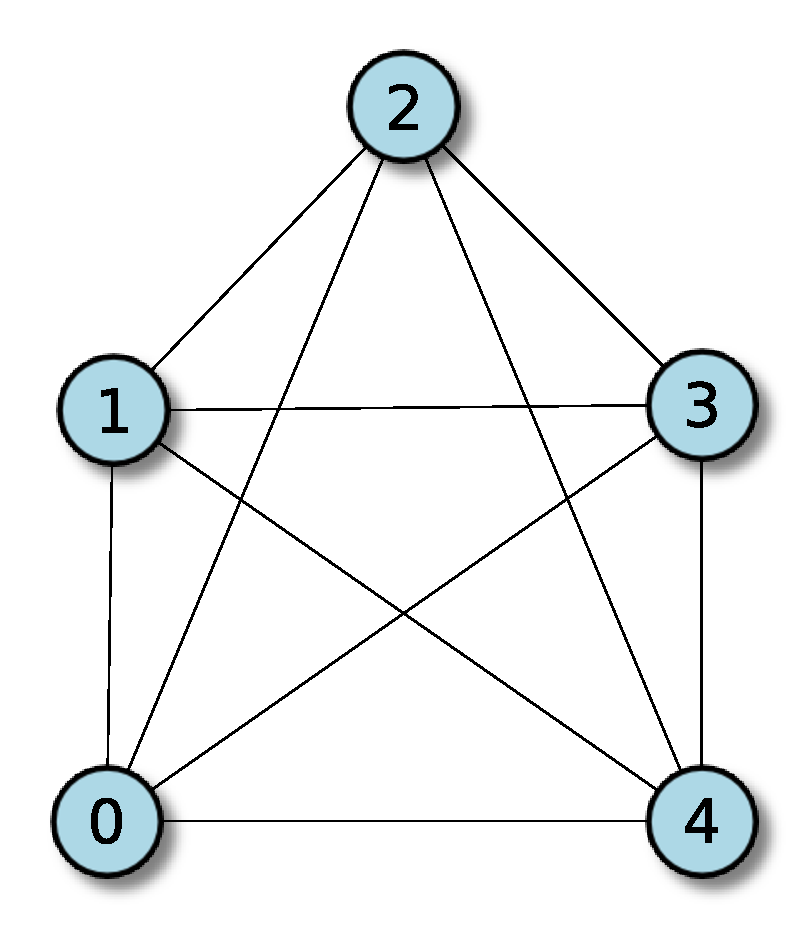
\includegraphics[height=.21\textheight]{pics/K5plain} & 
  \hspace{.10\textwidth} &
  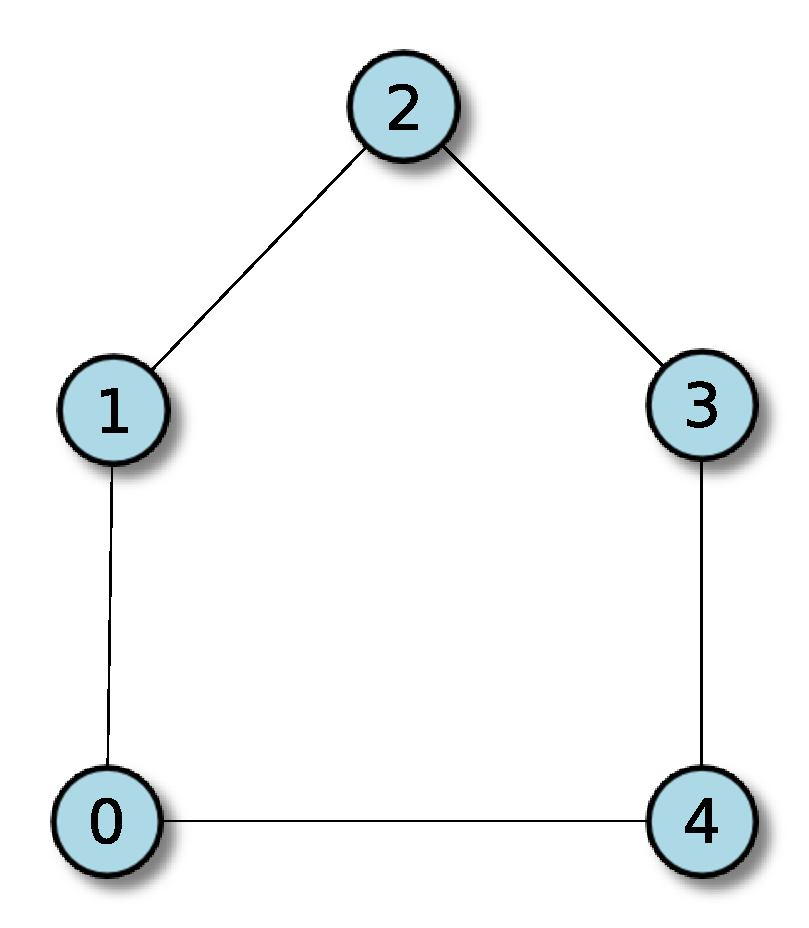
\includegraphics[height=.21\textheight]{pics/C5}
\end{array}
$
\caption{Examples of graphs with different expansion properties.\label{fig:isoexample}}
\end{minipage}
\end{figure}

\noindent
The edges which connect a subset of vertices to its complement we will call its {\em boundary}, which is defined as follows.  
\begin{definition}
The {\bf edge boundary} of $S \subseteq V$ is the set $\partial S \subseteq E$ defined to be: 
\[  \partial S = \left\{ \left(u,v\right) \ \vert \ u \in S \ {\rm and }\  v \in V - S     \right\}  \]
\label{def:edge_boundary}
\end{definition}

There are both edge and vertex oriented definitions of expansion. We will be using {\em edge expansion} as the basis for our discussion. The {\em edge expansion } is measured by the {\em isoperimetric measure} and the {\em isoperimetric constant}.

\begin{definition}
\label{def:isoperimetric_measure}
Let $G$ be a graph and $S \subseteq V(G)$. The {\bf isoperimetric measure}  of $S$, denoted $i(G,S)$ is
\[ 
i(G,S) = \frac{\left|\partial S\right| }{ \min\left\{ \left|S \right|, \left|V - S\right|   \right\} }
\]
\end{definition}

\begin{definition}
\label{def:isoperimetric_constant} 
  Let $G$ be a graph. The {\bf isoperimetric constant} of $G$, denoted $i(G)$ is
\[
i(G) = \inf_{ \stackrel{S \subseteq V}{0 <  \left| S \right| < \infty   } } i(G,S)
\] or equivalently if $\left|V \right| < \infty $ 
\[
i(G) = \min_{\stackrel{ S \subseteq V  }{|S| \leq \frac{|V|}{2}}    } i(G,S) 
\]
\end{definition}

To gain a conceptual notion of what exactly the isoperimetric constant attempts to measure, let us compute  $i(G)$ for three graphs that lie on the extreme of connectedness. First we will show that the isoperimetric constant of a disconnected graph is zero, as any good measure of connectedness should be. 

\begin{example}[Disconnected Graph] 
 \label{ex:disconnected}
Let $G$ be any disconnected graph on $n$ vertices. We would like to show that $i\left(G\right) = 0$. To demonstrate this let $S$ be a connected component of $G$ and without loss of generality assume that $|S| \leq \frac{n}{2}$. Since $S$ is a connected component of the graph $G$ we may conclude that $\partial S =  \emptyset$. Thus   \[  0 \leq  i(G) \leq \frac{ \left|\partial S \right|}{ \left| S \right| } = 0    \]  with implies that $i(G) = 0$.
\end{example}

\noindent
Next we will compute the isoperimetric constant for a graph with minimal connectivity, the {\em cycle graph}. 

\begin{example}[Cycle Graph]
\label{ex:cycle_graph}
Let $C_n$ be the cycle graph on $n$ vertices. Let $S$ be any chain of vertices of $C_n$ of length $m$, where $m < \frac{n}{2}$. We then have that $ i\left(S,G\right) = \frac{2}{m}$. It can be shown, as in Davidoff {et~al.}~\cite{Davidoff:2003qf}, that the chain of length $m$ where $m = \lfloor \frac{n}{2} \rfloor$ does indeed minimize this ratio. Thus we can conclude that the isoperimetric constant of the cycle $C_n$ is $\frac{2}{ \left\lfloor \frac{n}{2} \right\rfloor}$. 
\end{example}


Note that as the number of vertices grows the isoperimetric constant tends toward zero. An important characteristic of {\em expanding families of graphs} is that this doesn't occur. To see a graph with the opposite asymptotic behavior we will show what the isoperimetric constant is for a graph with maximal connectivity, the {\em complete graph}.


\begin{example}[Complete Graph]
\label{ex:complete_graph}
Let $K_n$ be the complete graph on $n$ vertices.  Let $S$ be any subset of vertices with $|S| = m$ and $m \leq \frac{n}{2}$.  Since $K_n$ is the complete graph we have that $|\partial S| = m \left( n - m \right)$, which implies that \[  \frac{|\partial S|} {|S|} =  \frac{m \left( n - m \right)}{m}   = n - m  \]  Which is minimized when $m = \left\lfloor \frac{n}{2} \right\rfloor$. Thus we can conclude that the isoperimetric constant of $K_n$ is $ n - \left\lfloor \frac{n}{2} \right\rfloor = \left\lceil \frac{n}{2} \right\rceil$. 
\end{example}


The notion of an {\em expander} graph is often used to describe a graph with a relatively small number of edges and a large isoperimetric constant. While the term is used to describe an individual graph, it is defined precisely as an asymptotic quality of a family of graphs. A family of graphs whose members all meet a certain isoperimetric requirement will be know as an {\em expanding family} of graphs.

\begin{definition}
  \label{def:expanding_family}
Let $\mathcal{F} = \left\{ G_k \ \vert \ k \in \mathbb{N} \right\}$ be a collection of graphs with $| V(G_k)| = n_k$  and $n_k \rightarrow \infty$ as $k \rightarrow \infty$. Then we say that $\mathcal{F}$ is an {\bf expanding family } of graphs if there exists an $\epsilon > 0 $ such that $ \epsilon \leq i\left( G_k \right)$ for all $G_k \in \mathcal{F}$. Each $G_k \in \mathcal{F}$ is known as an {\bf $\epsilon$-expander graph} or sometimes just an {\bf expander}. 
\end{definition}


It should be noted that, as defined, the family of complete graphs $\left\{ K_n \ \vert \  n \in \mathbb{N}\right\}$ is an expanding family. Yet the family of cycle graphs $\left\{ C_n \ \vert \ n \in \mathbb{N} \right\}$ is not. Both of these families are examples that lie on the extreme ends of expansion.

The next theorem of this section will establish the connection between the notion of edge expansion and the spectrum of a regular undirected graph. This theorem was first proven independently by  Dodziuk~\cite{MR743744} and Alon-Milman~\cite{Alon:1985ys} and Alon~\cite{Alon:1986fr}. Before we state the theorem we should recall a few facts about the spectrum. The {\em spectrum} of a graph $G$ on $n$ vertices is the sequence of eigenvalues, including multiplicities, of it's adjacency matrix $A$. If $G$ is undirected then we have that $A$ is both a real and symmetric matrix, which implies that each eigenvalue $\lambda_i$ is real. Thus eigenvalues can then be listed in descending order, $\lambda_1, \lambda_2,\ldots, \lambda_n$ by which we will refer to them.  Moreover, we have that if $G$ is a $d$-regular graph then $\lambda_1 = d$ and $\left\vert \lambda_i \right\vert \leq d$ for $1 \leq i \leq n$. All of these facts, including the following theorem,  appear with proof in Davidoff {et al.}~\cite{Davidoff:2003qf}. 

\begin{theorem}
 Let $G$ be a $d$-regular graph on $n$ vertices. Then \[ \frac{d - \lambda_2  }{ 2} \leq  i(G)  \leq \sqrt{2d \left(d - \lambda_2 \right) }    \] 
\label{thm:spectral_expansion}
\end{theorem}

\noindent
The value $d - \lambda_2$ is commonly known as the {\em spectral gap} of a regular graph and this theorem is stating that there is a relationship between the combinatorial notion of {\em expansion} and the spectrum of a graph, which is an algebraic property.

Another interpretation of expansion can be expressed by analyzing a certain {\em random walk} on the graph. A random walk on a graph is a discrete-time stochastic process where each vertex can be thought of as a state in which the process occupies at a certain time. As our discrete time transitions from one step to the next the process will transition from one vertex to another with a certain probability, which we call its {\em transition probability}. The random walk which we will consider is the walk in which it is equally likely that we transition from the vertex at a given time-step to any adjacent vertex at the next time-step and there is a $0$ probability of transitioning to a non-adjacent vertex. These transition probabilities are commonly expressed using a {\em transition matrix} which, in this case of a $d$ regular graph, takes the form of the {\em normalized adjacency} matrix $\hat{A} = \frac{1}{d} A$.  It should be noted that by scaling the adjacency by a constant factor we also scale the spectrum by the same factor. Namely $\hat{\lambda}_i = \frac{1}{d} \lambda_i$ for all $1\leq i \leq n$. So in terms of this process,  an expander graph will be a graph on which this walk converges to its steady state distribution very quickly. This convergence is commonly measured by the second largest eigenvalue $\hat{\lambda}_2$ The two methods of analysis are analogous as $\hat{\lambda}_2 = \frac{1}{d} \lambda_2$ and we present it only because it is used frequently in the literature and in the next portion of our discussion.  
 
The final theorem of this section establishes the connection between the zig-zag product, denoted $G \zigzag H$ and the expansion of the constituent graphs and is due to Reingold {et al.}~\cite{Reingold:2002ys}. For simplicity's sake, we will reserve defining the zig-zag product explicitly until Definition~\ref{def:zig_zag:old} in Chapter~\ref{chapt:old_zz}. Note that by $\hat{\lambda}_i$ we are speaking of the spectrum of the random walk on the graph. 

\begin{theorem}{(The Zig-Zag Theorem, {Reingold-Vadhan-Widgerson}~\cite{Reingold:2002ys})}
\label{thm:zigzag}
\noindent
Let $G$ be a $m$-regular graph on $n$ vertices and let $H$ be a $d$-regular graph on $m$ vertices and let $\alpha, \beta$ be such that \[ \hat{\lambda}_2(G) \leq \alpha \quad \hat{\lambda}_2(H) \leq \beta  \]  Then $G \zigzag H$ is a $d^2$ regular graph on $nm$ vertices where the function $\hat{\lambda}_{2}(G \zigzag H)$ satisfies the following:
\begin{itemize}
\item If $\alpha < 1$  and $\beta < 1$ then $\hat{\lambda}_{2}(G \zigzag H) < 1$.
\item  $\hat{\lambda}_{2}(G \zigzag H) \leq \alpha + \beta$.
\item $\hat{\lambda}_{2}(G \zigzag H) \leq 1 - \frac{\left(1 - \beta^{2} \right)\left(1-\alpha \right)}{2}$.
\end{itemize}
\end{theorem}
\noindent
Since the bound of the normalized eigenvalue $\hat{\lambda}_{2}\left(G \zigzag H\right)$ depends only on the eigenvalues of $G$ and $H$ the first bound does indeed imply that if $G$ and $H$ both have good expansion then $G \zigzag H$ does also. This is due to the fact that when the normalized spectrum is bounded away from one the spectral gap is non vanishing, which implies that the isoperimetric measure is also bounded away from zero as discussed earlier.  

The product described in Theorem~\ref{thm:zigzag} have been used in Reingold {et al.}~\cite{Reingold:2002ys} to iteratively construct a family of graphs of constant vertex degree with bounded expansion parameter. The proof that this family of constant degree graphs uses the bounds stated in item 2 and 3 in Theorem~\ref{thm:zigzag}. For details of this construction see also Hoory {et al.}~\cite{Hoory:2006bh}.

What has been omitted to this point is that when we speak of {\em the} zig-zag product of $G$ and $H$ we, and much of the literature, have left out an important detail, the fact that with two fixed constituent graphs there are really many zig-zag products, some of which are non-isomorphic. The focus of this thesis will be to explore the differences among these products. We begin by defining the zig-zag, and related, {\em replacement} products on regular graphs, much like the original authors, but with a few changes which will highlight the ways in which replacement products may differ. Then we will develop a complete characterization of the different classes of zig-zag and replacement products of a small, but non-trivial, special case. And finally we will conclude the thesis with a generalization of the zig-zag product that will be called the {\em sandwich product}, which will allow for many of the restrictions (such as regularity on the constituent graphs) to be removed.  


\chapter{The Replacement and Zig-Zag Products}
\label{chapt:old_zz}

In this chapter we will define the {\em zig-zag} and {\em replacement} graph products in the manner similar to that outlined by Hoory {et al.\ }\cite{Hoory:2006bh} with only a few changes in notation. For the duration of this chapter we assume: 

\begin{itemize}
\item $G$ is a $m$-regular graph on $n$ vertices.
\item $H$ is a $d$-regular graph on $m$ vertices, $\left\{0,\ldots,m-1\right\}$.
\item $G$ and $H$ are both undirected and have no loops and no multi-edges.  
\item For each $u \in \vertS{G}$, $N_{u}$ is the set of vertices which are adjacent to $u$.  
\end{itemize}

\noindent
Since $G$ is a $m$ regular graph and $H$ has $m$ vertices we can, for each $u \in \vertS{G}$, define a bijection $\enum_{u}: N_{u} \to \vertS{H}$. We will call this bijection the {\em local-enumeration} of $u$ with respect to $H$ and the collection  \[ \Enum_{G} = \left\{ \enum_{u} \ \vert \ u \in \vertS{G}  \right\}   \] the {\em enumeration} of $G$ with respect to $H$. One can think of these enumerations as just an edge labeling which allows for us to establish a direct correspondence between the edges of $G$ with the vertices of $H$.

\section{The Replacement Product}
\label{sec:replacement-product}

Once we have established an enumeration of $G$ with respect to $H$, we can define the following graph product
:
\begin{definition}
\label{def:replacement_product}
The {\bf replacement} product of $G$ with $H$ and enumeration $\Enum$, denoted $G \replacement_{\Enum} H$, is the graph with vertex set $\vertS{G} \times \vertS{H}$ for which $\left( u, a \right)$ is adjacent to $ \left( v, b \right)$ if either
\begin{enumerate}
\item \label{itm:rep_zig} $u = v$ and $\left( a, b\right) \in E(H)$, or
\item  \label{itm:rep_zag} $u \neq v$ and  $\left( u, v \right) \in \edgeS{G}$ where $\enum_{u}\left( v \right) = a $ and $\enum_{v}\left(u\right) = b$.
\end{enumerate}
\end{definition}

The replacement product can be thought of as the union of two graphs on the same set of vertices. The first is a disjoint union of $n$ copies of $H$, one for each vertex of $G$ (as described by item~\ref{itm:rep_zig} in Definition~\ref{def:replacement_product} ).  We will follow the terminology of Reingold {et al.}~\cite{Reingold:2002ys} and Hoory {et al.}~\cite{Hoory:2006bh} in calling these copies of $H$, ``clouds'' or a $u$-cloud when designating the particular vertex is important.  The second graph is a collection of edges between clouds which is given to us by the enumeration of $G$ that we had fixed earlier (item~\ref{itm:rep_zag} in Definition~\ref{def:replacement_product}).  We will call these edges the ``bridges'', or ``bridge edges'',  of $G \replacement H$. It should be noted that the clouds described in item~\ref{itm:rep_zig} of Definition~\ref{def:replacement_product} are constructed independent of the enumeration of $G$. 

Different enumerations of $G$ yield different replacement products, this can be seen in  Figure~\ref{fig:replacement} which depicts two non-isomorphic graphs resulting from the replacement product of $K_5$ and a 4-cycle, $C_{4}$ that has been generated by different enumerations. There are $\left(m!\right)^n$ different possible enumerations of $G$ with respect to $H$, some will yield isomorphic graphs and some will not.

\begin{figure}[h!]
\centering
\begin{minipage}{.80\textwidth}
$
\begin{array}[h]{ccc}
  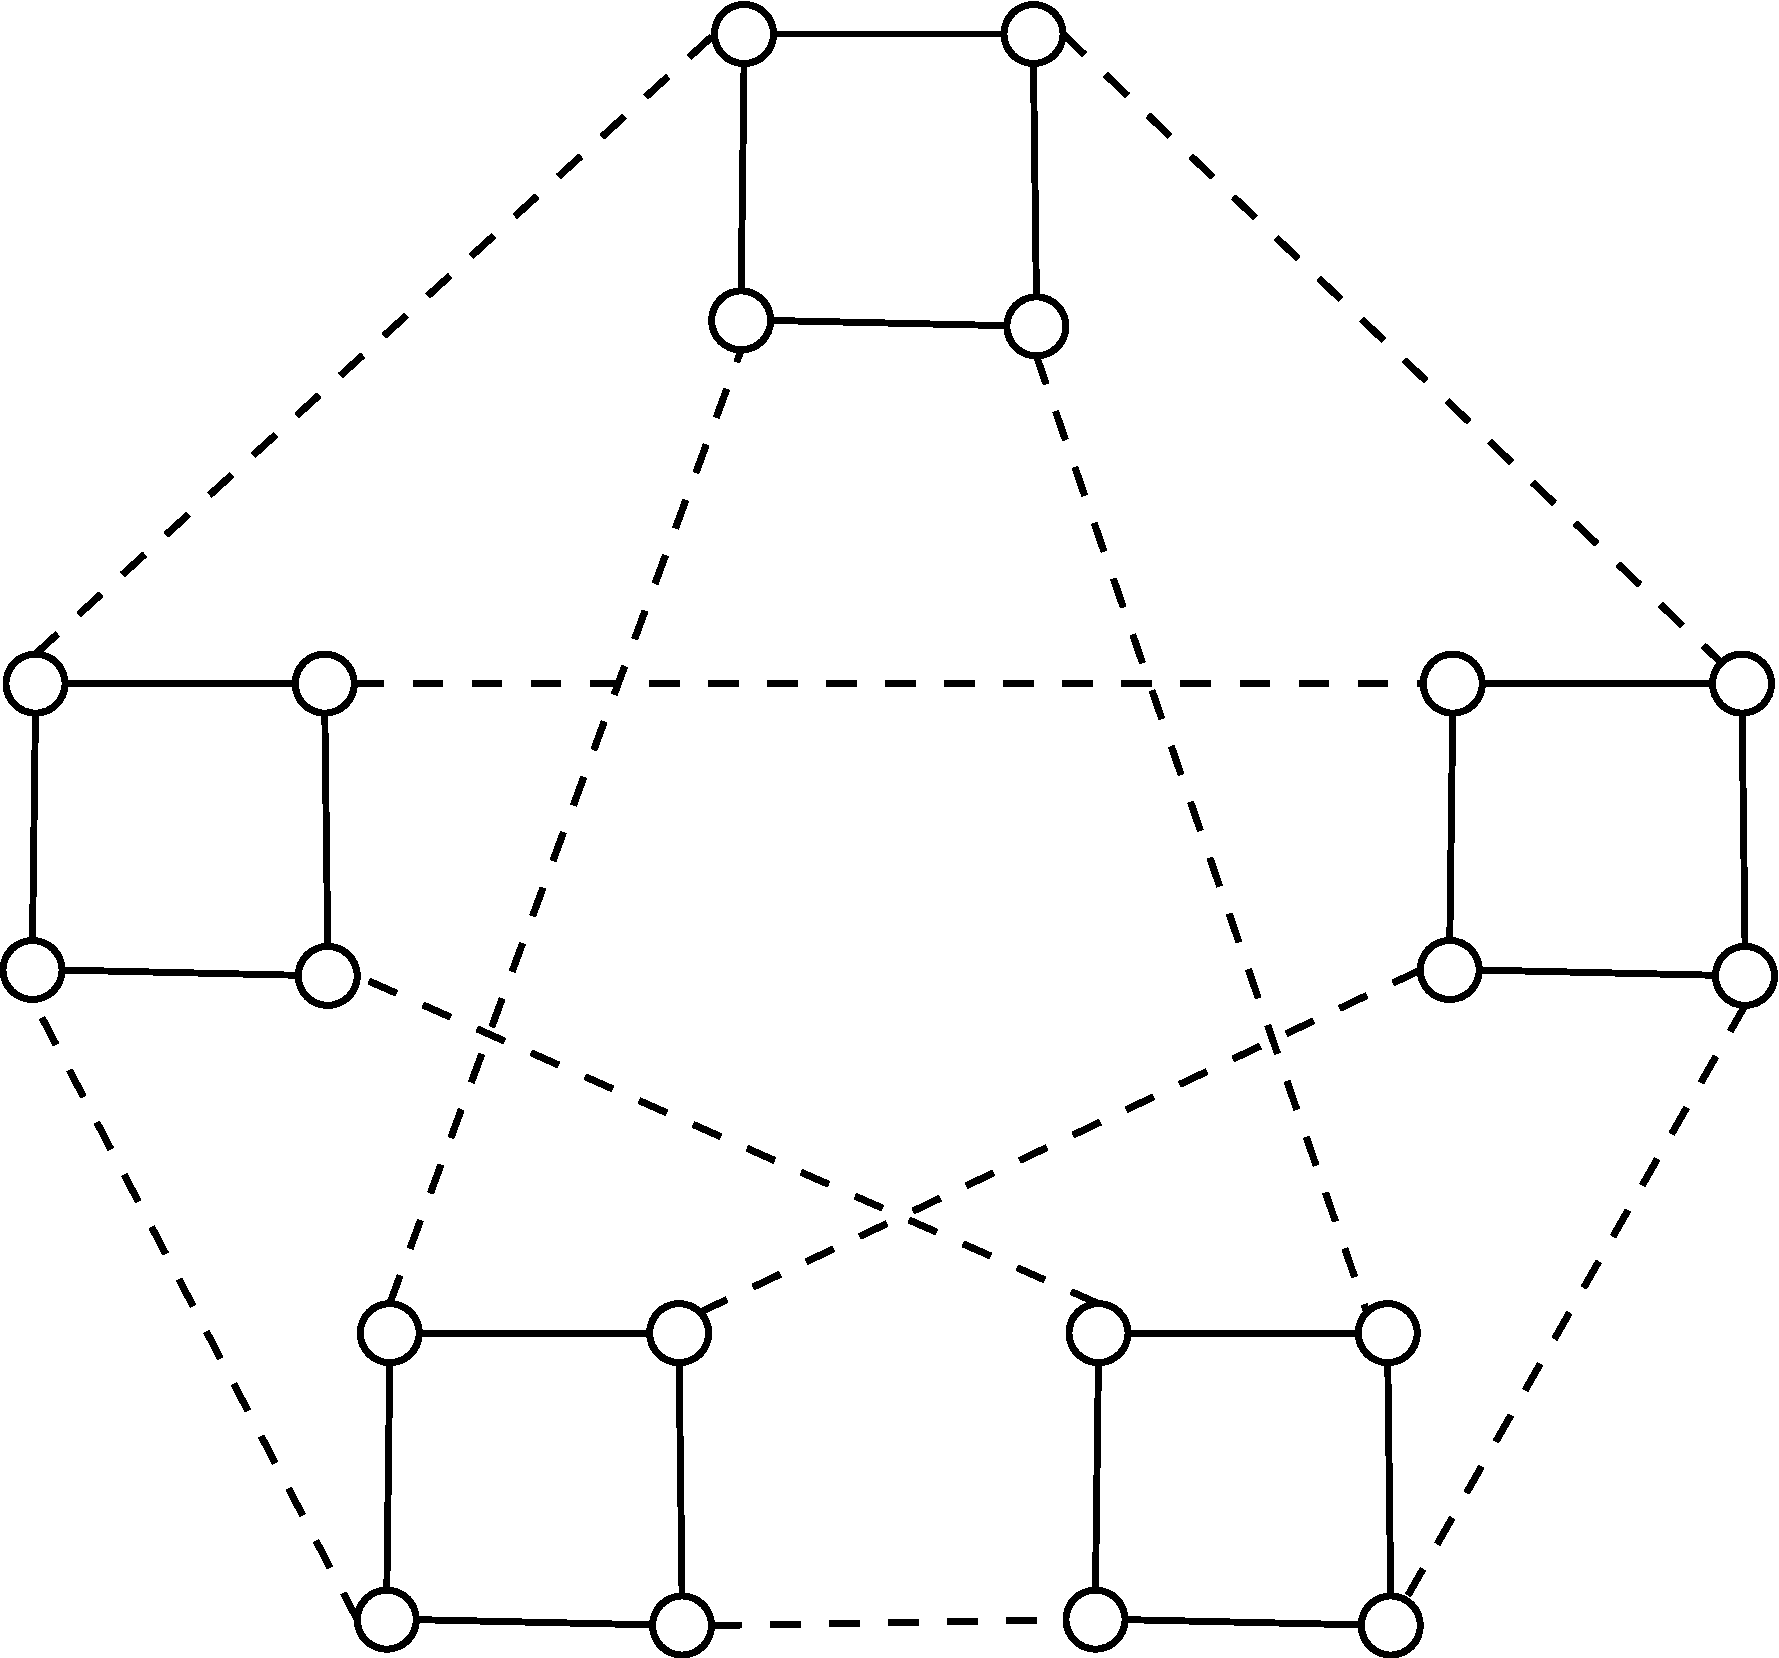
\includegraphics[width=.4\textwidth]{pics/replacementK5_C4} &
  \hspace{.13\textwidth} &
  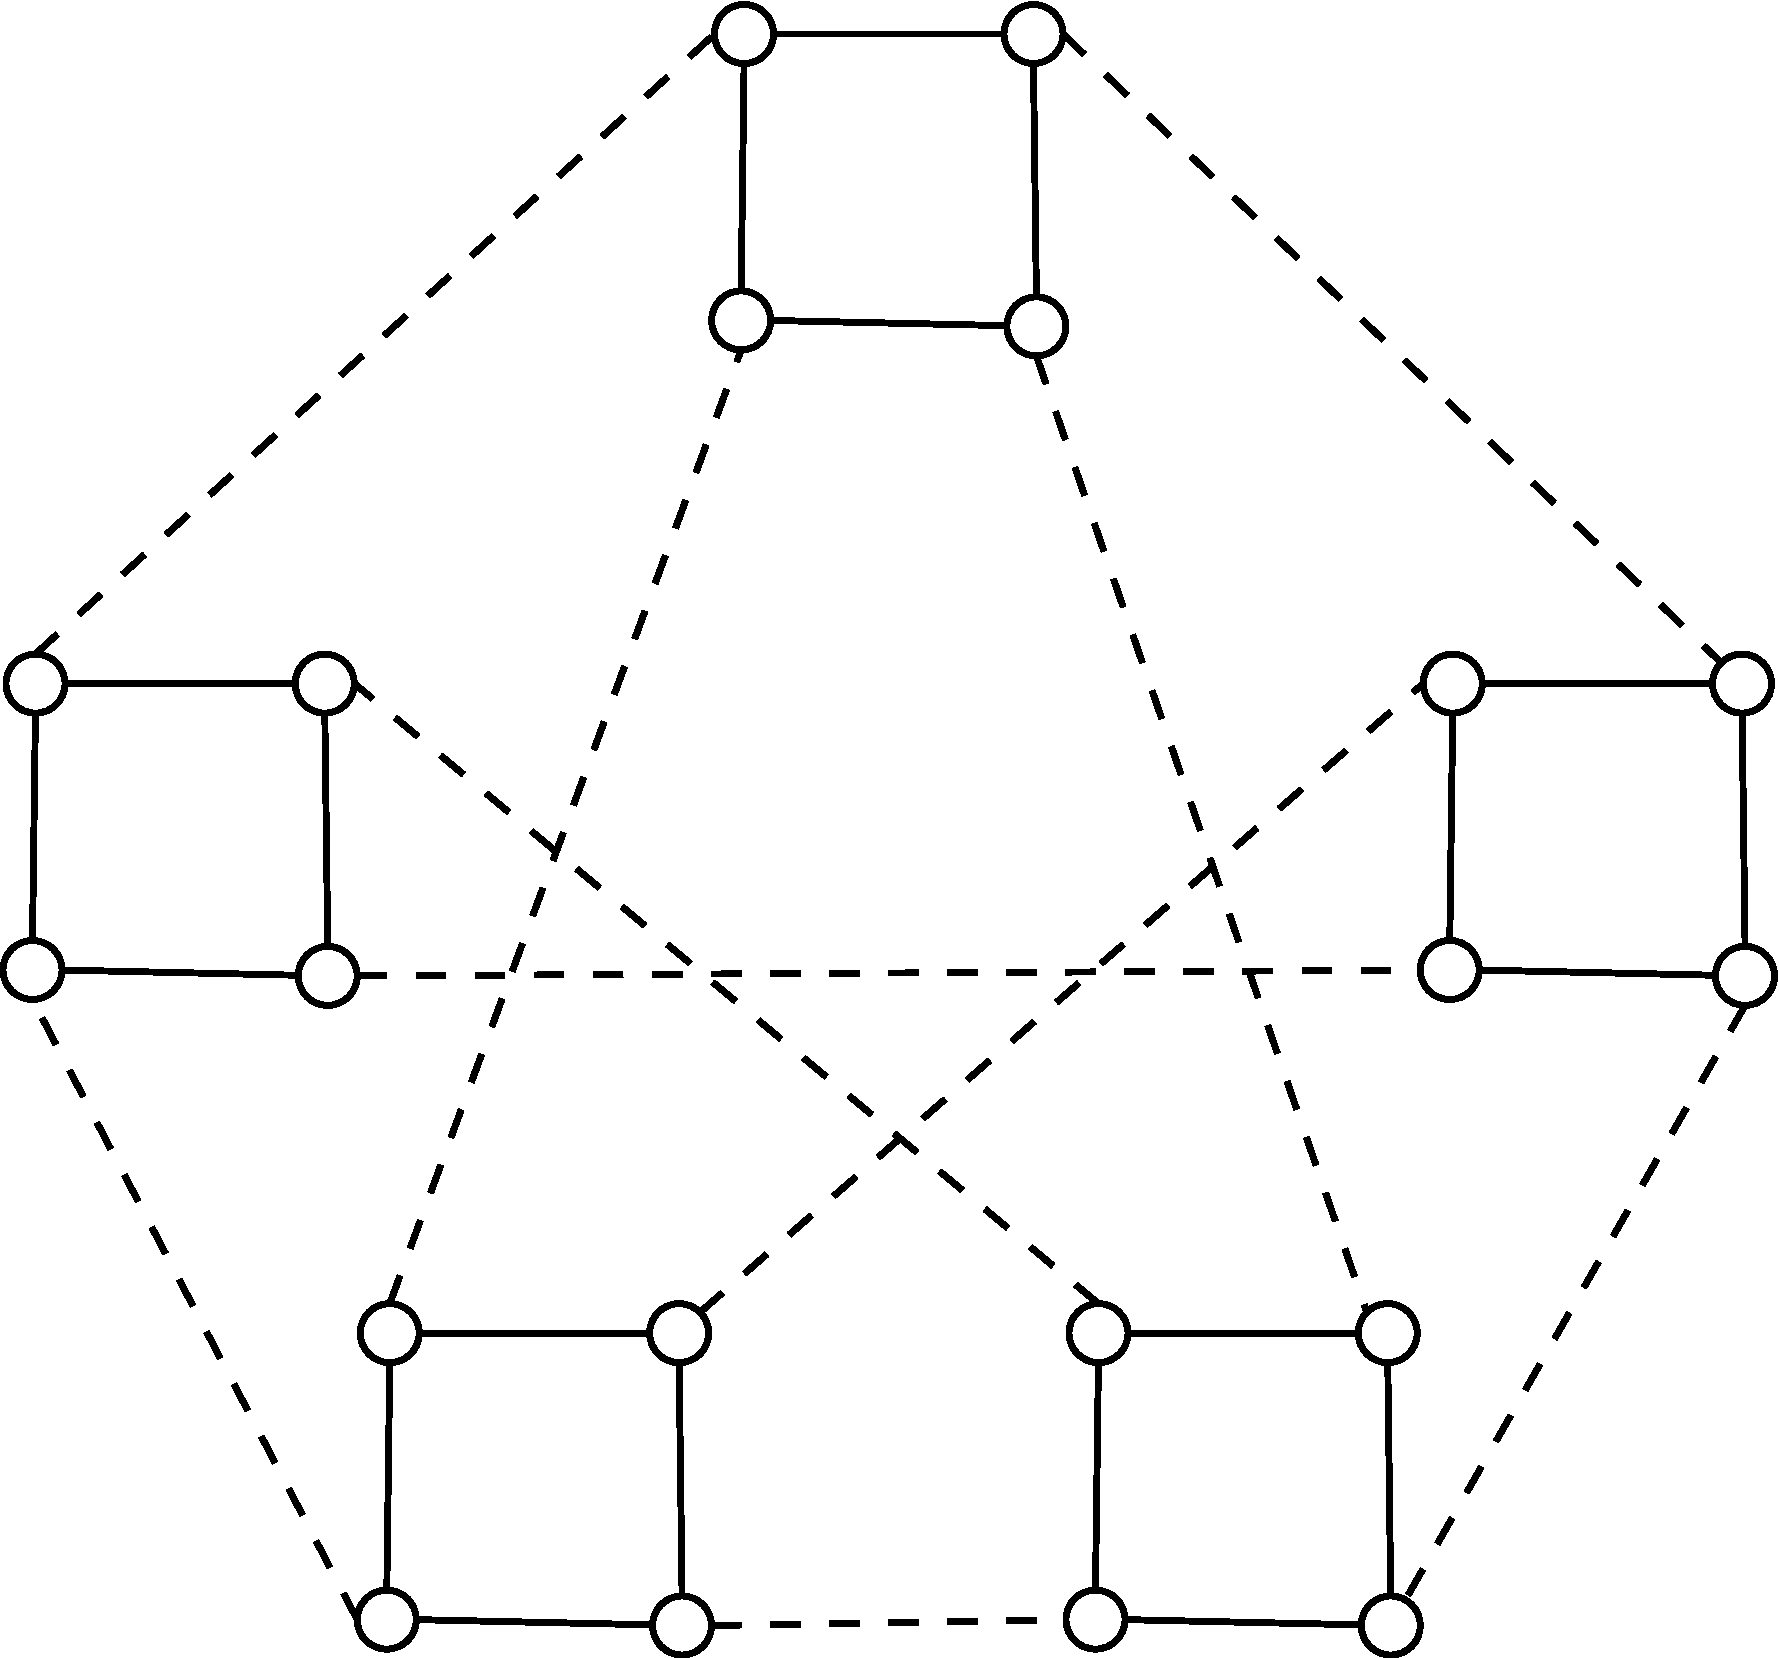
\includegraphics[width=.4\textwidth]{pics/replacementK5_C4_2}
\end{array}
$
\caption{Both graphs are Replacement Products of $K_5$ with a 4-cycle, but using different enumerations of the edges of $K_5$.  The first graph may be seen to be bipartite, while the second has cycles of odd length, so the two are not isomorphic.\label{fig:replacement}}
\end{minipage}
\end{figure}

We will next define what we mean by a {\em replacement product} isomorphism, which is a one-to-one correspondence between both the verticies and the enumerations which will preserve the structure of the graphs. This function has a very specific form that will be outlined in the following proposition:
 
\begin{proposition}
\label{prop:replacement_prod_iso}
Let $\Enum$ and $\Enum^{\prime}$ be two enumerations and let $G \replacement H$ and $G \replacement^{\prime} H$ be the associated replacement products.  Let $f \in \Aut(G)$ and, for each $u \in \vertS{G}$, let $g_u \in \Aut(H)$. Define the function $F$ mapping $\vertS{G}\times \vertS{H}$ to itself, by $F(u,a) = (f(u), g_u(a))$. $F$ is an isomorphism  from $G \replacement H$ to $G \replacement^{\prime} H$ if  $\enum^{'}_{f(u)}( f(v)) = g_u(\eta_u ( v))$
\end{proposition}
\begin{proof}

Suppose that $\enum^{'}_{f(u)}( f(v)) = g_u(\eta_u ( v))$ for each $u, v$. For the proof we just have to check that $F$ preserves adjacency. Let $(u,a)$ and $(u,b)$ be adjacent in $G \replacement H$. Then since $g_u \in \Aut(H)$, it follows directly that $(f(u), g_u(a))$ is adjacent to $(f(u), g_u(b))$ in $G \replacement^{\prime} H$.

Now consider adjacent vertices $(u,a)$ and $(v,b)$ for $u \neq v$.  We must show that $(f(u), g_u(a))$ is adjacent to $(f(v), g_v(b))$. By definition, $(u,v) \in \edgeS{G}$, $(f(u),f(v)) \in \edgeS{G}$ and $\enum_{u}(v) = a $ and $\enum_{v}(u) = b$. The result follows directly from our supposition. 

\noindent
Note we could also have written the statement is equivalent to
\[\enum^{\prime}_u(v) = g_u(\enum_{f^{-1}(u)} (f^{-1}(v) ))\  \textrm{for all}\  u,v \]
and to
\[ \enum_u(v) = g_u^{-1}(\enum^{\prime}_{f(u)}(f(v))) \]
\end{proof}


\begin{definition}
  \label{def:replacement_isomorphism}
We call a function $F$ that satisfies the properties of Proposition~\ref{prop:replacement_prod_iso} an {\bf replacement product isomorphism}, or sometimes just an rp-isomorphism.
\end{definition}

\noindent 
Definition~\ref{def:replacement_isomorphism} says, that a replacement product isomorphisms preserves 

\begin{itemize}
\item The structure of each independent cloud,
\item The bridges between each cloud as provided by the adjancencies of $G$ and it's enumeration.
\end{itemize}

\noindent
Whether or not this completely characterizes every isomorphism that preserves the replacement structure is still an open question; however preliminary results point strongly toward this conclusion.

% \begin{lemma}
% \label{lemm:equivrelation}
% Let $G \replacement H \simeq G \replacement^{\prime} H$ if they are isomorphic as replacement products. Then $\simeq$ is an equivalence relation.    
% \end{lemma}
% \begin{proof}
% Since $F \in \Aut(G \replacement H)$ by proposition~\ref{prop:replacement_prod_iso}. All relevant properties (reflexivity, symmetry and transitivity) are all inherited from the its membership in $\Aut(G \replacement H)$
% \end{proof}

\begin{theorem}
\label{thm:upperbound_iso}
Let $n( G \replacement H)$ be the number of unique non-isomorphic replacement products. Then we have \[ n(G \replacement H) \leq \left(\frac{m!}{\left| \Aut(H)\right|}  \right)^{n}  \]
\end{theorem}
\begin{proof}
Let $f \in \Aut(G)$ be the identity automorphism and consider $g = \left( g_{u_1}, g_{u_2}, \ldots, g_{u_n} \right)$ for $g_{u_k} \in \Aut(H)$. Then for each $G \replacement H$ with fixed enumeration $\Enum$ we have that $G \replacement H \simeq F(G \replacement H)$. This implies that the equivalence class of replacement products that are isomorphic to $G \replacement H$ has at least $\left| \Aut(H) \right|^n$ members. Thus since we have that there are at most $(m!)^{n}$ total enumerations we can conclude that there are at most $ (m!)^{n} / \left| \Aut(H) \right|^{n}$ different equivalence classes. This establishes the desired result.
\end{proof}
It follows from this theorem that for all $3$-regular graphs the replacement product taken with the cycle graph on $3$ vertices is unique, up to a graph isomorphism.

\begin{example}
  Let $G$ be any $3$-regular graph on $n$-vertices and consider the cycle graph on three vertices $C_3$. Thus since we have that $\Aut(H) = D_3$, Theorem~\ref{thm:upperbound_iso} implies that \[  n(G \replacement C_3 ) \leq \left( \frac{ 3! }{ \card{D_3}} \right)^n = \left( \frac{6}{6} \right) = 1    \] which implies that there is only one replacement product of $G$ with $H$ up to isomorphism.
\end{example}

\section{The Zig-Zag Product}
\label{sec:zig-zag-product}

With the replacement product in mind, we  discuss the {\em zig-zag} product.  The vertex set is $V(G) \times V(H)$, and the edges connect the endpoints of certain walks of length three of a ``zig-zag'' nature in $G \replacement H$. By a ``zig-zag'' walk, we mean a walk that traverses

\begin{enumerate}
\item An edge within one {\em cloud} (zig).
\item An edge connecting one {\em cloud} to another (zag).
\item An edge within the final {\em cloud} (zig again).
\end{enumerate} 
\noindent
Figure~\ref{fig:zigzag} illustrates this procedure for one vertex in the replacement product

\begin{figure}[h!]
\centering
\begin{minipage}{.42\textwidth}
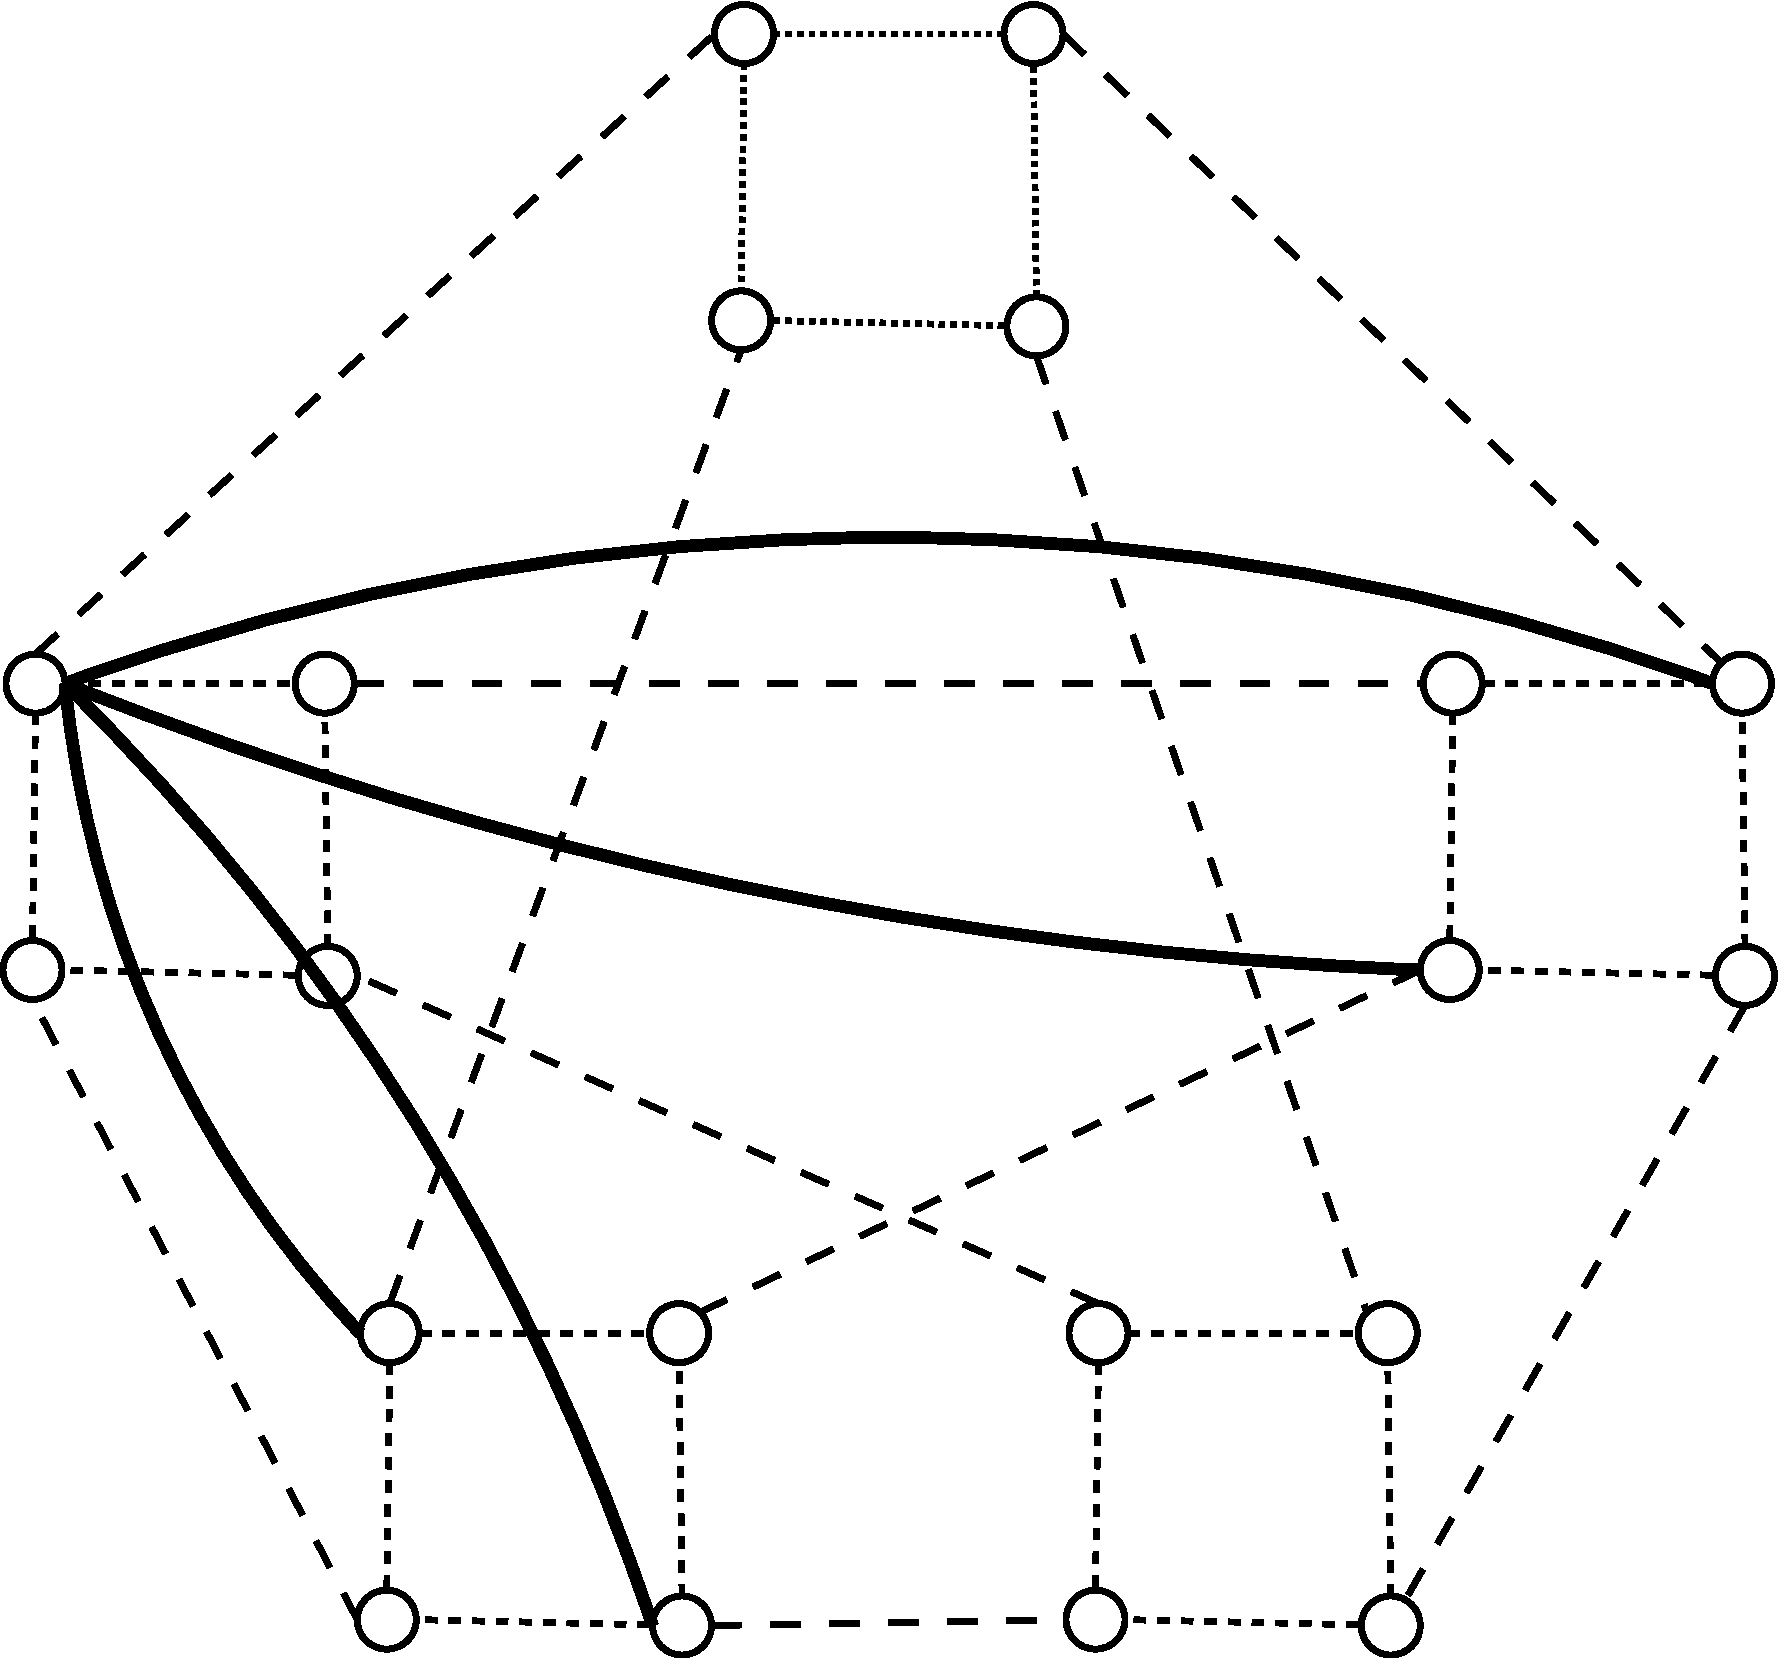
\includegraphics[height=.28\textheight]{pics/zig_zagK5_C4}
\caption{The four ``Zig-Zag'' edges incident to a single vertex in a Replacement Product of $K_5$ with a 4-cycle. \label{fig:zigzag}}
\end{minipage}
\end{figure}
\noindent

\begin{definition}
\label{def:zig_zag:old}
The {\bf zig-zag} product of $G$ with $H$ (for a given enumeration $\Enum$), denoted $G \zigzag H$, is a graph with vertex set $V(G) \times V(H)$ for which $\left( u, a \right)$ is adjacent to $ \left( v, b \right)$ if and only if $\left(u,v\right) \in \edgeS{G}$ and both $\left(a, \enum_{u}(v) \right)$ and $\left(\enum_{v}(u), b\right)$ are in $\edgeS{H}$.
\end{definition}


\begin{theorem}
\label{def:isomorphic_replacement:zigzag}
Let $\Enum$ and $\Enum^{\prime}$ be enumerations of $G$ with respect to $H$ such that an isomorphism of replacement products, $F: G \replacement H \to G \replacement^{\prime} H$ exists (as in Definition~\ref{def:replacement_isomorphism}). Then $G \zigzag H$ is isomorphic to $G \zigzag^{\prime} H$ and $F$ is that isomorphism. 
\end{theorem}
\begin{proof}

Consider $F$ as a bijection of $\vertS{G} \times \vertS{H}$ into itself. We would like to show that $F$ is an edge preserving mapping of $G \zigzag H$ onto $G \zigzag^{\prime} H$. Let $\left(u, a \right), \left(v, b \right) \in \vertS{G \zigzag H }$ be such that $\left(u, a \right)$ and $\left(v, b \right) $ are adjacent in $G \zigzag H$. This implies that both
\begin{enumerate}
\item $\left(u,v\right) \in \edgeS{G}$, and
\item $\left(a, \enum_{u}\left( v\right)\right), \left(\enum_{v}\left(u\right), b\right) \in \edgeS{H}$.
\end{enumerate}
Since $F(u,a) = \left( f(u), g_{u}(a) \right)$ and $F(v,b) = \left( f(v), g_{v}(b) \right)$. We have that
\begin{enumerate}
\item $\left( f(u), f(g) \right) \in \edgeS{G}$ since $f \in \Aut(G)$,
\item $\left(g_u(a), g_u(\enum_{u}(v)) \right)$ and $\left(g_v(\enum_{v}(u)), g_v(b) \right)$ and in $\edgeS{H}$, and
\item  $\enum^{\prime}_{f(u)}(f(v)) = g_u( \enum_u(v) )$ and $\enum^{\prime}_{f(v)} (f(u)) = g_u( \enum_v(u)) = g_u(\enum_{v}(u))$.
\end{enumerate}
The converse implication follows similarly.
\end{proof}

The literature pertaining to the zig-zag product has a tendency to fix a certain, though usually unspecified, enumeration of $K_5$ and speak of the product graph in the singular. In the process of writing this thesis we noticed that there were interesting differences between products, things like disconnected components, using different enumerations. To investigate this further, in the next section we will completely characterize the zig-zag product on the smallest example for which different enumerations can yield non-isomorphic products, $K_5$ and $C_4$. 

\chapter{The Complete Classification of $K_5 \protect \replacement C_4$ and $K_5 \protect \zigzag C_4$}
\label{chapt:K5zzC4}

\begin{quote}
The art of doing mathematics consists in finding that special case which contains all the germs of generality.

\hfill {\bf -David Hilbert}

\end{quote}

The zig-zag and replacement products are defined both by their constituent graphs and an association between them which we have named an enumeration. In this chapter we will present an analysis of these products of $K_5$ with $C_4$ as we iterate through all $ \left(4! \right)^5 = 7962624$ possible enumerations. We will show that the resultant product graphs can be categorized, up to replacement product isomorphism, into $5$ classes for the zig-zag product and $7$ for the replacement product. The hope is that by outlining this procedure, many of the techniques used will be useful to the analysis of the zig-zag and replacement products in greater generality. 

$K_5$ and $C_4$ were chosen for this exercise both for their simple geometry and the fact that their zig-zag product is the smallest example, in terms of vertices and edges, which can be either connected or disconnected. Since one of the principal applications of the zig-zag product is to aid in the construction of families of expander graphs, expansion being a measure of connectivity, we felt that the disconnected zig-zag product was of particular interest.

Throughout this chapter, let $\vertS{K_5} = \left\{0,1,2,3,4 \right\}$ and $\vertS{C_4} = \left\{0,1,2,3 \right\}$, with adjacency defined in the most natural manner \[ \edgeS{K_5} = \left\{(i,j)\ \vert \ i,j \in [5]\ i \neq j \right\} \quad \textrm{and} \quad \edgeS{C_4} = \left\{ (i,j) \ \vert \ i = j \pm 1 \bmod 4 \right\} \]

\section{Enumerations and Parity Cycle Decompositions}
\label{sec:enum-parity-cycle}

We will begin by first considering two concrete enumerations of $K_5$. For each of these enumerations we will construct a sequence of disjoint (in terms of edges) closed walks on $K_5$. Each of these closed walks will have an analogous structure in $K_5 \replacement C_4$ and $K_5 \zigzag C_4$ that will be unique, up to order and orientation,  with respect to the enumeration of $K_5$ chosen. In this section the results will be given without proof, and are meant only to introduce the reader to the intuition and to provide some context for further analysis. The two enumerations presented will correspond to two major classes of the $K_5 \zigzag C_4$; one which is connected while the other has more than one connected component.

Figure~\ref{fig:10-example} shows the first enumeration of  $K_5$ that will be considered, along with the associated zig-zag and replacement product.  On this graph consider the {\em closed walk} on $K_5$, \[ \ppath = \left[  0\ 1\ 2\ 3\ 4\ 2\ 0\ 3\ 1\ 4 \right].   \]  The closed walk $\ppath$ has a length $10$ and reaches each vertex of $K_5$ exactly two times while traversing each edge of $K_5$ once. If the closed walk uses no duplicate edges then we will call it  a {\em circuit}. Though our notation lists only vertices it is implied that it includes each edge defined by consecutive vertices, and also the edge from $4$ to $0$ that closes the walk. The circuit $\ppath$ also has the property that the edge traversed while approaching a vertex along the walk has the same {\em parity}, with respect to the local enumeration of that vertex,  as the edge traversed when leaving. For example in $\ppath$ we approach the vertex $1$ through the edge $(0,1)$ and leave through $(1,2)$ which have local enumeration $0$ and $2$ with respect to the vertex $1$. Following the path as listed, we later approach $1$ though the edge $(3,1)$ and leave through $(1,4)$ which has an enumeration of $1$ and $3$ respectively. Each pair of edges has the same parity, and if we require that our walk traverses each edge exactly once, we can conclude, up to starting vertex and order in which we list the vertices, that this closed walk is unique given this enumeration.  
   
% A circuit is parity preserving if, loosely stated, a path in $K_5$ by which the path ``enters'' and ``leaves'' a particular vertex by edges that have the same local parity. For example, in Figure~\ref{fig:parity_example} we have colored the local edges in $K_5$ to correspond to their parity.  Note that the particular coloring chosen is not particularly important, just that the local coloring groups the corresponding vertices local parity properly.

\begin{figure}[h!]
  \centering
  \begin{minipage}{.85\textwidth}
  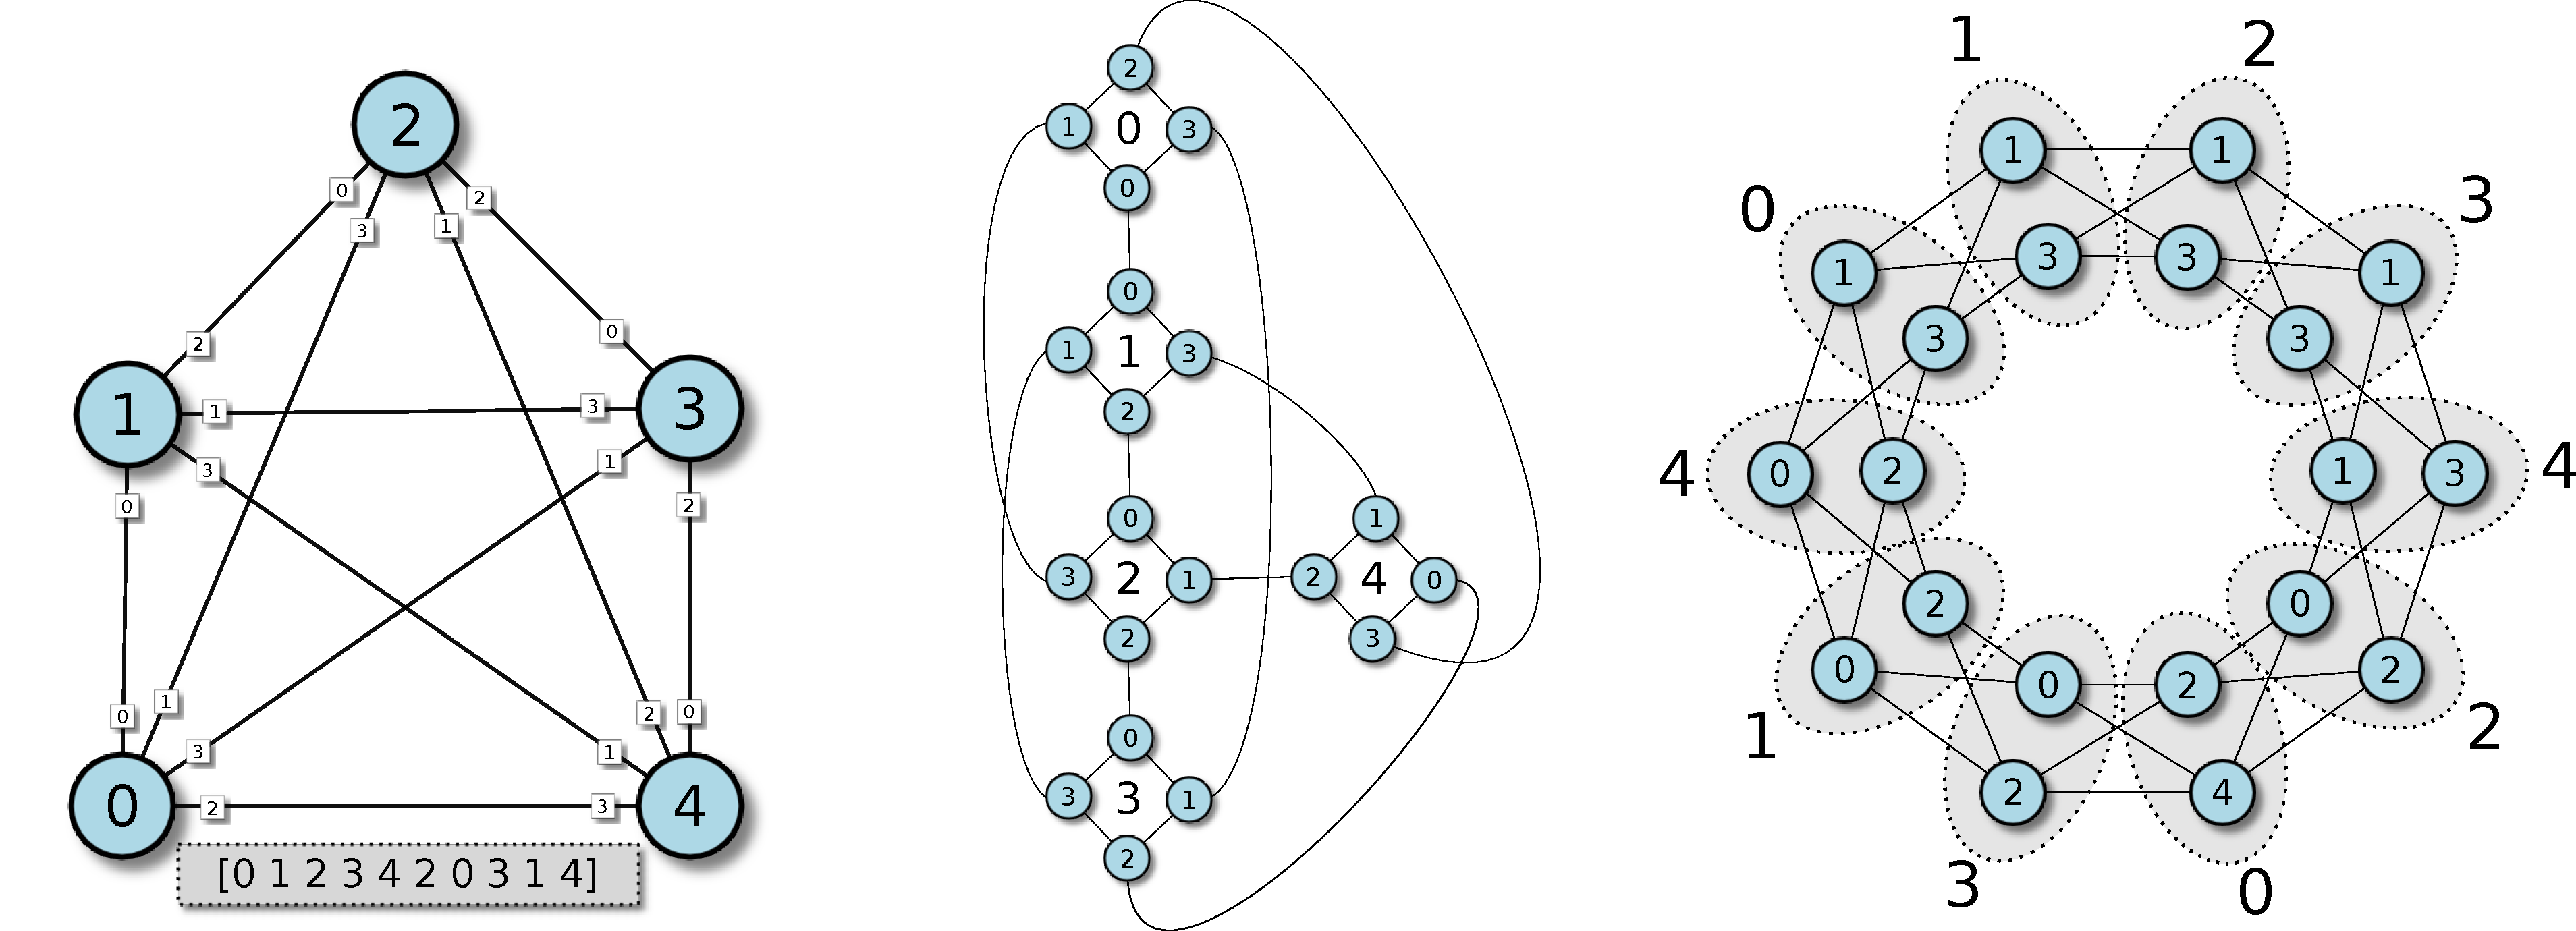
\includegraphics[width=\textwidth]{pics/10-example}
  \caption{Enumeration of $K_5$ with the corresponding Replacement and Zig-Zag Products.\label{fig:10-example}}
  \end{minipage}
\end{figure}

% \begin{figure}[h!]
% \centering
% \begin{minipage}{.75\textwidth}
%   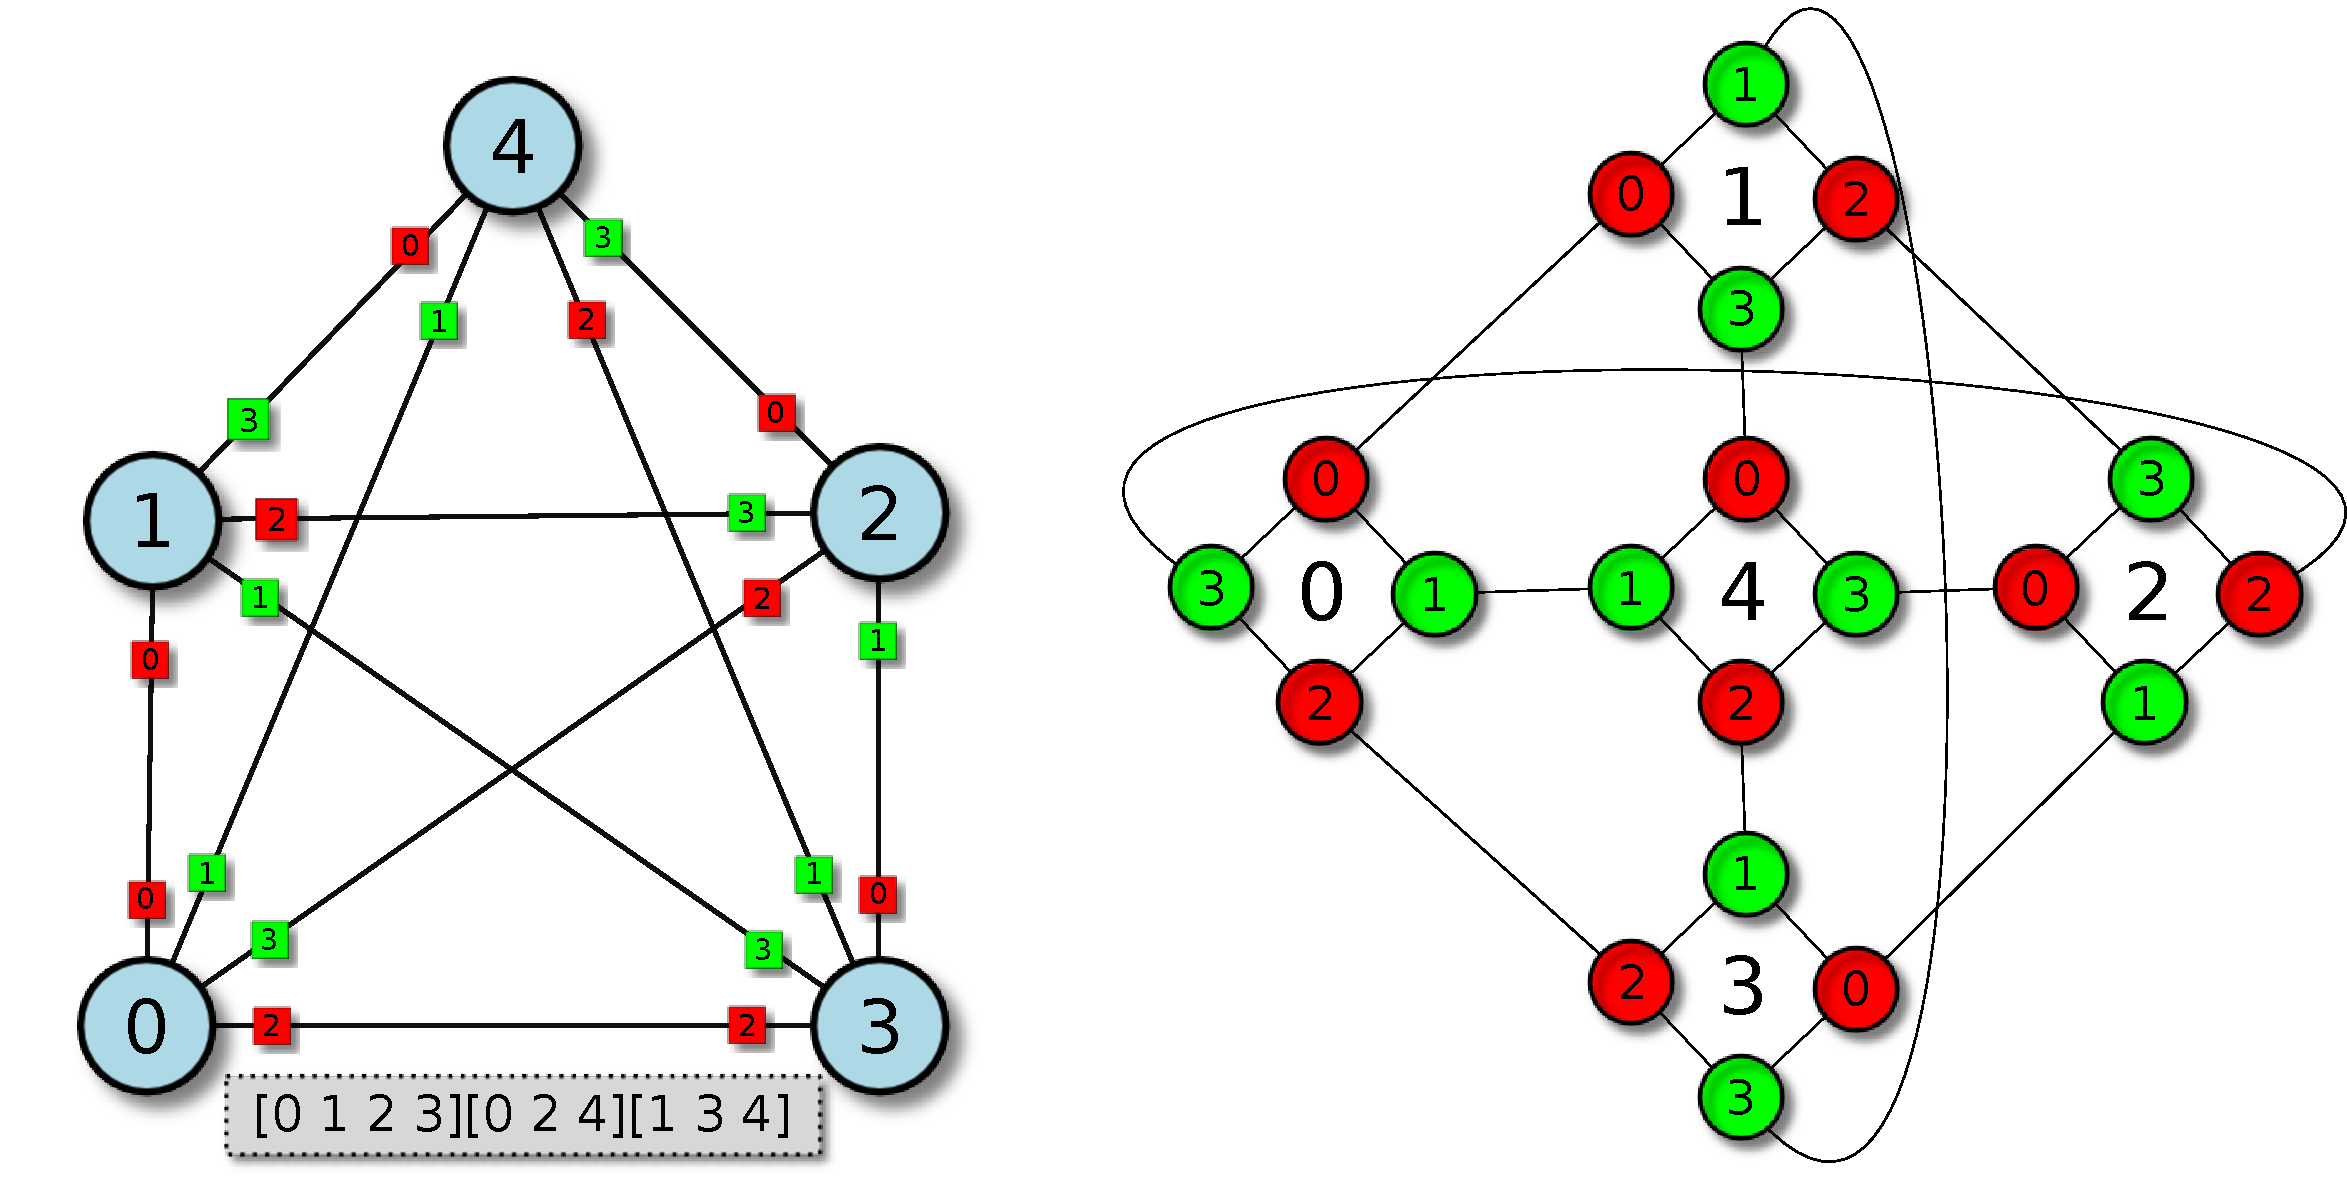
\includegraphics[width=\textwidth]{pics/parity_example}
%   \caption{$K_5$ and $K_5 \protect \replacement C_4$ colored by parity.\label{fig:parity_example}}
% \end{minipage}
% \end{figure}

The reader at this moment may question the relevance of these closed walks to the zig-zag and replacement product. Their utility lies in the fact that these {\em parity-preserving } closed walks in $K_5$\footnote{These parity preserving walks serve the same correspondence in any $4$-regular graph when the products are taken with the cycle graph on 4 vertices.} correspond exactly to analogous structures both in the replacement and zig-zag products. In the replacement product the correspondence can be constructed simply by replacing each appearance of the term ``vertex'' with ``vertex cloud''. While in the zig-zag product each stop on our walk can be associated with a pair of vertices which constitute a {\em slice} of a {\em $2$-trellis} graph. One can follow these associations by following the paths depicted in Figure~\ref{fig:10-example}.

The second enumeration of $K_5$ that will be considered is depicted, with replacement and zig-zag product, in Figure~\ref{fig:37-example}.

\begin{figure}[h!]
  \centering
  \begin{minipage}{.80\textwidth}
   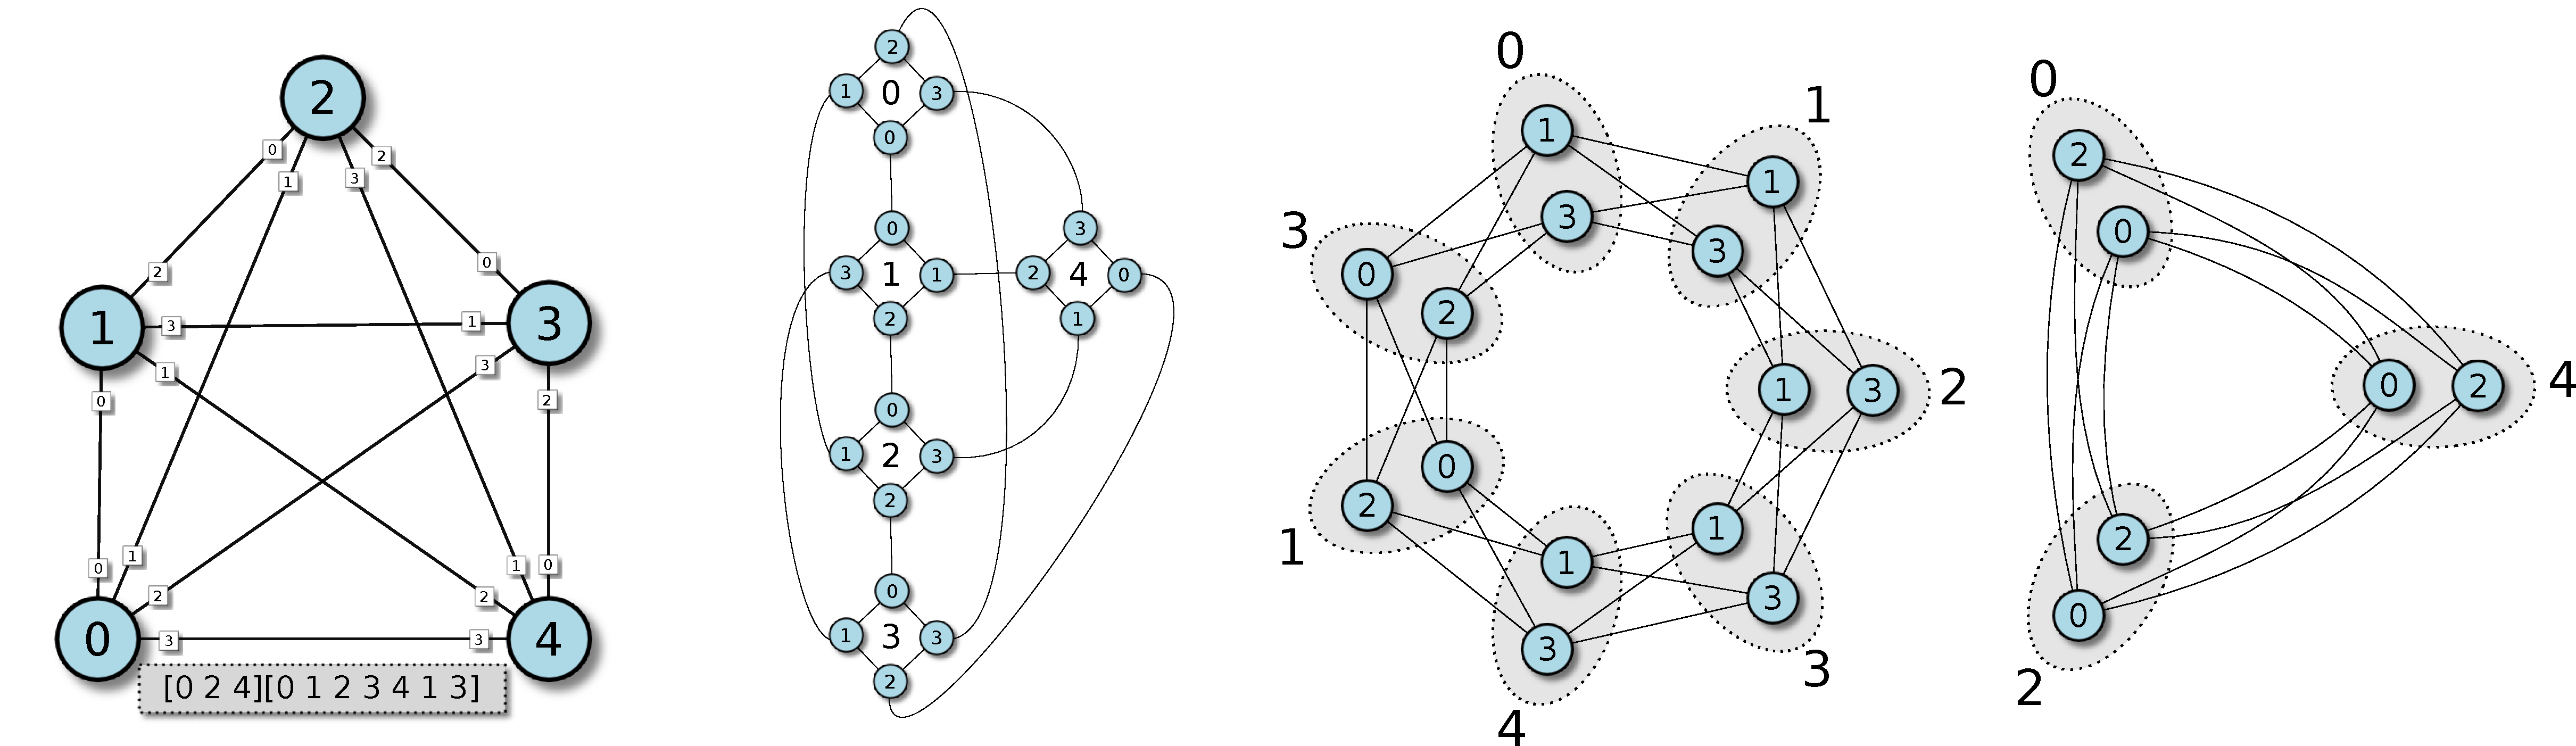
\includegraphics[width=\textwidth]{pics/37-example}
  \caption{$K_5$ with enumeration, $K_5 \protect \replacement C_4$, and $K_5 \protect \zigzag C_4$.\label{fig:37-example}}
  \end{minipage}
\end{figure}

For this particular enumeration, consider the closed walk of length $7$, $\ppath_1 = \left[0\ 1\ 2\ 3\ 4\ 1\ 3 \right]$. This closed walk satisfies the same parity requirements described above, but there are edges of $K_5$ that we haven't traversed.  Because of this we will take a closer look at the complement, in terms of edges, of this walk which is illustrated in Figure~\ref{fig:7cycle_comp}.   

\begin{figure}[h!]
  \centering
  \begin{minipage}{.50\textwidth}
  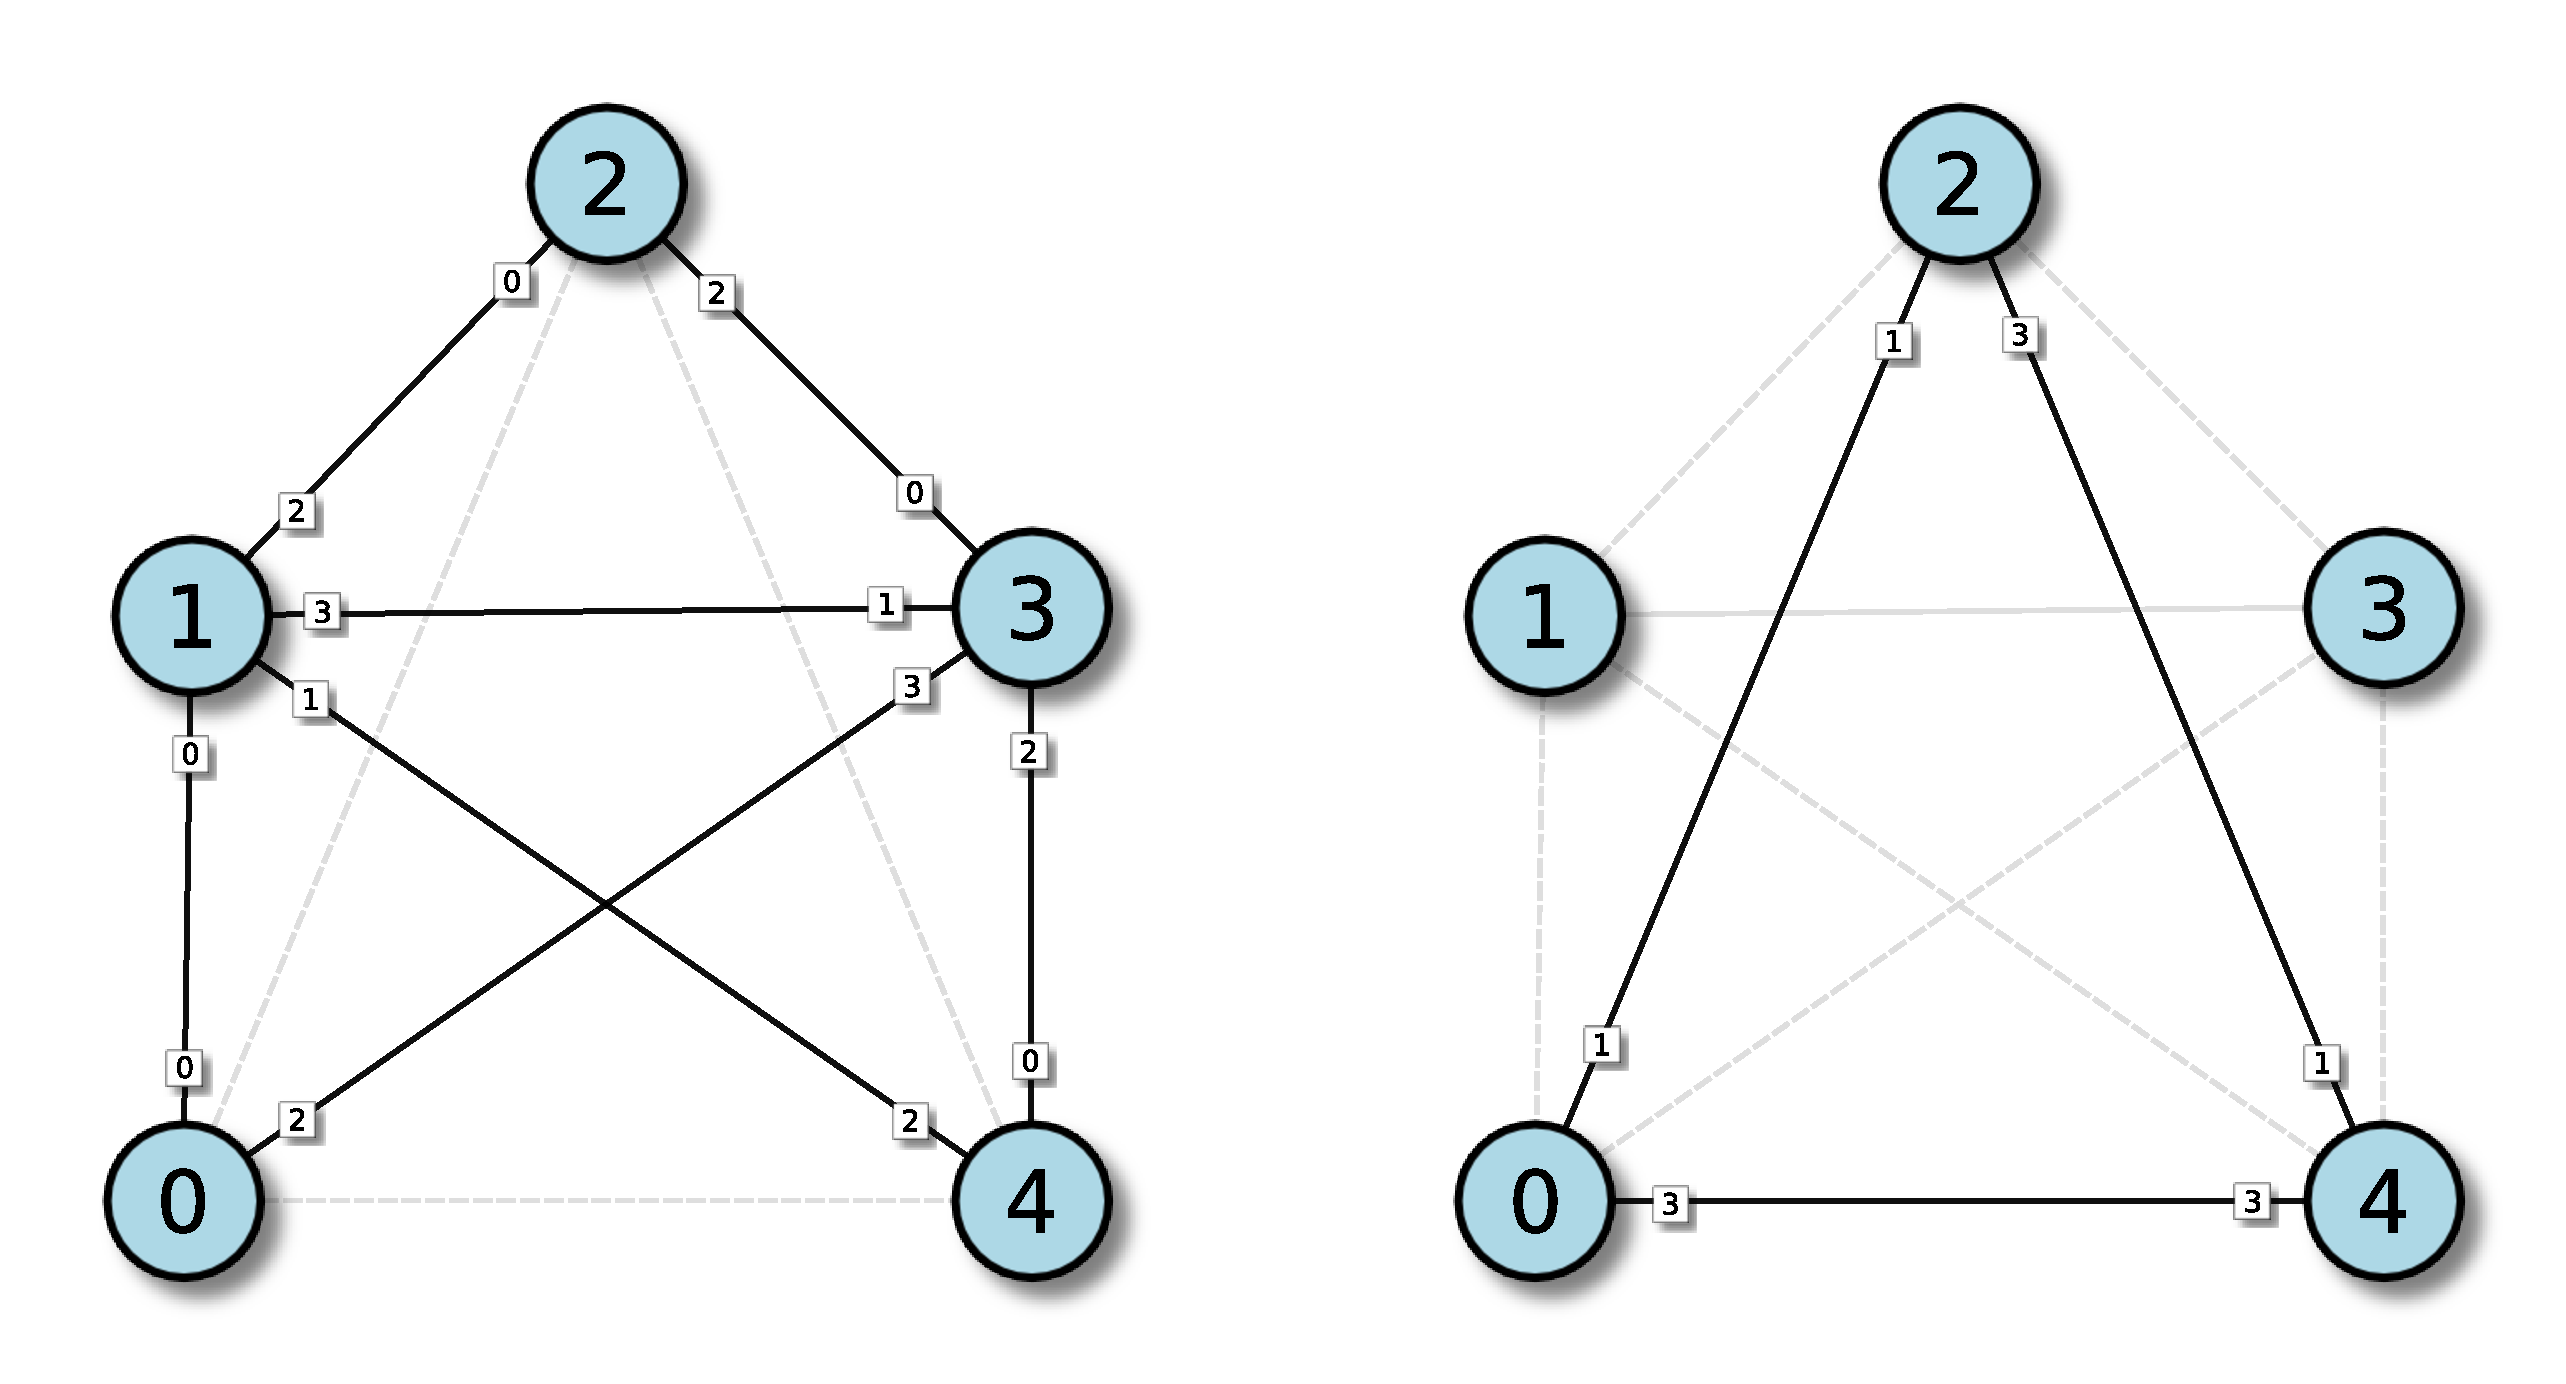
\includegraphics[height=.20\textheight]{pics/7cycle-K5-37-example} 
  \caption{Parity circuit of length 7 and its complement in $K_5$.\label{fig:7cycle_comp}}
  \end{minipage}
\end{figure}

All of the edges in $K_5 \setminus \ppath$ incident to the same vertex have the same parity. This will mean that we can construct a closed walk of length $3$, $\ppath_2 = \left[0\ 2\ 4 \right]$, contained completely within the complement. Moreover when considered together $\left[ 0\ 1\ 2\ 3\ 4\ 1\ 3 \right]$ and $\left[0\ 2\ 4 \right]$ exhaust all of the edges of $K_5$ and satisfy the same parity requirements. We will call the collection of disjoint closed walks that satisfy the parity requirements and exhaust the edges of $K_5$ the {\em parity circuit decomposition} of $K_5$ with respect to a given enumeration. This collection is completely determined by the enumeration given. This fact will be demonstrated in subsequent sections.

% As in the prior example each of these closed walks corresponds to features of $K_5 \replacement C_4$ and $K_5 \zigzag C_4$. For each parity circuit there is a corresponding circuit structure contained in the replacement and the zig-zag products, which is illustrated in Figure~\ref{fig:37-example}. Within the replacement product, we will call the circuit a {\em bridge circuit} and in the replacement product and in the zig-zag product a {\em $2$-trellis circuit}. It should be noted that each parity circuit in $K_5$ corresponds to a component in the zig-zag product and that each component has a very similar structure.


\section{The Parity Circuit Decompositions of $K_5$}
\label{sec:count-parity-circ}

With the correspondence between parity circuits and the structure of $K_5 \replacement C_4$ and $K_5 \zigzag C_4$ hinted at earlier but not rigorously developed we will devote this section to establishing theorems reveling the structure of parity circuit decompositions. Throughout this section all of the enumerations are of $K_5$ with respect to $C_4$. We are now ready to define the {\em parity circuit}, which will be of particular importance to our analysis. 

\begin{definition}
  \label{def:pcircuit}
Let $\ppath = \left[ u_1\  u_2\  \cdots\  u_k \right]$ be a closed walk on $K_5$ with enumeration $\Enum$. Then we say that $\ppath$ is a {\bf parity circuit} of length $k$ if both 
  \begin{itemize}
  \item For each $u_{i} \in \ppath$,  $\enum_{u_i}( u_{i-1}) = \enum_{u_{i}}(u_{i+1}) \pm 2 \bmod{4}$ where $i$ is computed modulo $k$. 
  \item No edge is traversed more than once. 
  \end{itemize} 
\end{definition}

It should be noted that when we discuss a particular parity circuit $\ppath$, we are really discussing the equivalence class of parity circuits modulo cyclic shifts and the order in which the vertices are listed. For example the parity circuits  $\left[ 0\ 1\ 2\ 3\ 4\ 1\ 3 \right]$ and  $\left[4\ 3\  2\  1\  0\  3\  1 \right]$ are equivalent because the same set of edges is traversed whereas $\left[0\ 1\ 4\ 2  \right]$ and $\left[1\ 0\ 4\ 2 \right]$ are not since $1$ and $2$ are neighbors of $4$ in one and not the other.
\noindent
With that established we proceed to the existence of such a structure, given a fixed enumeration of $K_5$, a starting vertex $u_0$ and an initial edge $\left(u_0, u_1\right)$.

\begin{theorem}
  \label{thm:p-circuit_existance}
Consider $K_5$ with enumeration $\Enum$ and let $\left(u_0 , u_1 \right) \in \edgeS{K_5}$ be an edge.  Then there exists a unique parity circuit $\ppath$ with $\left(u_0, u_1\right)$ as it's first edge.   
\end{theorem}
\begin{proof}
  \label{pf:p-circuit_existance}

We will show that the output of Algorithm~\ref{alg:pcircuit} is indeed a parity circuit. It is clear that, for all but the terminating edge, the walk which is output by this algorithm satisfies the parity requirements. Thus we must only show that the walk $\ppath$ is closed, traverses no duplicate edges, that the terminating edge satisfies the parity requirements, and that $\ppath$ is unique.  
  
\begin{algorithm}[b]
\caption{Construct a parity circuit $\ppath$ with initial edge $\left(u_0, u_1 \right)$.}
\label{alg:pcircuit}
\begin{algorithmic}
  \REQUIRE A graph $G$ with enumeration $\Enum$ and initial edge $\left(u_0,u_1\right)$
  \ENSURE Parity circuit $\ppath = \left[ u_0\  u_1\ \ldots\  u_k  \right]$
  \STATE $i \leftarrow 1$ 
  \WHILE{$u_{i} \neq u_{0}$ \OR $\enum_{u_i}^{-1}\left( \enum_{u_{i}}\left(u_{i-1}\right) + 2 \bmod{4}\right) \neq u_{1} $}  
  \STATE Let $u_{i+1} = \enum_{u_i}^{-1}\left(\enum_{u_{i}}\left(u_{i-1} \right) + 2 \bmod{4}\right)$
  \STATE Add edge $\left(u_{i}, u_{i+1} \right)$ to walk $\ppath$ 
  \STATE $i \leftarrow i + 1$ 
  \ENDWHILE
\end{algorithmic}
\end{algorithm}

First let us show that Algorithm~\ref{alg:pcircuit} produces a walk $\ppath$ that does not traverse an edge more that once. To do so, assume that there does exist an edge that gets traversed more than once and that such an edge, in the order which the algorithm traverses edges, is the first edge traversed twice by our algorithm. This implies that there exist $k > 0$ and $i < k$ such that $\left(u_{i-1}, u_{i} \right) = \left(u_{k-1} , u_{k} \right)$ and that this occurs for no smaller $k$. Since these two edges are equal but were traversed at the $i-th$ and $k-th$ step of the algorithm this implies that 

\begin{align*}
    \enum_{u_{k-1}}\left( u_{k-2} \right) + 2 \bmod{4} &= \enum_{u_{i-1}}\left(u_{i-2} \right) + 2 \bmod{4} &       \\
    \enum_{u_{k-1}}\left( u_{k-2} \right) \bmod{4} &= \enum_{u_{i-1}}\left(u_{i-2} \right) \bmod{4} & \\
\end{align*}

\noindent
Now since $u_{i-1} = u_{k-1}$ we can conclude that  $\enum_{u_{k-1}} = \enum_{u_{i-1}}$, which by arithmetic and the fact that $\enum_{u_{k-1}}$ is invertible, leads us to conclude that $u_{k-2} = u_{i-2}$ and $\left(u_{k-2}, u_{k-1} \right) = \left(u_{i-2}, u_{k-2}\right)$. However this is a contradiction, since the edges $\left(u_{k-1}, u_{k} \right)$ was assumed to be the first such duplicate edge. Therefore the walk in $\ppath$ cannot traverse the same edge twice. 

Next we would like to show that this algorithm terminates and that the resultant walk is closed. Since the algorithm does not traverse the same edge twice and the edges of $K_5$ are finite we can conclude that the algorithm does indeed terminate. Suppose that the algorithm does terminate when $i=k$. When the terminating condition is satisfied this implies that both $u_{k} = u_{0}$ and $\enum_{u_k}^{-1}\left( \enum_{u_{k}}\left(u_{k-1}\right) + 2 \bmod{4}\right) = u_{1}$. Since $u_{k} = u_{0}$ we have that the last edge added to $\ppath$ is $\left(u_{k-1}, u_0 \right)$ which implies that the walk is closed. Since $\enum_{u_k}^{-1}\left( \enum_{u_{k}}\left(u_{k-1}\right) + 2 \bmod{4}\right) = u_{1}$, we have that $\enum_{u_{0}}\left(u_{k-1}\right) + 2 \bmod{4} = \enum_{u_0}\left(u_{1} \right)$ which implies that this terminating edge satisfies the parity requirements. Thus we can conclude the $\ppath$ is a parity circuit.

Finally we would like to show that the parity circuits are unique. Suppose that we have two parity circuits $\ppath = \left[u_0\ u_1\ \ldots\ u_{k} \right]$ and $\ppath^{\prime} = \left[ u^{\prime}_0\  u^{\prime}_1\ \ldots\  u^{\prime}_j    \right]$ both which share an edge $\left( u_0,u_1  \right)$. Without loss of generality we can assume that this is the initial edge of both $\ppath$ and $\ppath^{\prime}$, if not, then cyclically shift and re-orient the direction of both walks until it is. Since $\left(u_0, u_1 \right) = \left( u^{\prime}_0, u^{\prime}_1 \right)$ we have that $u_0 = u^{\prime}_{0}$ and $u_1 = u^{\prime}_1$. This implies that $\enum_{u_1} = \enum_{u^{\prime}_1}$ and that 
\begin{align*}
  \enum_{u_i}\left( u_0  \right) &= \enum_{u^{\prime}_{1}}\left( u^{\prime}_0 \right) \\
  \enum_{u_1}\left( u_0  \right) +2 \bmod{4} &= \enum_{u^{\prime}_{1}}\left( u^{\prime}_0 \right) + 2 \bmod{4} \\
   \enum^{-1}_{u_1} \left( \enum_{u_1}\left( u_0  \right) +2 \bmod{4} \right) &=  \enum^{-1}_{u^{\prime}_1} \left(\enum_{u^{\prime}_{1}}\left( u^{\prime}_0 \right) + 2 \bmod{4}\right)
\end{align*}

\noindent
which implies that $u_2 = u^{\prime}_2$. By proceeding inductively we can show that $\ppath$ and $\ppath^{\prime}$ are identical, thus the parity path $\ppath$ with initial edge $\left(u_0, u_1 \right)$ is unique. 
\end{proof}
\noindent
Figure~\ref{fig:sage_pcircuit} contains a listing of Sage code which implements Algorithm~\ref{alg:pcircuit}. 
\noindent 

\begin{figure}[h!] 
\begin{sageblock}
def parity_circuit(enum, init_vert, init_enum):

    inv_enum = dict([[v, inverse_dict(d)] for v,d in enum.iteritems()])
    
    
    circ = [init_vert]
    cur_vert = init_vert
    out_enum = init_enum

    next_vert = enum[cur_vert][out_enum]
    circ.append(next_vert)
    in_enum = inv_enum[next_vert][cur_vert]
    out_enum = (in_enum + 2)%4
    cur_vert = next_vert

    
    while ( (cur_vert, out_enum) != (init_vert, init_enum) ):
        next_vert = enum[cur_vert][out_enum]
        circ.append(next_vert)
        in_enum = inv_enum[next_vert][cur_vert]
        out_enum = (in_enum + 2)%4
        cur_vert = next_vert
        
    return circ
\end{sageblock}
\caption{Sage code for generating parity circuits.\label{fig:sage_pcircuit}}
\end{figure}

To count and classify the types of parity circuits, we must first establish a theorem involving the length of a parity circuit.

\begin{lemma}
  \label{lem:smallest_pcircuit}
The smallest parity circuit in $K_5$ is of length $3$. 
\end{lemma}
\begin{proof}
  \label{pf:smallest_pcircuit}

Figure~\ref{fig:37-example} is an example of an enumeration which contains a parity circuit of length 3, so we must just show that there can be no smaller parity circuits. A parity circuit cannot be of length 2 since any closed walk of length 2 would necessarily traverse the same edge twice. Furthermore we cannot allow for a closed walk of length one without allowing for loop edges. 
\end{proof}

\noindent
To be able to use the parity circuit as a tool for classification we must first show how different parity circuits, using the same enumeration, relate to each other. Namely whether or not they can be used as a method to partition the edges of $K_5$. The first such theorem having to do with {\em disjoint } parity cycles. 

\begin{definition}
  \label{def:pcd}
Consider the sequence of parity circuits $\pcd = \left( \ppath_1, \ppath_2, \ldots, \ppath_j \right)$. We call this sequence a  {\bf parity circuit decomposition (PCD)} of $K_5$ if 
\begin{itemize}
\item For each $i$, $\ppath_i$ is a parity circuit per Definition~\ref{def:pcircuit}.
\item $\ppath_i$ and $\ppath_j$ are edgewise disjoint for $i \neq j$.
\item For each $e \in \edgeS{K_5}$ there exists a parity circuit $\ppath_i$ such that $e$ is traversed by $\ppath_i$. 
\end{itemize}
\end{definition}


\begin{theorem}
 \label{thm:unique_pcd}
For a given enumeration, $\Enum$,  there exists a unique parity circuit decomposition, $\pcd_{\Enum}$. 
\end{theorem}

\begin{proof}

We can show the existence by following a simple algorithm. Select an edge $(u_0, v_0 )$ at random and construct the parity circuit $\ppath_0$ beginning with this edge using Algorithm~\ref{alg:pcircuit}. If $\ppath_0$ exhausts the edges of $K_5$ then we are done. If not let $\ppath_{1}$ be the parity circuit which begins with edge $( u_1, v_1 )$  where $(u_1, v_1 )$ isn't traversed by $\ppath_0$. $\ppath_0$ and $\ppath_1$ will be disjoint by the uniqueness of parity circuits and then if they exhaust the edges of $K_5$ then you are done. If not, then assume that we can construct a sequence of pairwise disjoint parity circuits $\ppath_0, \ppath_1, \ldots, \ppath_{k-1}$. Once again if these exhaust the edges then this is our decomposition. If not then let $\ppath_k$ to be the parity circuit which begins with edge $\left( u_k, v_k \right)$ where $\left( u_k , v_k\right)$ is not traversed by any member of the sequence $ \ppath_0, \ppath_1, \ldots, \ppath_{k-1} $. Once again $\ppath_k$ will be the disjoint from all circuits constructed for reasons discussed earlier. Since $K_5$ has a finite number of edges we are guaranteed that this inductive procedure will terminate with a sequence $\ppath_0, \ldots, \ppath_k, \ldots, \ppath_n$ of disjoint parity circuits which exhaust the edges of $K_5$ which will establish the existence of a circuit.

Uniqueness is guaranteed both by the requirement that each edge be in one parity circuit combined by the uniqueness of the parity circuit containing each edge established earlier. 
\end{proof}

\noindent
With the existence and uniqueness of parity circuit decomposition of $K_5$ with a given enumeration, we would like to define a sequence of numbers which will be used to classify each PCD, the {\em signature} of the PCD. 

\begin{definition}
  \label{def:signature}
Let $\pcd = \left( \ppath_1 , \ldots, \ppath_k \right)$ be a parity circuit decomposition of $K_5$. The list of lengths of each circuit, ordered by size, is called the {\bf signature} of the PCD. 
\end{definition}

\noindent
The following lemmas and theorems will describe what sequences of numbers can be valid signatures.

\begin{lemma}
\label{lem:vertex2times}
Let $\pcd$ be a parity circuit decomposition of $K_5$. Then each $u \in \vertS{K_5}$ is listed exactly $2$ times in the PCD. 
\end{lemma}

\begin{proof}

Each vertex has 4 incident edges, $E_u = \left\{e_0, e_1, e_2, e_3 \right\}$. The vertex appears only one time when the edges of odd parity are traversed, namely $e_1$ and $e_3$ and another time when the edges of even parity have been traversed, $e_0$ and $e_2$. Thus the vertex appears at most two times in a PCD. Since the PCD contains all such edges we have that it appears at least two times.
\end{proof}

\begin{theorem}
  \label{thm:K_5partition10}
The signature of a parity circuit decomposition $\pcd$ is a partition of $10$ with terms no smaller than $3$. Which implies that the signature of any enumeration is equal to one of the following
\begin{itemize}
 \item $3,3,7$.
 \item $3,7$.
 \item $4,6$.
 \item $5,5$.
 \item $10$.
\end{itemize}
\end{theorem}
\begin{proof}
This theorem follows directly from Lemma~\ref{lem:vertex2times} and Lemma~\ref{lem:smallest_pcircuit}.
\end{proof}

Now that we have a way to group the enumerations, namely by the signature of the PCD of the enumeration, we will now delve further into the structures that underlie their PCD's. 

\section{Counting Parity Circuit Decompositions}

In Theorem~\ref{thm:unique_pcd} we established that for each enumeration there exists a unique parity circuit decomposition. In this section we will show how many of the $(4!)^5 = 7962624$ enumerations induce different decompositions. To address this question, we will be using the natural {\em group action} of the symmetric group $S_{4}^5$ on our enumerations which, for $\sigma \in S_{4}^5$ and $\Enum$ an enumeration,  is given by \[\acts{\sigma}{\Enum} = \left\{ \sigma_{u} \circ \enum_u\ \vert\ u\in \vertS{G} \right\}.\] Recall that a group $\mathcal{G}$ {\em acts} on a set $S$ if there exists a binary function $\mathcal{G} \times S \mapsto S$,  denoted by $\left(g,s\right) \mapsto \acts{g}{s}$, which satisfies both of the following 
\begin{itemize}
\item $\acts{gh}{\left(s\right)}= \acts{g} {\left(\acts{h}{s}\right)}$ for all $g,h \in \mathcal{G}$ and $s \in S$.
\item For the identity element $e \in \mathcal{G}$, $\acts{e}{s} = s$ for all $s \in S$.  
\end{itemize}
\noindent
It is fairly easy to show that the mapping discussed above satisfies these requirements. Most of the language which will be used is standard and can be found in most Modern Algebra Texts such as Hungerford~\cite{Hungerford:1974zr}.

Let $\EnumSet$ be the set of all enumerations of $K_5$, let $\pcdSet$ be the set of all parity circuit decompositions per Definition~\ref{def:pcd}, and let $F:\EnumSet \mapsto \pcdSet $ be the natural mapping that sends an enumeration $\Enum \rightarrow \pcd_{\Enum}$. Where is the unique, up to order and orientation, PCD generated by $\Enum$ guaranteed by Theorem~\ref{thm:unique_pcd}. We are ready to state the main theorem of this section. 

\begin{theorem}
  \label{thm:pcd_count}
The number of unique parity circuit decompositions is $3^5$
\end{theorem}
 
\noindent
To establish this fact, we will set up a one-to-one correspondence between the left cosets of  $D_{4}^5$, where $D_4$ is the dihedral subgroup of $S_4$ generated by $\left( 0 1 2 3 \right)$ and $\left( 1 2 \right) \left(0 3 \right)$, and the set of parity circuits $\pcdSet$. This correspondence is due to both how $S_4$ and $D_4$ act on our local enumerations and a correspondence between those enumerations and the PCDs. We will begin by proving a quick lemma which states a property of the action which is provided by $S_{4}^5$ which will be used later in justifying our claim.      

\begin{lemma}
  \label{lem:unique_associates}
For any  $\Enum^{0},\Enum^{1} \in \EnumSet$ there exists a unique $\sigma \in S_{4}^5$ such that $\acts{\sigma}{\Enum^{0}} = \Enum^{1}$. 
\end{lemma}

\begin{proof}
  \label{pf:unique_associates}

Let $\Enum^0,\Enum^1 \in \EnumSet$ and $u \in \vertS{K_5}$. Since $\enum_{u}^{1}$ and $\enum_{u}^{2}$ are bijections from $N_{u} \mapsto \left\{ 0, 1, 2, 3 \right\}$, $\sigma_{u}$ given by
\[
 \sigma_{u} = \left(
   \begin{array}[h]{ccc}
      \enum_{u}^{1}(e_0) &\ldots & \enum_{u}^{1} (e_3) \\
      \enum_{u}^{2}(e_0) & \ldots & \enum_{u}^{2}(e_3)  
   \end{array}
\right)
\] is a permutation in $S_4$ such that $\enum_{u}^{2} = \sigma_{u} \circ \enum_{u}^{1}$. Thus for $\sigma = \left\{ \sigma_{u}\ \vert \ u \in \vertS{K_5} \right\} \in S_{4}^{5}$ clearly satisfies the requirements. 
\end{proof}

\noindent
Next we will prove a lemma that expresses an important relationship between how the dihedral subgroup $D_{4}^5$ acts on our enumerations and the association between those enumerations and the parity circuits they induce. 
\newpage
\begin{lemma}
\label{lem:coset_lemma}
$F(\acts{\sigma}{\Enum}) = F(\acts{\pi}{\Enum})$ if and only if $\sigma^{-1} \circ \pi \in D_{4}^{5}$
\end{lemma}

\begin{proof}

The general result will follow from showing that $F\left( \acts{\sigma}{\Enum} \right) = F\left(\acts{\sigma}{\Enum}\right)$ if and only if $\sigma \in D_{4}^5$. This is due to the following chain of implications
\begin{align*}
  F\left(\acts{\sigma}{\Enum}\right) &=  F(\acts{\pi}{\Enum})  \\
  &\Longleftrightarrow   F\left(\acts{\sigma \circ \pi^{-1}}{\acts{\pi}{\Enum}}\right) = F\left(\acts{\pi}{\Enum}  \right)    \\
  &\Longleftrightarrow \sigma \circ \pi^{-1} \in D_4
\end{align*}
It should be clear that for $\sigma \in D_{4}^5$ that $F\left(\acts{\sigma}{\Enum} \right) = F\left(\Enum \right)$ if and only if for each $i$, $\sigma_i$ preserves tthe partition $\left\{ \left\{0,2\right\}, \left\{1,3 \right\} \right\}$ of $\left\{0,1,2,3 \right\}$. Clearly not all of $S_4$ does this, the transposition $\left(0,1\right)$ is an example, but $D_4$ does. Since the only proper subgroup of $S_4$ that contains $D_4$ is $D_4$, we have that $F\left(\acts{\sigma}{\Enum} \right) = F\left(\Enum \right)$ if and only if $\sigma_i \in D_4$ for all $i \in \left\{0,1,2,3,4\right\}$. 
\end{proof}

With this relationship between the group action and our parity circuit decompositions set up we are ready to define the one-to-one correspondence which will allow for us to count the total number of PCDs. 

\begin{theorem}
  \label{thm:cosets_bijection}
Let $\Enum^{0} \in \EnumSet$ and let $F^{*}:S_{4}^5 / D_{4}^5 \mapsto \pcdSet$ given by $\sigma D_{4}^5 \mapsto F\left( \acts{\sigma}{\Enum^{0}}\right)$. Then $F^{*}$ is a bijection.  
\end{theorem}

\begin{proof}
\label{pf:cosets_bijection}

We will first show that $F^{*}$ is injective. To do this, let $\sigma_1 D_{4}^5$ and $\sigma_2 D_{4}^5$ be cosets where $F^{*}(\sigma_1 D_{4}^5  ) = F^{*}(\sigma_2 D_{4}^5 )$. By Lemma~\ref{lem:coset_lemma} this implies that $\sigma_1^{-1} \circ s_2 \in D_{4}^5$. Since $\sigma_{1}^{-1}\circ \sigma_{2} \in D_{4}^5$ we can conclude that $\sigma_1  D_{4}^5 = \sigma_2 D_{4}^5$. Therefore we have shown that the mapping is injective.

To demonstrate that $F^{*}$ is surjective let $\pcd \in \pcdSet$. Since $F$ is surjective by definition, there exists $\Enum^{1} \in \EnumSet$ such that $F\left(\Enum^{1}\right) = \pcd$. Moreover by Lemma~\ref{lem:unique_associates}, we have that there exists a unique $\sigma \in S_{4}^5$ where $\acts{\sigma}{\Enum^0} = \Enum^1$. Thus\[  F^{*}\left( \sigma D_{4}^5 \right) = F\left( \acts{\sigma}{\Enum^{0}} \right) = F\left(\Enum^{1} \right) = \pcd \] Which implies that $F^{*}$ is surjective.
\end{proof}

\begin{corollary}
  \label{cor:cardP_cosets}
   $\card{\pcdSet} = \left[ S_{4}^5 \ : \ D_{4}^{5}\right]$
\end{corollary}

\noindent

\noindent
With the connection between the cosets of $D_{4}^5$ and our PCDs stated, we are ready to prove the main theorem of this section. That there are $3^5$ different parity circuit decompositions.


\begin{proof}[(Proof of  Theorem~\ref{thm:pcd_count})]
  \label{pf:pcd_count}

Corollary~\ref{cor:cardP_cosets} gives us that $\card{\pcdSet} = \left[ S_{4}^5 \ : \ D_{4}^{5}\right]$ which by Lagrange's Theorem  \[  \card{\pcdSet} = \left[ S_{4}^5 \ : \ D_{4}^{5}\right] = \frac{(4!)^5}{(8)^5} = 3^5  \] Therefore we can conclude there are $3^5$ parity circuit decompositions of $K_5$. 
\end{proof}

\noindent
With the total number of PCDs established, we will move on to to their classification. 


\section{Classifying Parity Circuit Decompositions}
\label{sec:class-parity-circ}

In this section we will seek to classify the $3^5$ parity circuit decompositions discussed in the previous section. We will do this by examining how the natural group action provided by $S_5$ on the vertices of $K_5$ affects the circuit decomposition. This differs from the previous section in that before we considered a group which acted on the {\em enumerations} which induce the circuit decompositions. Whereas now the enumerations will be taken as given and we will be acting on the PCD as a formal listing of vertices which satisfy certain properties. Explicitly we will say that a sequence of sequences of vertices of $K_5$, \[ \pcd  = \left(\left[u_{01}\  \cdots\  u_{j1}\right], \cdots ,\left[u_{k0}\ \cdots u_{km}  \right]\right)  \] is a PCD if it satisfies
\begin{itemize}
\item Every $u \in \vertS{K_5}$ appears in $\pcd$ exactly two times.
\item The pairs of vertices  $u\ v$ or $v \ u$ appear in  $\pcd$ exactly once (with end and starting vertices forming an implicit pairing). 
\end{itemize}
\noindent
Moreover we will consider two PCDs $\pcd \equiv \pcd^{\prime}$ if $\pcd = \acts{r \circ c_{i}}{\pcd^{\prime}}$ where $r$ is a reversal of order and $c$ is a cyclic shift of length $i$. Cyclic shifting and reversing the order of a PCD is equivalent to changing the initial conditions of it's construction, the starting vertex in the case of a cyclic shift and the initial edge with the reversal of order, but does not fundamentally change the edges which are traversed. Which is why we will consider them equivalent. These requirements are all direct consequences of the properties of PCDs shown in the previous section and both the formal list and the edge decomposition of $K_5$, should be considered interchangeable.


The central results of this section are summarized in Table~\ref{tbl:summary} and proven in Theorem~\ref{thm:pcd_classify} and Proposition~\ref{prop:pcd_stab}. The proof of Proposition~\ref{prop:pcd_stab} will make use of the {\em orbit-stabilizer} theorem. The orbit-stabilizer theorem relates the cardinality of the orbit of an element under a group action to both the size of the group and it's stabilizer. This relationship is given by \[ \card{\orbit{\mathcal{G}}{s}} = \frac{\card{\mathcal{G}}}{\card{\stab{\mathcal{G}}{s}}}   \] where $\mathcal{G}$ is a group, $s$ is an element of a set which $\mathcal{G}$ acts upon, and $\orbit{\mathcal{G}}{s}$ is the orbit of $s$ under the action. These are all standard terms whose definitions can be found in Hungerford~\cite{Hungerford:1974zr}. Our analysis will begin with the statement of the main theorem. 

\begin{theorem}
  \label{thm:pcd_classify}
The following PCDs listed in Table~\ref{tbl:summary} occur and any PCD is equivalent modulo the action of $S_5$ to one of these. 
\end{theorem}


\begin{table}[h]
\caption{Summary of PCDs with given Signature and Stabilizing Groups}
\label{tbl:summary}
\centering
\begin{tabular}[h]{|c|c|c|c|}
\hline
Signature (Type) & Representative PCD & Size of Orbit & Stabilizing Group \\
\hline
3,3,4 & $\left(\left[0\ 1 \ 2\ 3 \right],\left[0\ 2\ 4 \right],\left[1\ 3\ 4\right]\right)$ & $\frac{5!}{8} = 15$ & $\left<(0\ 1\ 2\ 3)(4),(1\ 2)(0\ 3)(4) \right>$\\
\hline
3,7 &$\left(\left[0\ 1\  2 \right],\left[0\ 3\ 4\ 2\ 3\ 1\ 4 \right]\right)$& $\frac{5!}{2} = 60$ & $\left<(0\ 2)(3\ 4)(1)\right>$ \\
\hline
4,6 & $\left(\left[0\ 1\ 2\ 3\right],\left[0\ 4\ 3\ 1\ 4\ 2 \right]\right)$   & $\frac{5!}{4} = 30$ & $\left<(0\ 1\ 2\ 3)(4)\right>$ \\
\hline
5,5 & $\left(\left[0\ 1\ 2\ 3\ 4 \right],\left[0\ 2\ 4\ 1\ 3 \right]\right)$ & $\frac{5!}{20} = 6 $ & $\left<(0\ 1\ 2\ 3\ 4),\left(0\right)\left(1\ 2\ 4\ 3\right)\right>$ \\ 
\hline
$10$ ($4$-distinct) &$\left(\left[0\ 1\ 2\ 3\ 1\ 4\ 3\ 0\ 4\ 2  \right]\right)$&$\frac{5!}{10} = 12$ & $\left<\left(0\ 2\ 1\ 3\ 4\right),\left(3\right)\left(0\ 2\right)\left(1\ 4\right)\right>$ \\
\hline
$10$ ($5$-distinct/4 start) & $\left(\left[0\ 1\ 2\ 3\ 4\ 1\ 3\ 0\ 4\ 2\right]\right)$ &$\frac{5!}{2} = 60 $ & $\left<\left(0\ 2\right)\left(1\ 4\right)\left(3\right)\right>$  \\
\hline
$10$ ($5$-distinct/8 start) & $\left(\left[0\ 1\ 2\ 3\ 4\ 2\ 0\ 3\ 1\ 4  \right]\right)$ & $\frac{5!}{2} = 60$ &  $\left<(0\ 3)(1\ 1)(4)\right>$   \\
\hline
Total & &  $3^5 = 243$ &    \\
\hline
\end{tabular}
\end{table}

\begin{proof}
  \label{pf:pcd_classify}

Figure~\ref{fig:summary} shows enumerations which induce the PCDs listed in Table~\ref{tbl:summary}; thus clearly they do occur. To show that any PCD is equivalent to one of the representative's listed modulo the action of $S_5$ we will be using a counting argument. We will establish that the sum of the size of orbits of the $7$ types given is the same as the total number of PCD established in Theorem~\ref{thm:pcd_count}. All of this will be shown in Proposition~\ref{prop:pcd_stab}.  
\end{proof}

\afterpage{
\begin{figure}[H]
\centering
\begin{minipage}{.85\textwidth}
$
\begin{array}[h]{ccc}
  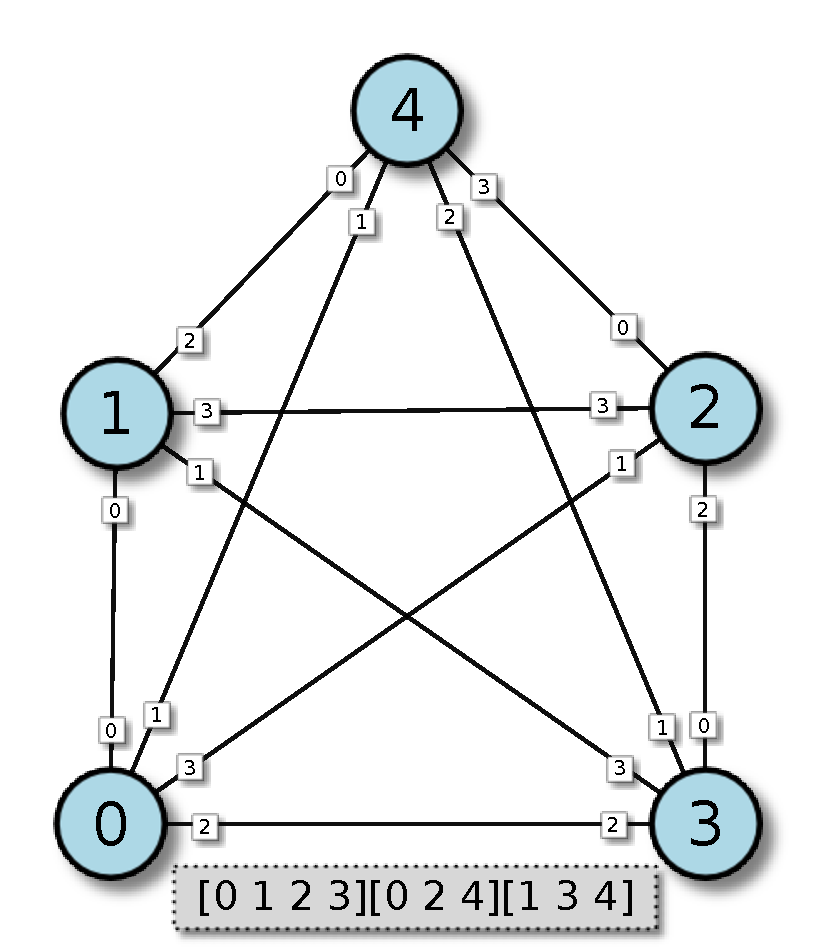
\includegraphics[width=.33\textwidth]{pics/K5-334-0123-024-134}\label{fig:334-rep}&
  \hspace{.33\textwidth} &
  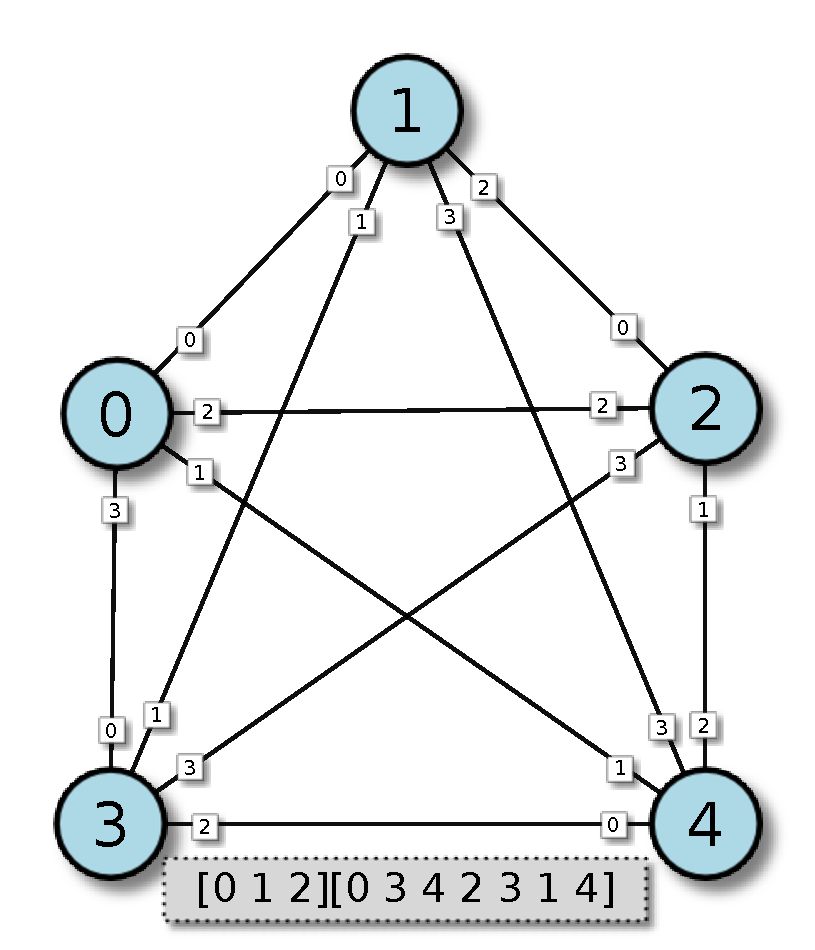
\includegraphics[width=.33\textwidth]{pics/K5-37-012-0342314}\label{fig:37-rep}  \\
  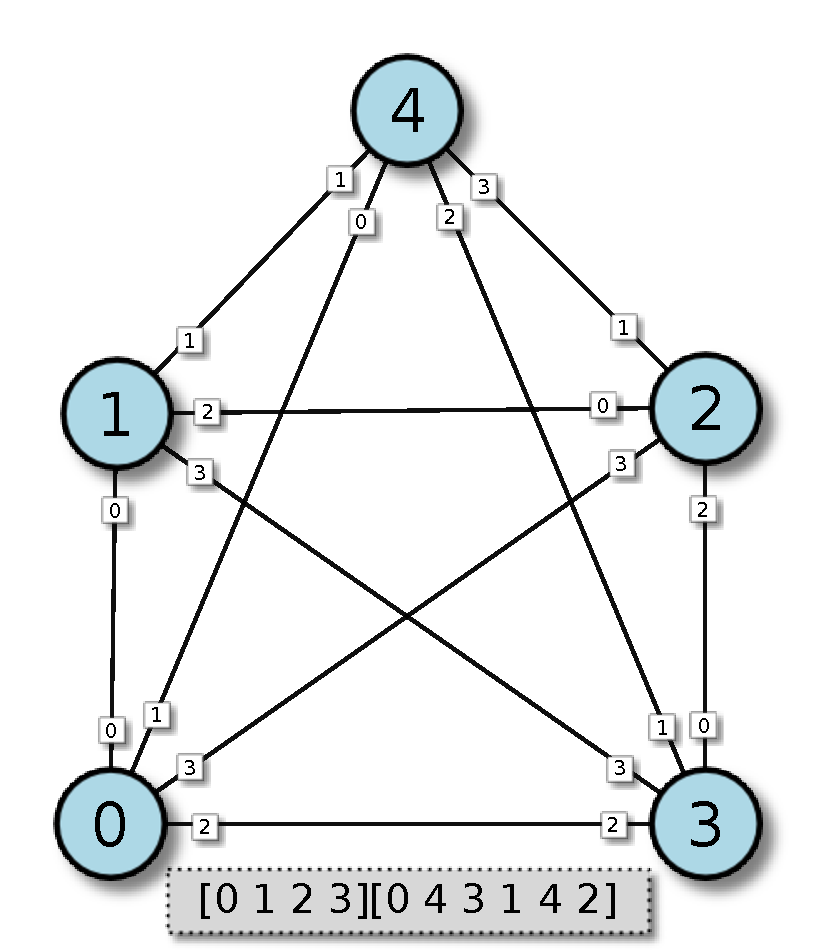
\includegraphics[width=.33\textwidth]{pics/K5-46-0123-043142}\label{fig:46-rep} &
  \hspace{.33\textwidth} &
  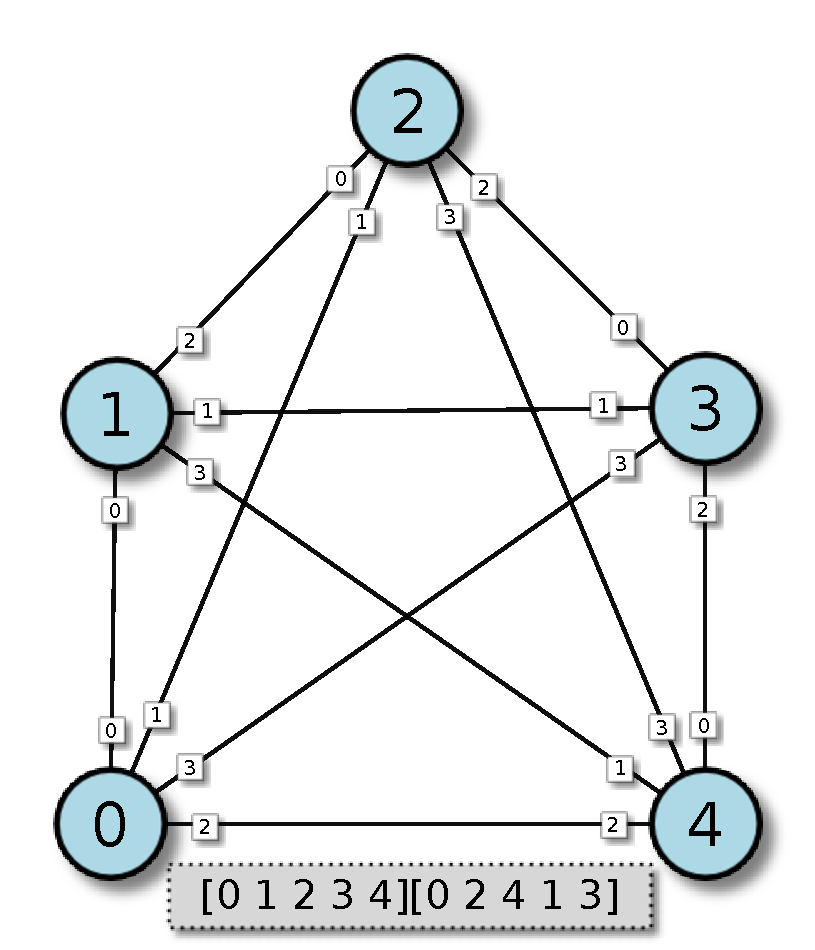
\includegraphics[width=.33\textwidth]{pics/K5-55-01234-02413}\label{fig:55-rep} \\
  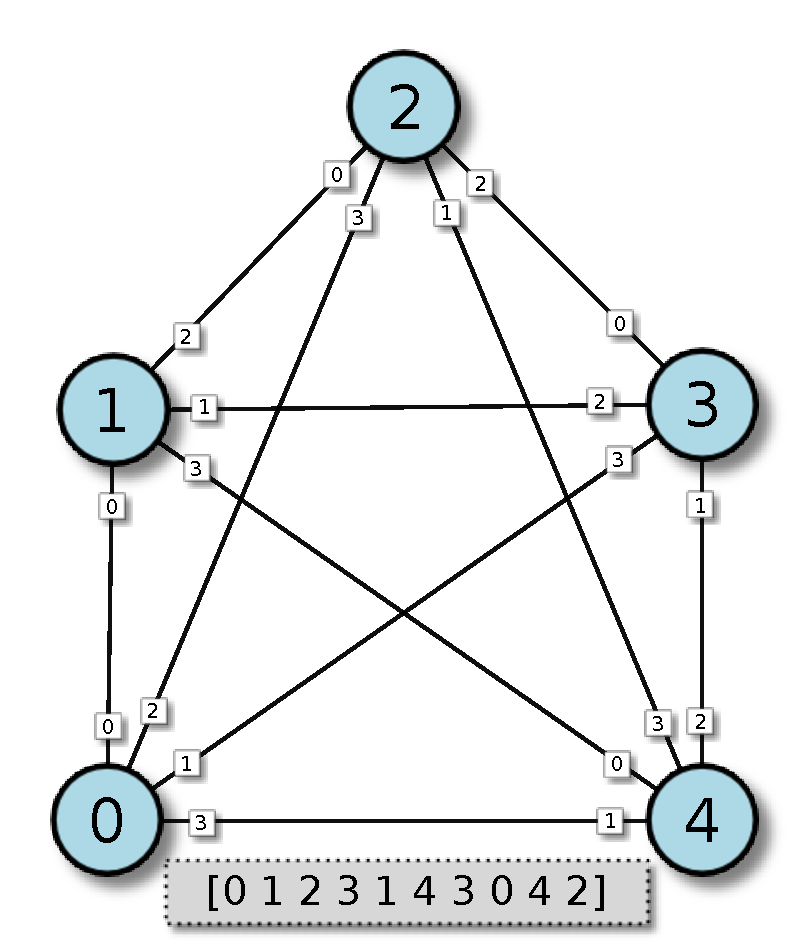
\includegraphics[width=.33\textwidth]{pics/K5-10_4d-0123143042}\label{fig:10_4d-rep}&
  \hspace{.33\textwidth} &
  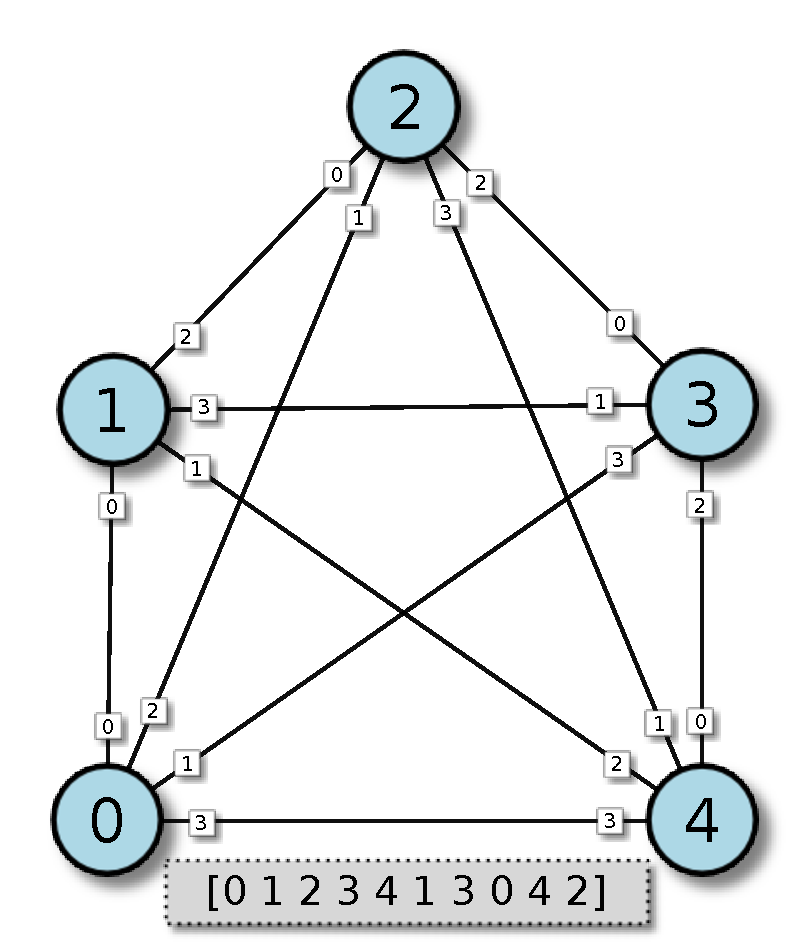
\includegraphics[width=.33\textwidth]{pics/K5-10_5d4s-0123413042}\label{fig:10_5d4s-rep} \\
  \ &
  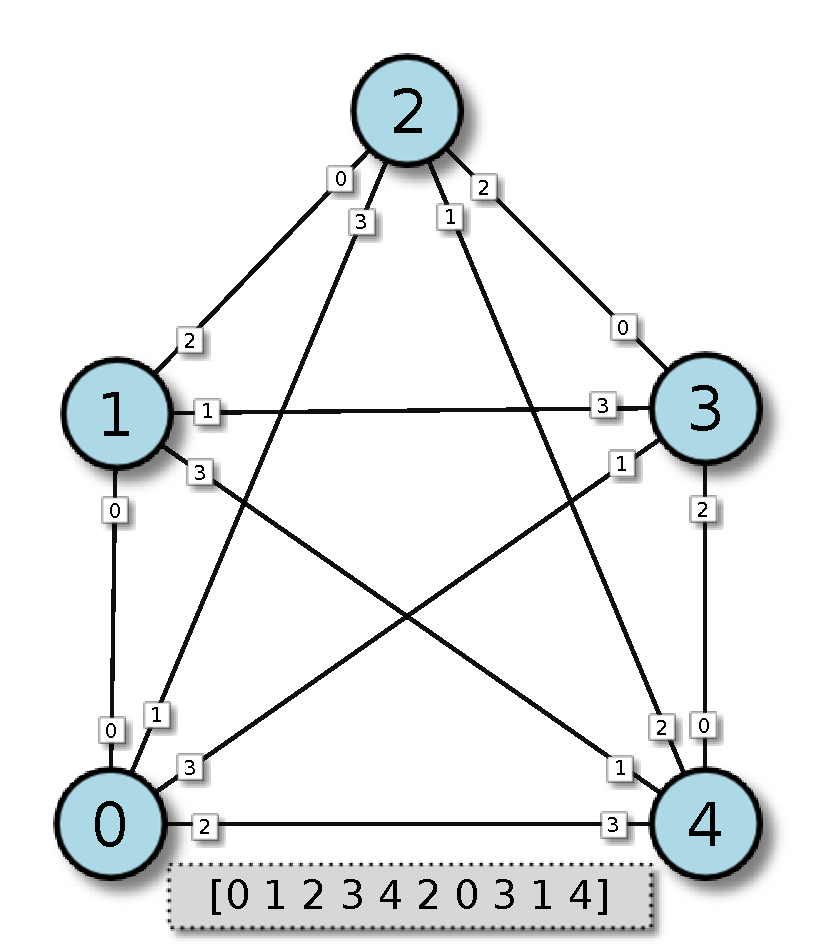
\includegraphics[width=.33\textwidth]{pics/K5-10_5d8s-0123420314}\label{fig:10_5d8s-rep} &
  \ 
\end{array}
$
\caption{Enumerations representing the seven major types of PCDs listed in Table~\ref{tbl:summary}.\label{fig:summary}} 
\end{minipage}
\end{figure}}

\begin{proposition}
  \label{prop:pcd_stab}
Table~\ref{tbl:summary} lists the stabilizer for each representative PCD and gives the size of it's orbit in $P$. 
\end{proposition}

\begin{proof}
  \label{pf:pcd_stab}
\ \\
\vspace{2ex}
\noindent
{\bf Case:} $3,3,4$ with representative $\pcd_{3,3,4} = \left(\left[0\ 1\ 2\ 3   \right], \left[0\ 2\ 4 \right], \left[ 1\ 3\ 4 \right]\right)$ 
\vspace{2ex}

\noindent
We will first show that $\left<\left(1\ 2\ 3 \right)(4),\  \left(1\ 2\right)\left(0\ 3 \right)\left(4\right)\right> \subseteq \stab{S_5}{ \pcd_{3,3,4} }$. We have that both $ \left( 0\ 1\ 2\ 3 \right)\left(4\right)$ and $\left(1\ 2\right)\left(0\ 3\right)\left(4\right)$ stabilize $\pcd_{3,3,4}$ since
\[ 
\acts{ \left( 0\ 1\ 2\ 3 \right)\left(4\right) }{\left[0\ 1\ 2\ 3 \right]  \left[0\ 2\ 4 \right] \left[ 1\ 3\ 4 \right]}  = \left[1\ 2\ 3\ 0 \right]\left[1\ 3\ 4 \right]\left[2\ 0\ 4 \right] \equiv \left[0\ 1\ 2\ 3 \right] \left[0\ 2\ 4\right] \left[ 1\ 3\ 4\right] 
\] and 
\[
\acts{\left(1\ 2\right)\left(0\ 3\right)\left(4\right)}{\left[0\ 1\ 2\ 3\right]\left[0\ 2\ 4\right]\left[1\ 3\ 4\right]}  = \left[3\ 2\ 1\ 0 \right]\left[3\ 1\ 4 \right]\left[2\ 0\ 4\right] \equiv \left[0\ 1\ 2\ 3 \right]\left[1\ 3\ 4 \right]\left[0\ 2\ 4 \right]
\] thus can conclude that $\left<\left(1\ 2\ 3 \right)(4),\  \left(1\ 2\right)\left(0\ 3 \right)\left(4\right)\right> \subseteq \stab{S_5}{ \pcd_{3,3,4} }$

For the reverse containment we let $\sigma \in \stab{S_5}{\pcd_{3,3,4}}$. Since $4$ is the only vertex which is not traversed within the $4$-circuit $\left[0\ 1\ 2\ 3\right]$ we have that $\sigma$ must fix it. Furthermore $\sigma$ must preserve the geometry of the $4$-circuit which implies that $\sigma$ must be in the dihedral subgroup $\left< \left(0\ 1\ 2\ 3\right),\left(0\ 3\right)\left(1\ 2\right) \right>$. Therefore in order to fix $\pcd_{3,3,4}$, $\sigma$ must be in $\left< \left( 0\ 1\ 2\ 3 \right)\left(4\right), \left(0\ 3 \right)\left(1\ 2\right)\left(4\right) \right>$ and the desired result has been reached. Furthermore since the stabilizer is a group of order $8$, we have that the orbit has $5!/8 = 15$ elements. 

\vspace{2ex}
\noindent
{\bf Case:} $3,7$ with representative $\pcd_{3,7} = \left(\left[0\ 1\  2 \right],\left[0\ 3\ 4\ 2\ 3\ 1\ 4 \right]\right) $
\vspace{2ex}

\noindent
We will first show that $\left<\left(1 \right)\left(3\ 4\right)\left(0\ 2\right)\right>$ is a subgroup of $\stab{S_5}{\pcd_{3,7}}$. We have that $\left(1 \right)\left(3\ 4\right)\left(0\ 2\right)$ stabilizes $\pcd_{3,7}$ since
\[     
\acts{\left(1\right)\left(3\ 4\right)\left(0\ 2\right)}{ \left[0\ 1\ 2\right]\left[0\ 3\ 4\ 2\ 3\ 1\ 4\right]} = \left[2\ 1\ 0\right]\left[2\ 4\ 3\ 0\ 4\ 1\ 3\right] \equiv \left[0\ 1\ 2\right]\left[0\ 3\ 4\ 2\ 3\ 1\ 4\right]
\] thus we can conclude that $\left< \left(1\right)\left(3\ 4\right)\left(0\ 2\right)\right> \subseteq \stab{S_5}{\pcd_{3,7}}$

To demonstrate the reverse containment, let $\sigma \in \stab{S_5}{\pcd_{3,7}}$.  We would like to show that $\sigma \in \left<\left(1\right)\left(3\ 4\right)\left(0\ 2\right)\right>$. The first thing to recognize is that since neither vertex $3$ nor $4$ are traversed within the $3$-circuit $[0\ 1\ 2]$ the permutation must preserve the partition $\{\{0,1,2\},\{3,4\}\}$. This implies that $\sigma$ either maps $3$ to $4$ or it fixes both. If $3$ is mapped to $4$ then $0$ must be mapped to $2$, and $2$ to $0$,  to preserve the sequence $2 \ 4 \ 3\ 0$ within the $7$-circuit. This then implies that $1$ must be fixed. Thus if $\sigma(3)=4$ then $\sigma = (1)(3\ 4)(0\ 2)$. Now suppose that $3$ and $4$ are fixed by $\sigma$. Once again to preserve sub-path $2\ 4\ 3\ 0$ within our $7$-circuit we must also fix $0$ and $2$. This then implies that we must also fix $1$ and therefore $\sigma$ fixes all vertices, so $\sigma = ()$. Thus we can conclude that $\sigma \in \left<(1)(3\ 4)(0\ 2) \right>$. Since our stabilizing group is of order $2$, the size of the orbit of $\pcd_{3,7}$ under the action of $S_5$ is $5!/2 = 60$.

\vspace{2ex}
\noindent
{\bf Case:} $4,6$ with representative $\pcd_{4,6} = \left(\left[0\ 1\ 2\ 3  \right],\left[0\ 4\ 3\ 1\ 4\ 2\right]\right)$
\vspace{2ex}

\noindent
We will first show that $\left< \left(0\ 1\ 2\ 3\right)\left(4\right)\right> \subseteq \stab{S_5}{\pcd_{4,6}}$. We have that $\left(0\ 1\ 2\ 3\right)\left(4\right)$ stabilizes $\pcd_{4,6}$ since
\[
\acts{\left(0\ 1\ 2\ 3\right)\left(4\right)}{\pcd_{4,6}} = \left[1\ 2\ 3\ 0\right]\left[1\ 4\ 0\ 2\ 4\ 3\right] \equiv \left[0\ 1\ 2\ 3\right]\left[0\ 4\ 1\ 3\ 4\ 2\right] 
\] thus $\left<\left(0\ 1\ 2\ 3\right)\left(4\right)\right> \subseteq \stab{S_5}{\pcd_{4,6}}$ which was the desired result.  

For the reverse containment let $\sigma \in \stab{S_5}{\pcd_{4,6}}$. Just as in the $3,3,4$ case it is necessary for $\sigma$ to fix the vertex $4$ and the stabilize the $4$-circuit $[0\ 1\ 2\ 3]$. Thus we can conclude that $\stab{S_5}{\pcd_{4,6}} \subseteq \left< (0\ 1\ 2\ 3)(4), (0\ 3)(1\ 2)(4) \right>$. However upon further inspection we have that the transposition $(0\ 3)(1\ 2)(4)$ does not fix the $7$-circuit. Thus we can conclude that $\stab{S_5}{\pcd_{4,6}} \subseteq \left< (0\ 1\ 2\ 3)(4) \right>$. Since the stabilizer of $\pcd_{4,6}$ is or order $4$ we can conclude, by the orbit-stabilizer theorem, that the size of this orbit is $5!/4 = 30$.

\vspace{2ex}
\noindent
{\bf Case:} $5,5$ with representative $\pcd_{5,5} = \left(\left[ 0\ 1\ 2\ 3\ 4 \right],\left[0\ 2\ 4\ 1\ 3 \right]\right)$.\\
\vspace{2ex}

\noindent
Again we would like to first show that $\left<  \left(0\ 1\ 2\ 3\ 4\right),\left(0\right)\left(1\ 2\ 4\ 3\right)\right> \subseteq \stab{S_5}{\pcd_{5,5}}$. Both $\left(0\ 1\ 2\ 3\ 4 \right)$ and $\left(0\right)\left(1\ 2\ 4\ 3\right)$ stabilize $\pcd_{5,5}$ since
\[
\acts{\left(0\right)\left(1\ 2\ 4\ 3\right)}{\pcd_{4,6}} = \left[0\ 2\ 4\ 1\ 3\right]\left[0\ 4\ 3\ 2\ 1\right] \equiv \left[0\ 2\ 4\ 1\ 3\right]\left[0\ 1\ 2\ 3\ 4\right]
\] 
and
\[
\acts{\left(0\ 1\ 2\ 3\ 4\right)}{\pcd_{5,5}} = \left[1\ 2\ 3\ 4\ 0\right]\left[1\ 3\ 0\ 2\ 4\right] \equiv \left[0\ 1\ 2\ 3\ 4\right]\left[0\ 2\ 4\ 1\ 3\right]
\] thus we can conclude that $\left<  \left(0\ 1\ 2\ 3\ 4\right),\left(0\right)\left(1\ 2\ 4\ 3\right)\right> \subseteq \stab{S_5}{\pcd_{5,5}}$

Now to show that we have the reverse containment let $\sigma \in \stab{S_5}{\pcd_{5,5}}$ and examine the image of the $5$ circuit $[0\ 1\  2\  3\  4]$ under the action provided by $\sigma$. Without loss of generality assume that $\sigma(0) = 0$, if not then apply the permutation $(0\ 1\ 2\ 3\ 4)$ until this is true. Assuming that $\sigma(0) = 0$, we then only have $4$ possibilities for the image of $[0\ 1\ 2\ 3\ 4]$. We must map $\left[ 0\ 1\ 2\ 3\ 4\right]$ to either $\left[0 \ 1\ 2\ 3\ 4 \right]$, $\left[ 0 \ 2\ 4\ 1\ 3 \right]$, $\left[ 0\ 3\ 1\ 4\ 2\right]$, or $[0\ 4\ 3\ 2\ 1]$. This then implies that $\sigma$ is either $\left(\right)$,  $(0)(1\ 2\ 4\ 3)$,  $(0)(1\ 3\ 4\ 2) = ((0)(1\ 2\ 4\ 3))^{-1} $, or $ (0)(1\ 4)(2\ 3) = \left((0)(1\ 2\ 4\ 3 )\right)^2$. Which implies that $\sigma \in \left< (0\ 1\ 2\ 3\ 4), (0)(1\ 2\ 4\ 3) \right> $. Therefore we can conclude that $\stab{S_5}{\pcd_{5,5}} \subseteq \left<  \left(0\ 1\ 2\ 3\ 4\right),\left(0\right)\left(1\ 2\ 4\ 3\right)\right>$ and since the set of stabilizing permutations is of order $20$, than the orbit has $\frac{5!}{20} = 6 $ elements \\

The following three cases deal with PCDs which all have $10$ as their signature. What will distinguish one circuit from the other is a difference in how many unique vertices are traversed before repeating. We will say that a PCD is {\em  $n$-distinct} if the maximum number of unique vertices traversed before duplicates is equal to $n$. We will call the starting vertex of a distinct sequence a {\em start}. If the unique sequence appears while reading the listing from left-to-right will call this a {\em forward sequence}, with the starting vertex being a {\em forward start}, while if the sequence occurs from right-to-left we say that this a {\em backward sequence}, and a {\em backward start} respectively. For example, the PCD $\left[0\ 1\ 2\ 3\ 4\ 0\ 2\ 4\ 1\ 3 \right]$ is a $5$-distinct circuit as the $5$ vertices $0\ 1\ 2\ 3\ 4$ are traversed in forward order. Also traversed in forward order are the sequences 
\begin{itemize}
\item $1\ 2\ 3\ 4\ 0$,
\item $0\ 2\ 4\ 1\ 3$, and 
\item $2\ 4\ 1\ 3\ 0$
\end{itemize}
\noindent
and in the backward order
\begin{itemize}
\item $3\ 1\ 4\ 2\ 0$, 
\item $0\ 4\ 3\ 2\ 1$,
\item $4\ 3\ 2\ 1\ 0$, and
\item $0\ 3\ 1\ 4\ 2$.
\end{itemize}
\noindent
Which can be written in the more compact notation $\left[\overline{\underline{0}}\ \underline{1}\ 2\ 3\ \overline{4}\ \overline{\underline{0}}\ \underline{2}\ 4\ 1\ \overline{3} \right]$ where an overbar on a vertex denotes that it is a backward start and underline denotes that a vertex is a forward start.

The number of starts and the maximum number of distinct vertices will be a defining characteristic of the PCDs with signature $10$. This is due to the fact that $S_5$ respects this property, as every bijection of $\left\{0\ 1\ 2\ 3\ 4\right\}$ into itself will send a $n$ distinct sequence to another one.

\vspace{2ex}
\noindent
{\bf Case:} $10$ with $4$-distinct and representative $\pcd_{10-4d} = \left(\left[\underline{0}\ \overline{1}\ \underline{2}\ \overline{3}\ \underline{1}\ \overline{4}\ \underline{3}\ \overline{0}\ \underline{4}\ \overline{2} \right]\right)$
\vspace{2ex}

\noindent
We will first show that $\left< \left(0\ 2\ 1\ 3\ 4\right),\left(3\right)\left(0\ 2\right)\left(1\ 4\right)\right> \subseteq \stab{S_5}{\pcd_{10-4d}}$. We have that both $\left(0\ 2\ 1\ 3\ 4\right)$ and $\left(3\right)\left(0\ 2\right)\left(1\ 4\right)$ fix $\pcd_{10-4d}$ since
\[
\acts{\left(0\ 2\ 1\ 3\ 4\right)}{\pcd_{10-4d}} = \left(\left[2\ 3\ 1\ 4\ 3\ 0\ 4\ 2\ 0\ 1\right] \equiv \left[0\ 1\ 2\ 3\ 1\ 4\ 3\ 0\ 4\ 2\right]\right)
\] and
\[
\acts{\left(3\right)\left(0\ 2\right)\left(1\ 4\right)}{\pcd_{10-4d}} = \left[2\ 4\ 0\ 3\ 4\ 1\ 3\ 2\ 1\ 0 \right] \equiv \left[0\ 1\ 2\ 3\ 1\ 4\ 3\ 0\ 4\ 2\right]
\] thus we can conclude that $\left<\left(0\ 2\ 1\ 3\ 4\right),\left(3\right)\left(0\ 2\right)\left(1\ 4\right)\right> \subseteq \stab{S_5}{\pcd_{10-4d}}$.  


To show the reverse containment we let $\sigma \in \stab{S_5}{\pcd_{10-4d}}$. $\pcd_{10-4d}$ is a $4$-distinct parity circuit with $10$ different $4$-distinct sequences, thus every vertex of $K_5$ is a start of exactly one forward and backward sequence. Using the notation discussed earlier, $\pcd_{10-4d} = [\underline{0}\  \overline{1}\  \underline{2}\  \overline{3}\  \underline{1}\  \overline{4}\  \underline{3}\  \overline{0}\  \underline{4}\ \overline{2} ]$. $\sigma$ will be determined completely by where it sends the sequence $0\ 1\ 2\ 3$. Recalling that $\sigma$ must send this $4$-distinct path to another, there are $10$ possible permutations, all of which are listed in Table~\ref{tbl:4dpcdstab} and all of these can be shown to be contained in $\left< \left(0\ 2\ 1\ 3\ 4\right),\left(3\right)\left(0\ 2\right)\left(1\ 4\right)\right>$. 

\begin{table}[h]
  \caption{Stabilizing Group of PCD $\left([0\ 1\ 2\ 3\ 1\ 4\ 3\ 0\ 4\ 2]\right)$}
  \label{tbl:4dpcdstab}
  \vspace{1ex}
  \centering
  \begin{tabular}[h!]{ | c | c | c | c| c | c|}
\hline
Forward & $[0\ 1\ 2\ 3]$& $[1\ 4\ 3\ 0]$ & $[2\ 3\ 1\ 4]$ & $[3\ 0\ 4\ 2]$ & $[4\ 2 \ 0\ 1]$ \\
\hline
Backward & $[0\ 3\ 4\ 1]$& $[1\ 0\ 2\ 4]$  & $[2\ 4\ 0\ 3]$ & $[3\ 2\ 1\ 0]$ & $[4\ 1\ 3\ 2]$ \\
\hline
 $\sigma$& $()$ & $(0\ 1\ 4\ 2\ 3)$ &   $(0\ 2\ 1\ 3\ 4)$& $(0\ 3\ 2\ 4\ 1)$ & $(0\ 4\ 3\ 1\ 2)$   \\
        & $(0)(1\ 3)(2\ 4)$  & $(2)(0\ 1)(3\ 4)$  & $(3)(0\ 2)(1\ 4)$ & $(4)(0\ 3)(2\ 1)$ &$(1)(0\ 4)(2\ 3)$  \\
\hline
  \end{tabular}
\end{table}

\noindent
Since the set of stabilizing permutations is of size $10$ we have that the orbit has $5!/10 = 12$ elements.

\vspace{2ex}
\noindent
{\bf Case:} $10$ with $5$-distinct and $4$ starts with representative $\pcd_{10-5d4s} = \left(\left[\underline{0}\ 1\ 2\ 3\ \overline{4}\ \underline{1}\ 3\ 0\ 4\ \overline{2} \right] \right)$.
\vspace{2ex}

\noindent
We will first show that $\left<\left(3\right)\left(0\ 2\right)\left(1\ 4\right)\right> \subseteq \stab{S_5}{\pcd_{10-5d4s}}$. We have that $\left(3\right)\left(0\ 2\right)\left(1\ 4\right)$ stabilizes $\pcd_{10-5d4s}$ since
\[
\acts{\left(3\right)\left(0\ 2\right)\left(1\ 4\right)}{\pcd_{10-4d}} = \left[2\ 4\ 0\ 3\ 1\ 4\ 3\ 2\ 1\ 0\right] \equiv \left[0\ 1\ 2\ 3\ 4\ 1\ 3\ 0\ 4\ 2 \right]
\]  thus we can conclude that $\left<\left(3\right)\left(0\ 2\right)\left(1\ 4\right)\right> \subseteq \stab{S_5}{\pcd_{10-5d4s}}$ as desired. 

For the reverse containment, let $\sigma \in \stab{S_5}{\pcd_{10-5d4s}}$. $\pcd_{10-5d4s}$ is a $5$-distinct PCD with $4$ starts, two forward and two backward, listed as follows $[\underline{0}\ 1\ 2\ 3\ \overline{4}\ \underline{1}\ 3\ 0 \ 4\ \overline{2}]$. Then $\sigma$ will be completely determined by where it sends the $5$-distinct sequence $0\ 1\ 2\ 3\ 4$. There are only three options as to where to send this sequence, either $2\ 4\ 0\ 3\ 1$, $2\ 4\ 0 \ 3\ 1$, or $4\ 3\ 2\ 1\ 0$. Now since $3$ is the only vertex which doesn't start a $5$ distinct sequence it must be fixed by $\sigma$. Thus $\sigma$ cannot send $0\ 1\ 2\ 3\ 4$ to either $1\ 3\ 0\ 4\ 2$ or $4\ 3\ 2\ 1\ 0$.  This implies that $\sigma$ is either $(0\ 2)(1\ 4)(3)$  or the identity permutation. Thus $\sigma \in \left<\left(3\right)\left(0\ 2\right)\left(1\ 4\right)\right>$.  Therefore since the set of stabilizing permutations has $2$ elements we have that the size of the orbit is $5!/2 = 60$

\vspace{2ex}
\noindent
{\bf Case:} $10$ with $5$-distinct and $8$ starts with representative $\pcd_{10-5d8s}=\left( \left[0\ 1\ 2\ 3\ 4\ 2\ 0\ 3\ 1\ 4\right]\right)$.
\vspace{2ex}

\noindent
We will begin by showing that $\left< \left(0\ 3\right)\left(1\ 2\right)\left(4\right)\right> \subseteq \stab{S_5}{\pcd_{10-5d8s}}$. We have that $\left(0\ 3\right)\left(1\ 2\right)\left(4\right)$ stabilizes $\pcd_{10-5d8s}$ since
\[
\acts{\left(0\ 3\right)\left(1\ 2\right)\left(4\right)}{\pcd_{10-5d8s}} = \left[3\ 2\ 1\ 0\ 4\ 1\ 3\ 0\ 2\ 4\right] \equiv \left[0\ 1\ 2\ 3\ 4\ 2\ 0\ 3\ 1\ 4\right]
\]  thus we can conclude that $\left<\left(0\ 3\right)\left(1\ 2\right)\left(4\right)\right> \subseteq \stab{S_5}{\pcd_{10-4d}}$ as desired.

For the reverse containment let $\sigma \in \stab{S_5}{\pcd_{10-5d8s}}$. $\pcd_{10-5d8s}$ is a $5$-distinct PCD with $8$ starts, four forward and four backward, listed as follows $[\underline{0}\ 1\ 2\ \overline{3}\ \underline{\overline{4}}\ \underline{2}\ 0\ 3\ \overline{1}\ \underline{\overline{4}}]$. Just as in the last case a stabilizing permutation $\sigma$ is entirely determined by where it sends the $5$-distinct sequence $0\ 1\ 2\ 3\ 4$. Now since $4$ is the only vertex which is both a forward and a backward start we have that it must be fixed by $\sigma$. Thus $0 \ 1\ 2\ 3\ 4$ can only be sent to $5$-distinct sequences that end with vertex $4$. This implies that there are only $4$ possible images, $0\ 1\ 2\ 3\ 4$, $2\ 0\ 3\ 1\ 4$, $3\ 2\ 1\ 0\ 4$ and $1\ 3\ 0\ 2\ 4$. Of those four, only $0\ 1\ 2\ 3\ 4$ and $3\ 2\ 1\ 0\ 4$ are images of a stabilizing permutation. Therefore we can conclude that $\sigma$ is either the identity or equal to $(0\ 3)(1\ 2)(4)$. Thus $\stab{S_5}{\pcd_{10-5d8s}} \subseteq \left<(0\ 3)(1\ 2)(4) \right>$. Moreover, since the set of stabilizing permutations is of size $2$ we have that the orbit has $5!/2 = 60$ elements. 
\end{proof}

\section{Connections to the Zig-Zag and Replacement Products}
\label{sec:pcd_zz_rr}


The previous portions of this chapter have been dedicated to counting and classifying the parity circuit decompositions of $K_5$. In this section we would like to make explicit the connection between the parity circuits and the zig-zag and replacement products defined in Chapter~\ref{chapt:old_zz}.

\subsection{PCDs and the Replacement Product}
\label{sec:cloud-circ-repl}


\begin{theorem}
  \label{thm:replacement_cats}
$K_5 \replacement C_4$  is equal to, modulo {\em replacement product isomorphism} to one of the following
\begin{itemize}
\item A $3,3,4$ circuit replacement product.
\item A $3,7$ circuit replacement product. 
\item A $4,6$ circuit replacement product.
\item A $5,5$ circuit replacement product.
\item A $10$ circuit with $4$-distinct replacement product.
\item A $10$ circuit with $5$-distinct (with 4 starts) replacement product.
\item A $10$ circuit with $5$-distinct (with 8 starts) replacement product. 
\end{itemize}
All of which are depicted in Figure~\ref{fig:K5rrC4all}.
\end{theorem}

\afterpage{\clearpage
\begin{figure}[H]
\centering
\begin{minipage}{.95\textwidth}
$
\begin{array}[h]{ccccc}
  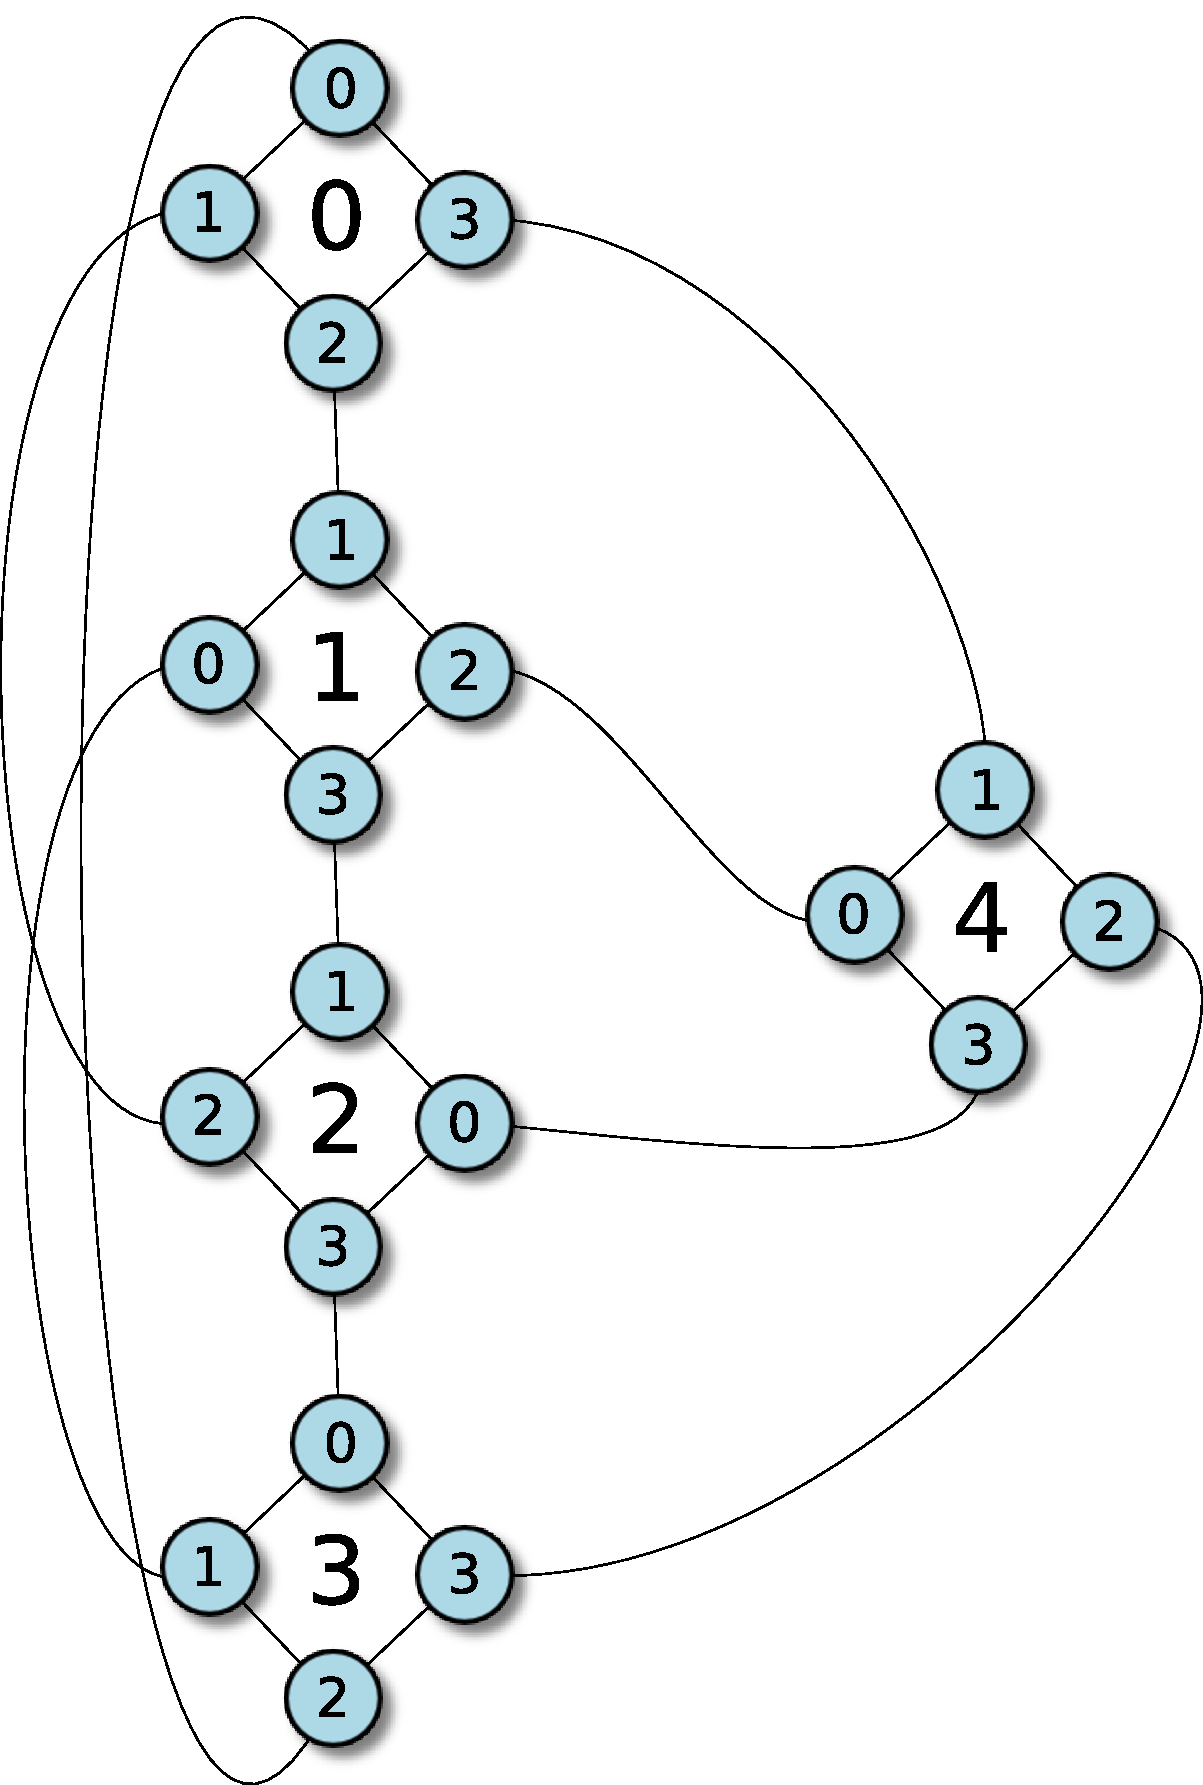
\includegraphics[height=.24\textheight]{pics/3-3-4-replacement-0123-024-134}\label{fig:repl-334} &
  &
  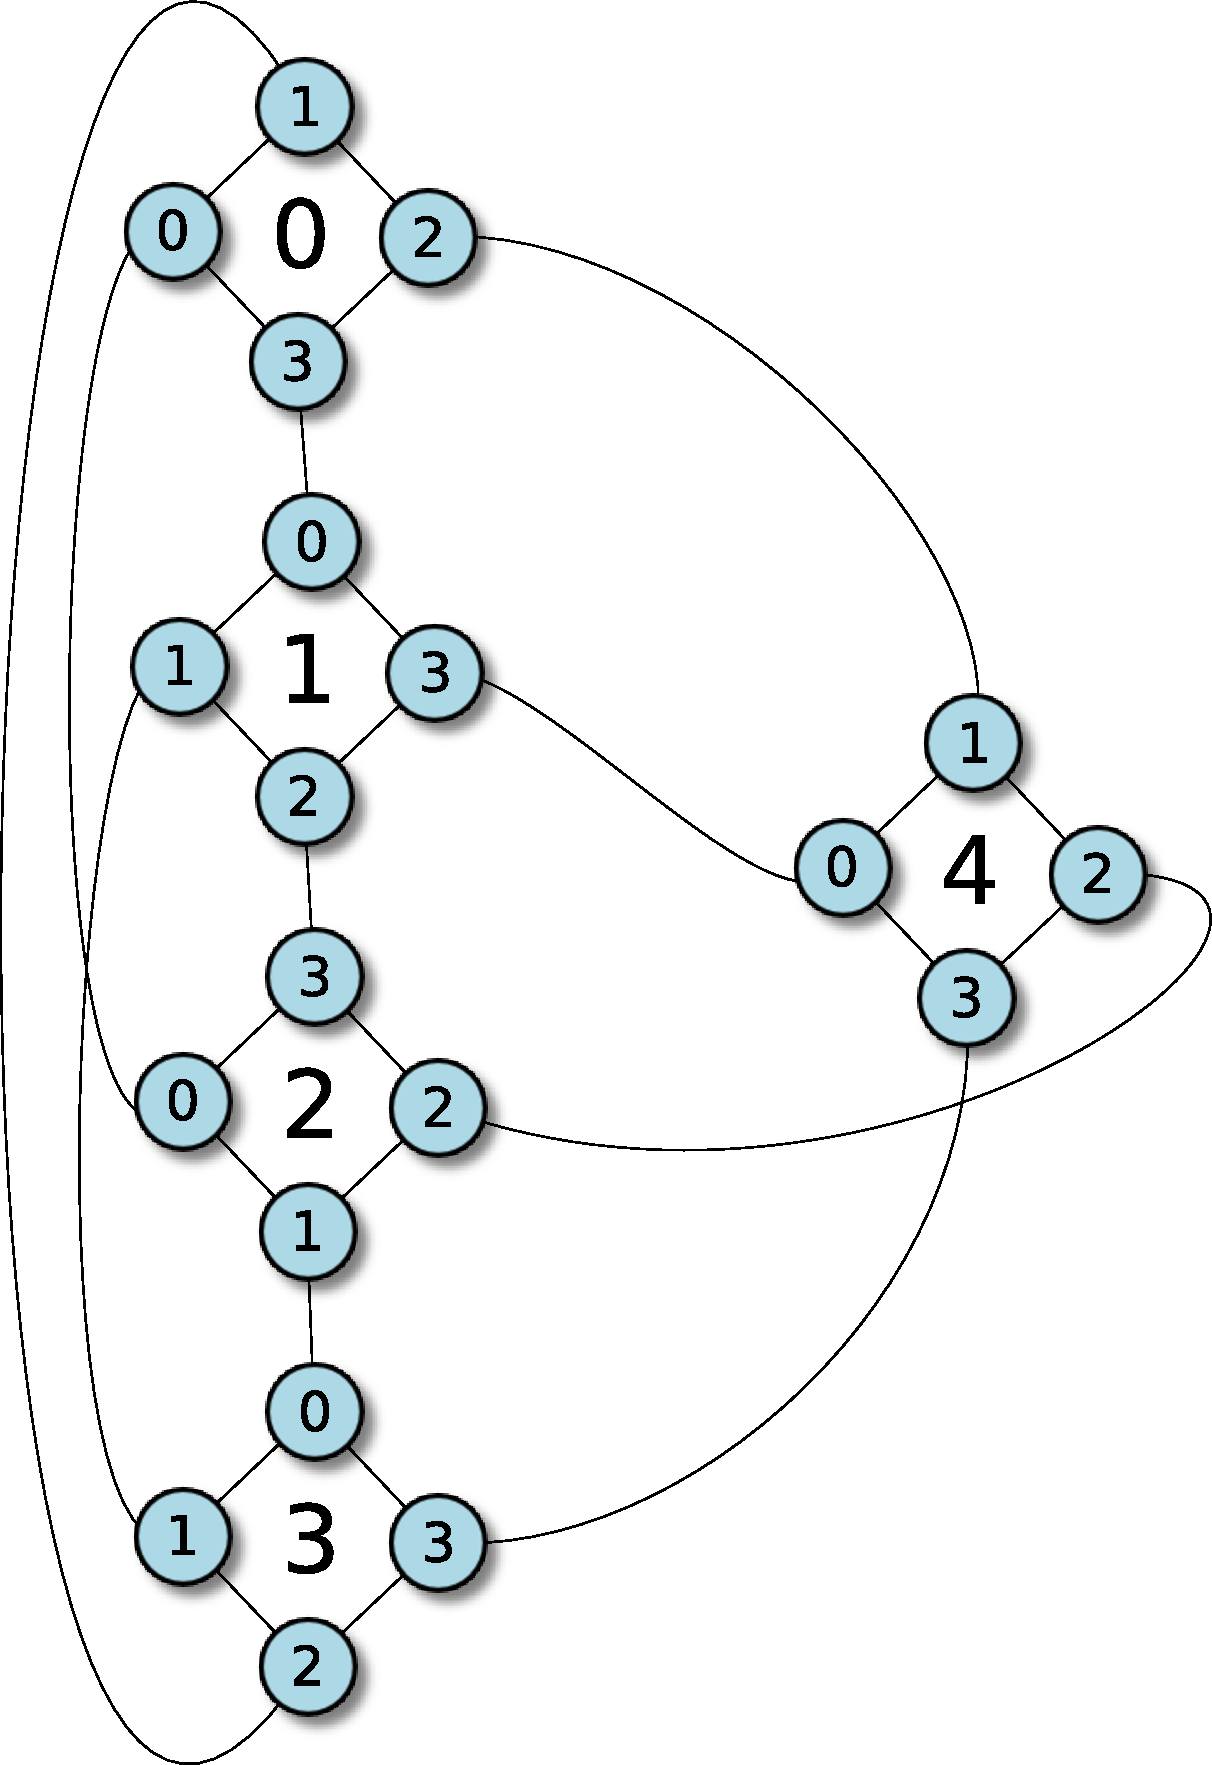
\includegraphics[width=.24\textwidth]{pics/4-6-replacement-0123-043142}\label{fig:repl-46} &
  &
  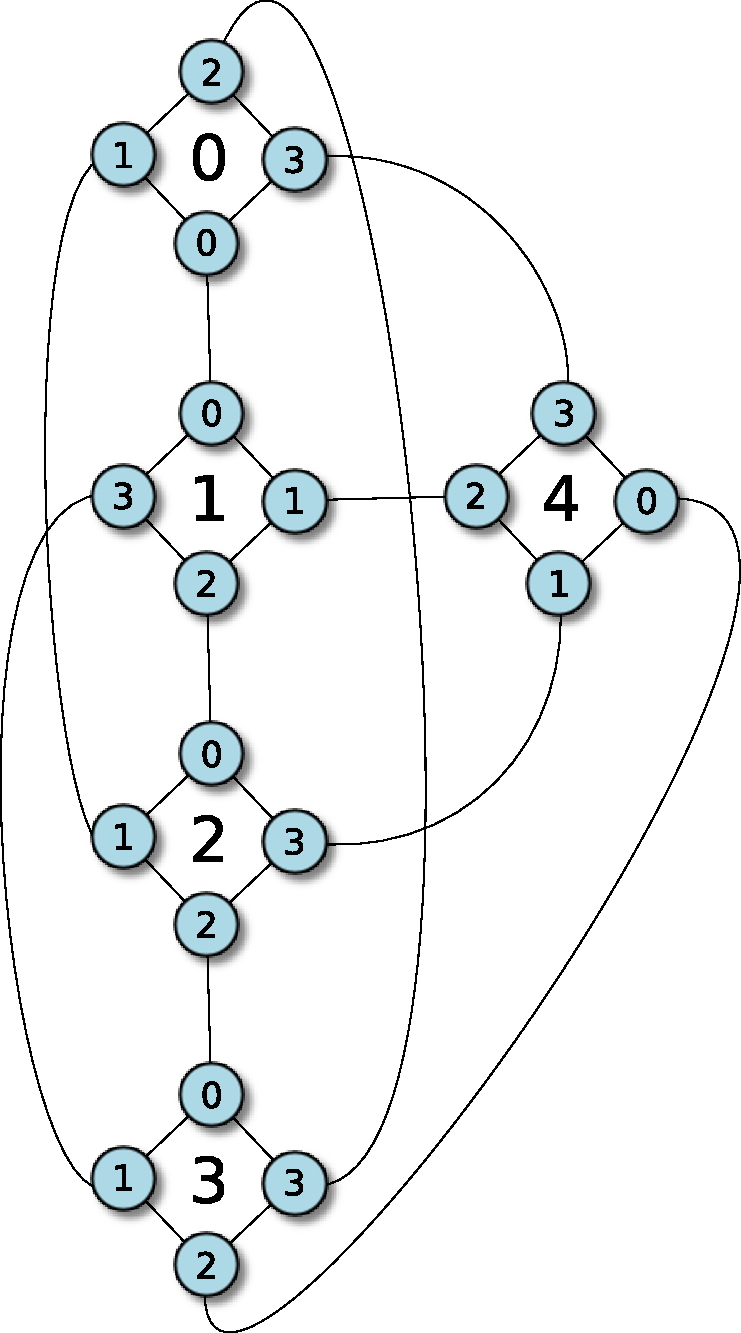
\includegraphics[height=.24\textheight]{pics/3-7-replacement-024-0123413}\label{fig:repl-37} \\
  \vspace{.05\textheight} \\
  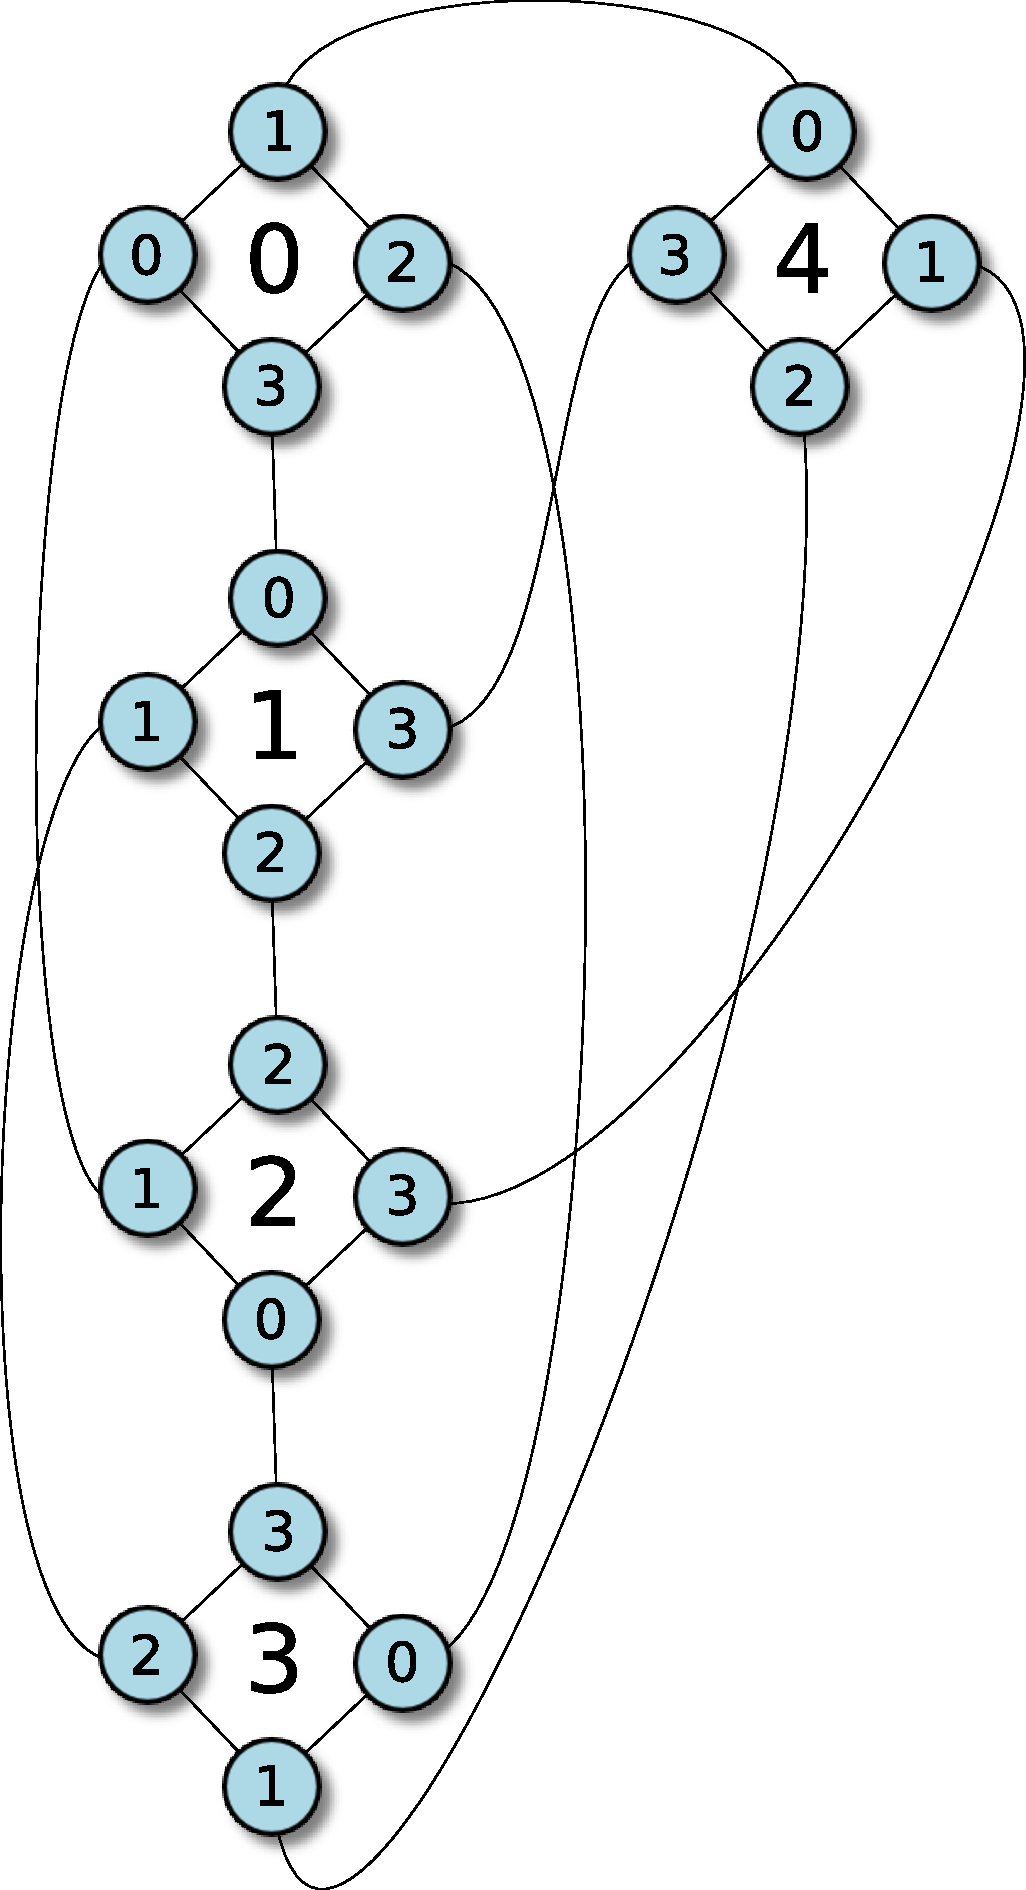
\includegraphics[height=.24\textheight]{pics/5-5-replacement-01234-02413}\label{fig:repl-55} &
  &
  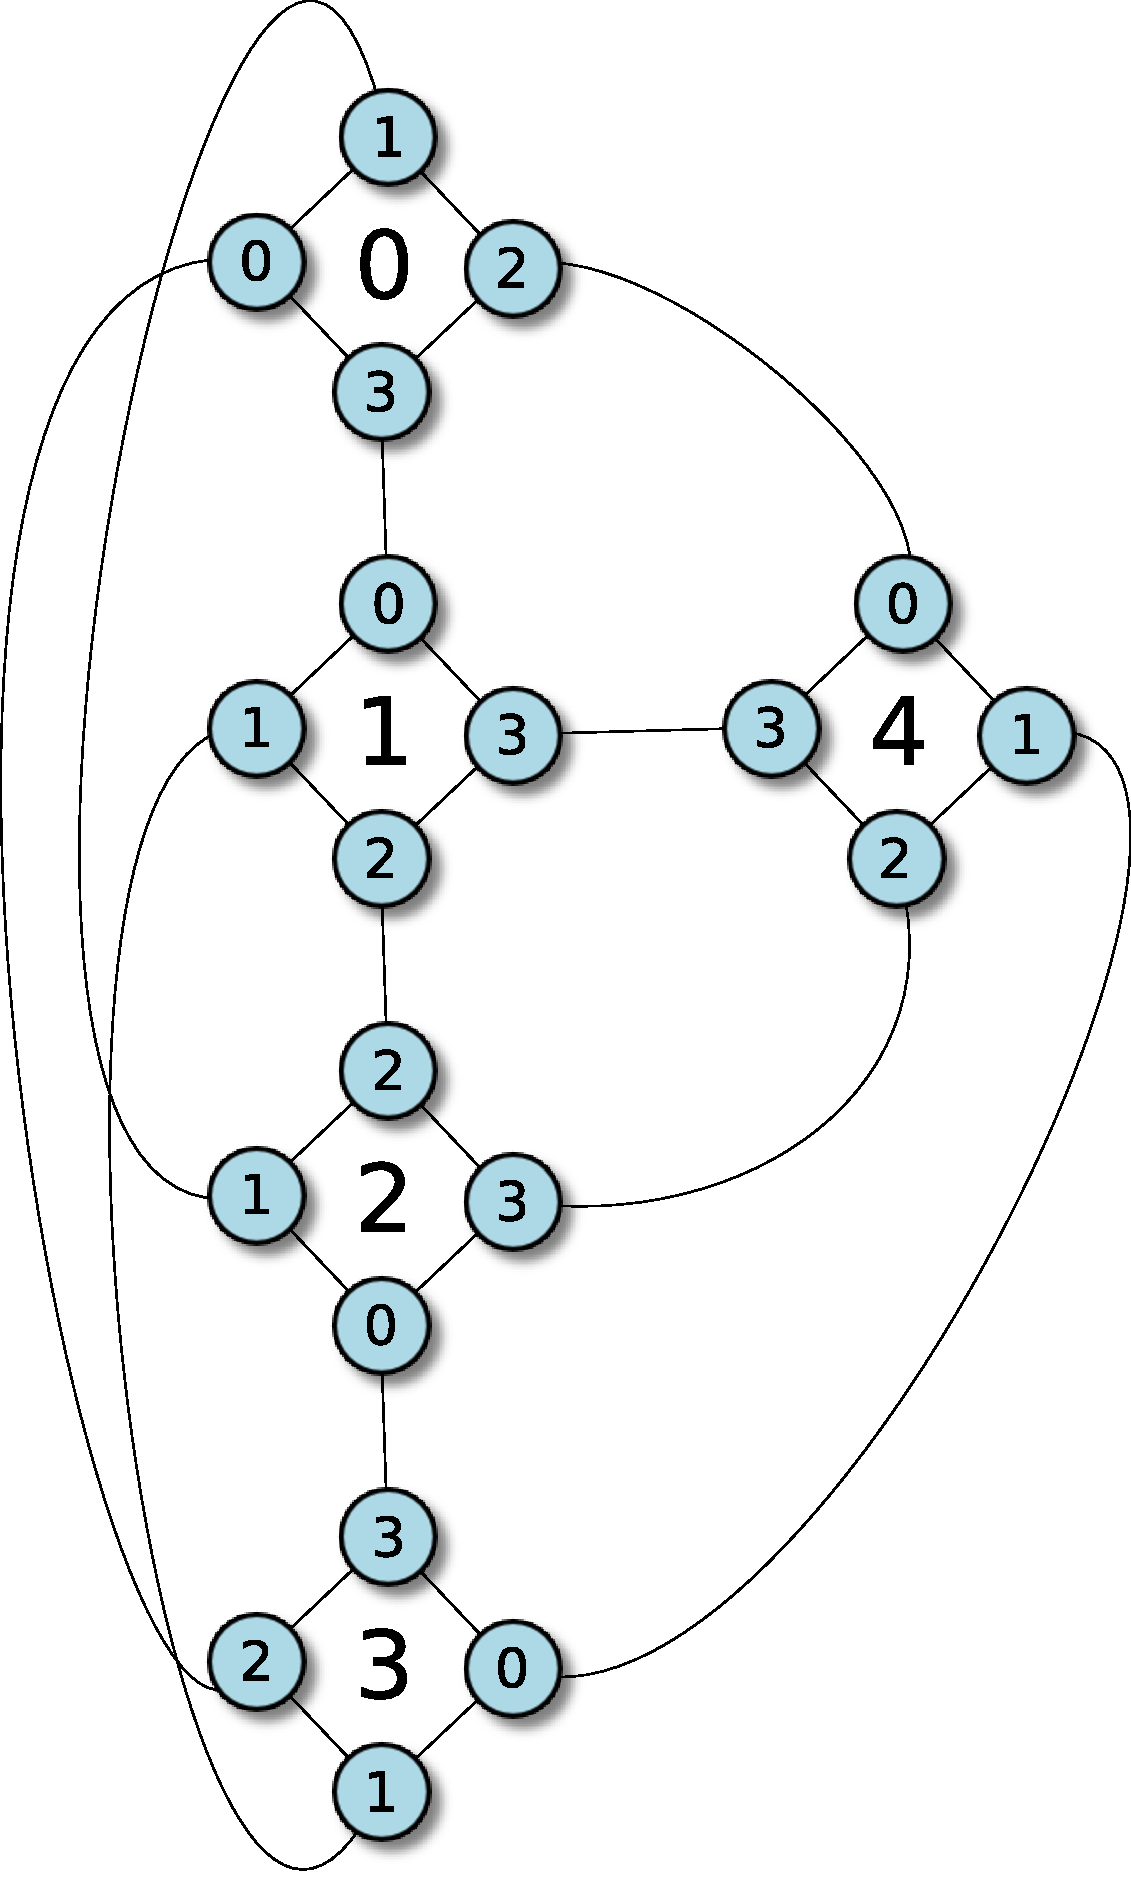
\includegraphics[height=.24\textheight]{pics/10_4d-replacement-0123143042}\label{fig:repl-10_4d}&
  &
  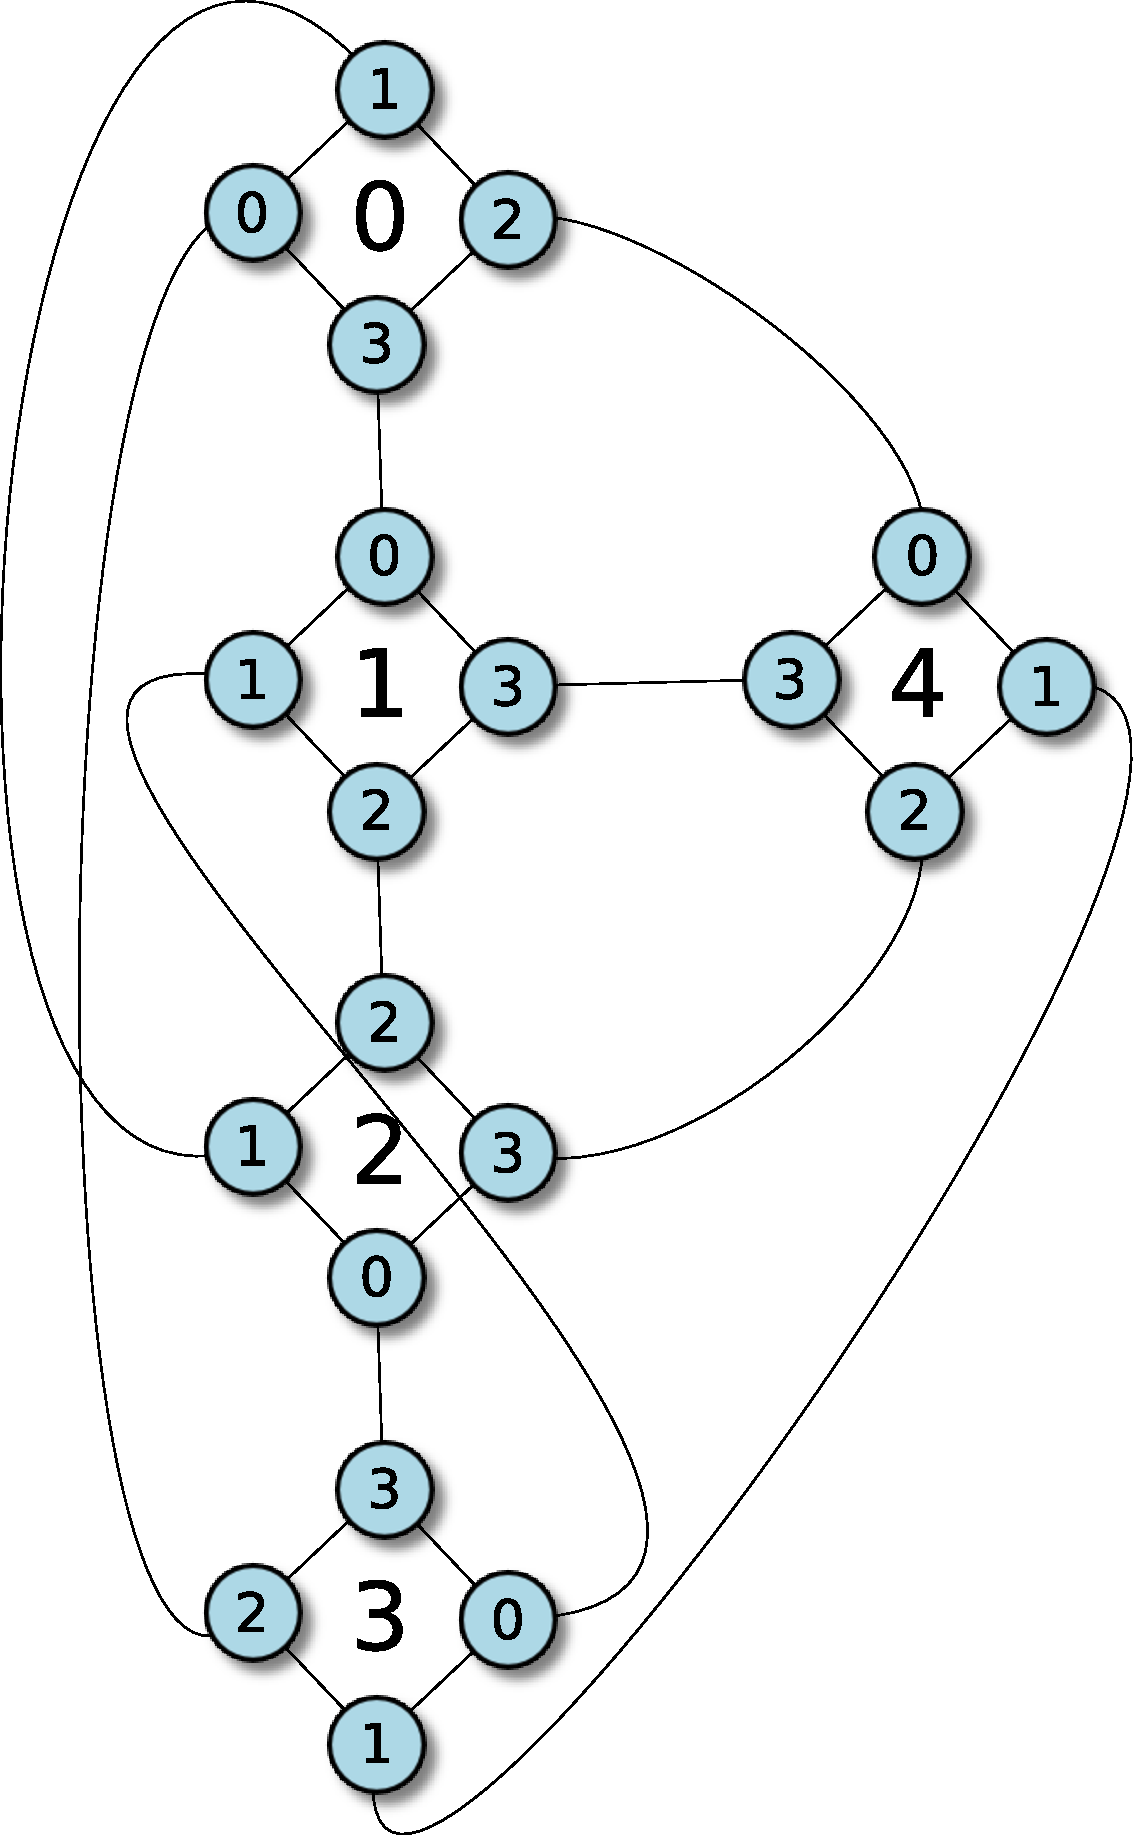
\includegraphics[height=.24\textheight]{pics/10_5d4s-replacement-0123413042}\label{fig:repl-10_5d4s}  \\
  \vspace{.05\textheight} \\
  \hspace{.30\textwidth} &
  &
  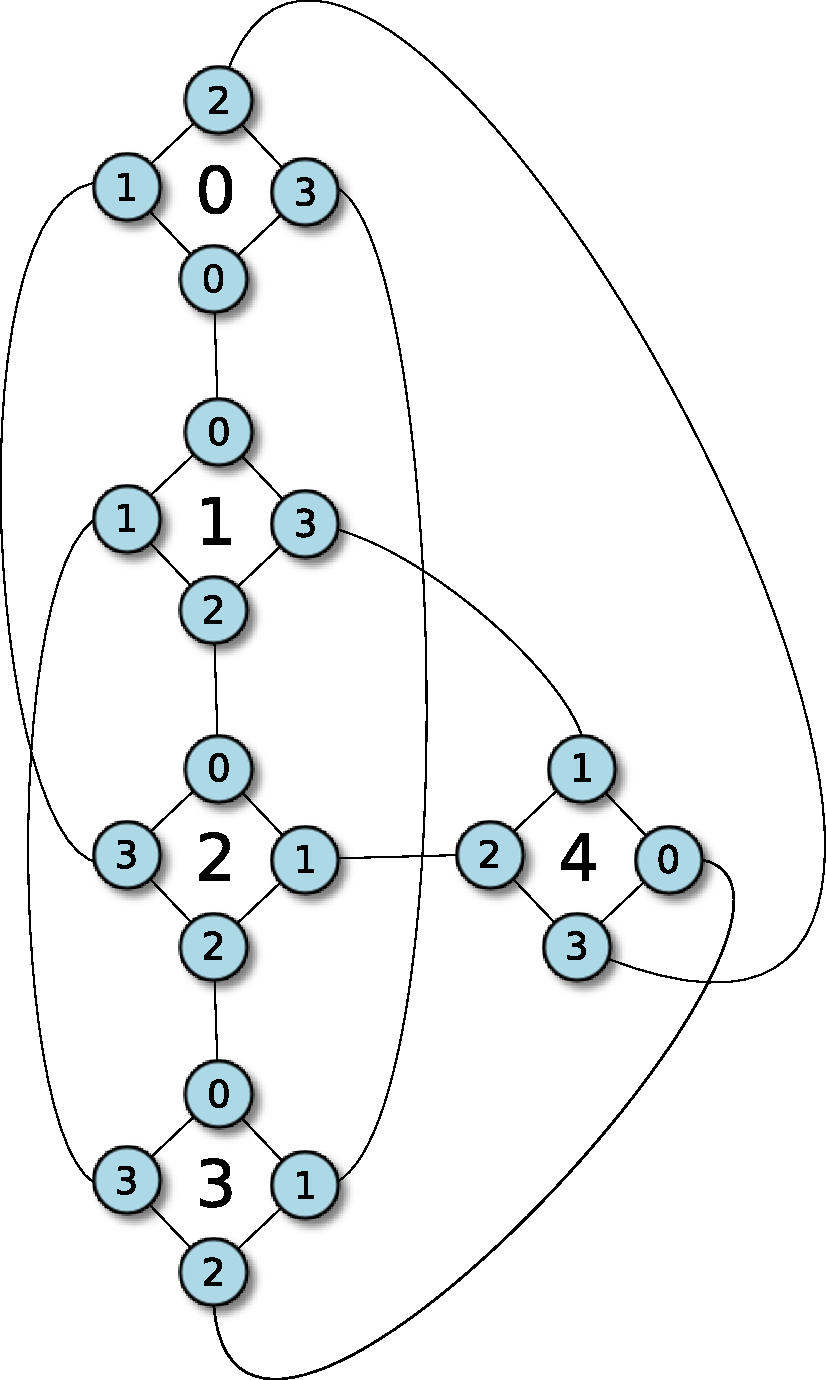
\includegraphics[height=.24\textheight]{pics/10_5d8s-replacement-0123420314}\label{fig:repl-10_5d8s}&
  &
  \hspace{.30\textwidth}\\
\end{array}
$
\caption{Representatives of the $7$ distinct classes of $K_5 \protect \replacement C_4$.\label{fig:K5rrC4all}}
\end{minipage}
\end{figure}}


\begin{lemma}
 Let $K_5$ have enumeration $\Enum$ let $\enum_{u}(v) = \enum_{v}(u) + 2 \bmod{4}$ for $u,v, w \in \vertS{K_5}$. $g(\enum_{u}(v)) = g(\enum_{u}(w)) + 2 \bmod{4}$ if and only if $g \in D_4$. 
\end{lemma}
\begin{proof}

Let $D_4 = \left< (0\ 1\ 2\ 3), (1\ 2)(0\ 3) \right>$ and note that $g$ is as above if and only if $g$ preserves the partition $\left\{ \left\{0, 2\right\}, \left\{1, 3\right\} \right\}$. We have demonstrated earlier that $g$ has to be in $D_4$. 
\end{proof}

\begin{proposition}
  \label{prop:pc_rpiso}
Let $\Enum$ and $\Enum^{\prime}$ be two enumerations of $K_5$ such that there exists and rp-isomorphism $F:K_5 \replacement C_4 \longrightarrow K_5 \replacement^{\prime} C_4$. Then then for each $\Enum$-{parity-circuit} $\ppath$, $\acts{F}{\ppath}$ is a $\Enum^{\prime}$-{parity-circuit}.
\end{proposition}


\begin{proof}

Let $\ppath = \left[ u_1\ u_2\ \cdots\ u_k\right]$. Then we would like to show that $\acts{F}{\ppath} = \left[ f(u_1)\ f(u_2)\ \cdots\ f(u_k)\right]$ is a $\Enum^{\prime}$-{parity-circuit}. We have that for each $i$, modulo $k$, that \[ \enum_{u_i}(u_{i-1}) = \enum_{u_i}(u_{i-1}) + 2 \bmod{4}     \]. Now since $g_{u_i} \in \Aut(C_4) = D_4$ preserves the partition $\left\{ \left\{0,2 \right\}  , \left\{1,3  \right\}  \right\}$ we have that \[    g_{u_i}(\enum_{u_i}(u_{i-1})) = g_{u_i}(\enum_{u_i}(u_{i-1})) + 2 \bmod{4}             \] which by the properties of rp-isomorphisms implies that $\enum^{\prime}_{f(u_{i})}(f(u_{i-1})) = \enum^{\prime}_{f(u_i)}(f(u_{i+1})) + 2 \bmod{4}$ for all $i$, modulo $k$. Thus we can conclude that $\acts{F}{\ppath}$ is a $\Enum^{\prime}$-{parity-circuit}.  
\end{proof}

\begin{corollary}
\label{cor:pcd_rpiso}
With the notation of Proposition~\ref{prop:pc_rpiso}. $\acts{F}{\pcd}$ is a $\Enum^{\prime}$-{parity circuit decomposition} whenever $\pcd$ is a $\Enum$-{parity circuit decomposition} 
\end{corollary}

\begin{proposition}
\label{prop:repl-iso-pcd-action}
Let $\Enum$ and $\Enum^{\prime}$ be two enumerations of $K_5$ which generate the replacement products $K_5 \replacement C_4$ and $K_5 \replacement^{\prime} C_4$ and the parity circuit decompositions $\pcd$ and $\pcd^{\prime}$. Then if there exists $f \in \Aut(K_5) = S_5$ such that $\acts{f}{\pcd} = \pcd^{\prime}$. Then $K_5 \replacement C_4$ and $K_5 \replacement^{\prime} C_4$ are rp-isomorphic.
\end{proposition}

\begin{proof}

We just need to construct the proper rp-isomorphism, $F$. Suppose that there exits $f \in \Aut(K_5) = S_5$ such that $\acts{f}{\pcd} = \pcd^{\prime}$. Without loss of generalization, assume that the parity circuits are orientated in such a way that $\acts{f}{\left[u_1 \ \cdots\ u_k\right] } = \left[f(u_1)\ \cdots\ f(u_k) \right]$. Now for each $u \in vertS{K_5}$, consider \[ g_u = \left(
  \begin{array}{ccc}
    \enum_{u}(v_1) & \cdots & \enum_{u}(v_4) \\
    \enum^{\prime}_{f(u)}(f(v_1)) & \cdot & \enum_{f(u)}(f(v_4))
  \end{array}
\right) \]
for $v_i \in N_{u}$ and let F be given by $F(u,a) = (f(u), g_u(a))$, then clearly $F$ is a bijection, since $\enum$ and $\enum^{\prime}$ are bijections and $f \in \Aut(K_5)$. We just need to show that $g_u \in \Aut(C_4)$ for $u \in \vertS{C_4}$.  Now since $\enum_{u_{i}}(u_{i-1}) = \enum_{u_i}(u_{i+1}) + 2 \mod{2}$ for $u_{i-1}, u_{i}, u_{i+1}$ in $\pcd$ and $\enum^{\prime}_{f(u_i)}(f(u_{i-1})) = \enum^{\prime}_{f(u_i)}(f(u_{i+1})) + 2 \mod{4}$ for  $f(u_{i-1}), f(u_{i}), f(u_{i+1})$ in $\pcd^{\prime}$. We have, since $g_{u}$ is a bijection, that $g( \enum_{u_i}(u_{i+1}) ) = \enum^{\prime}_{u_i}(u_{i+1}) \pm 1 \mod{4}$ and $g( \enum_{u_i}(u_{i-1}) ) = \enum^{\prime}_{u_i}(u_{i-1})) \pm 1 \mod{4}$ Which implies that $g_{u} \in \Aut(C_4)$.
\end{proof}

\begin{proof}[Proof of \ref{thm:replacement_cats}]
Proposition~\ref{prop:repl-iso-pcd-action} and Corollary~\ref{cor:pcd_rpiso} establish that $K_5 \replacement C_4$ is rp-isomorphic if an only if $\acts{f}{\pcd} = \pcd^{\prime}$ for $f \in \Aut(K_5) = S_5$. We have already computed the complete classification of the orbits of the representative PCD in Table~\ref{tbl:summary}.  Figure~\ref{fig:K5rrC4all} depicts one replacement product for which its enumeration also generates a representative PCD in Table~\ref{tbl:summary}. Thus we can conclude that we have completely classified the rp-isomorphic replacement products.    
\end{proof}

\subsection{Trellises and the Zig-Zag Product}
\label{sec:trellises-zig-zag}

In Section~\ref{sec:cloud-circ-repl}, we proved that every rp-isomorphic replacement product will generate equivalent parity circuit decompositions. This demonstrated that our classification of PCDs in Section~\ref{sec:class-parity-circ} is equivalent to a classification of replacement products. In this section we will establish a direct correspondence between these parity circuits and subgraphs of the zig-zag product. These subgraphs will partition the zig-zag product into disjoint connected components, where each component will be associated to exactly one parity circuit of $K_5$. When taken together, the components partition the zig-zag product in a way which is directly analogous to the way parity circuits partition the edges of $K_5$. It is by this direct connection we will establish the isomorphism classes of the zig-zag graph product.

Recall that the zig-zag product of $K_5$ with $C_4$ is not only defined by the constituent graphs but also the enumeration of $K_5$. The $4$ regularity of $K_5$ induces a certain regularity in the enumeration which has already been described in the context of parity circuits in the prior sections. It also induces a certain regularity in the zig-zag product. This regularity yields subgraphs which exhibit a certain circulant web-like structure. We will call graphs with this sort of regularity a {\em trellis}. Which we define as follows: 

\begin{definition}
  \label{def:trellis}
A {\bf $t$-trellis} over a cycle $C_n$ is a graph with $t \cdot n$ vertices, partitioned into $S_1,\ldots, S_n$, such that each $S_i$ has $t$ elements and each element of $S_i$ is connected to each element of $S_{i+1}$ and $S_{i-1}$ where $i$ is taken modulo $n$. 
\end{definition}
 
We are given this trellis structure in the zig-zag product due to a specific relationship between adjacent vertices. The following series of propositions will establish that each subgraph of the zig-zag product is a $2$-trellis graph over a cycle. Moreover, we will show that each of these $2$-trellis is associated to exactly one parity circuit.  For the sake of brevity, we use the notation  $u \sim v$ to denote, ``u is adjacent to v in the graph $G$'' and recall that we have defined the set $N_{u}$ as the collection of vertices which are adjacent to the vertex $u$.  

\begin{proposition}
\label{prop:everything}
In $K_5 \zigzag C_4$, $(u,a) \sim (v,b)$ if and only if $\left(u,v\right) \in \edgeS{K_5}$ and $a \equiv \eta_u(v) \pm 1 \bmod{4}$ and $b \equiv \eta_v(u) \pm 1 \bmod{4}.$
\end{proposition}
\begin{proof}

Let $(u,a)$ be adjacent to $(v,b)$. Then we have that $(u,v)$ and \[ \left(a,\enum_{u}(v)  \right), \left(b, \enum_{v}(u) \right) \in \edgeS{C_4}.\] Thus since $C_4$ is a cycle we have that $a = \enum_{u}(v) \pm 1 \bmod{4}$ and $b = \enum_{v}(u) \pm 1 \bmod{4}$. The converse follows similarly. 
\end{proof}

\noindent
The following proposition gives an explicit formula for computing $N_{\left(u,a\right)}$ who's results are depicted in Figure~\ref{fig:zz_nhbd}.

 \begin{proposition}[Zig-Zag Neighborhood Formula]
    \label{prop:zz_nhbd_formula}
    Consider $\left( u, a \right)  \in \vertS{K_5 \zigzag C_{4}}$ and let $v = \enum^{-1}_{u}( a + 1 \bmod{4})$ and  $w = \enum^{-1}_{u}(a - 1 \bmod{4})$. Then \[ N_{\left(u,a \right) } =  \left\{  \left( v, \enum_{v}( u ) \pm 1 \bmod{4} \right)   \right\}  \cup \left\{  \left(w, \enum_{w}(u) \pm 1 \bmod{4} \right)  \right\}. \label{eq:nhbd-formula}   \]
  \end{proposition}

\begin{proof}

Since we know that $\enum_{u}$ is a bijection onto $\vertS{C_4}$ we know that $v = \enum_{u}^{-1}\left(a + 1 \bmod{4}\right)$ and $w = \enum_{u}\left(a -1 \right)$ both exist and are uniquely defined. The rest of the proof follows directly from Proposition~\ref{prop:everything} 
  \end{proof}
\noindent

\begin{figure}[h]
  \centering
  \begin{minipage}{.50\textwidth}
  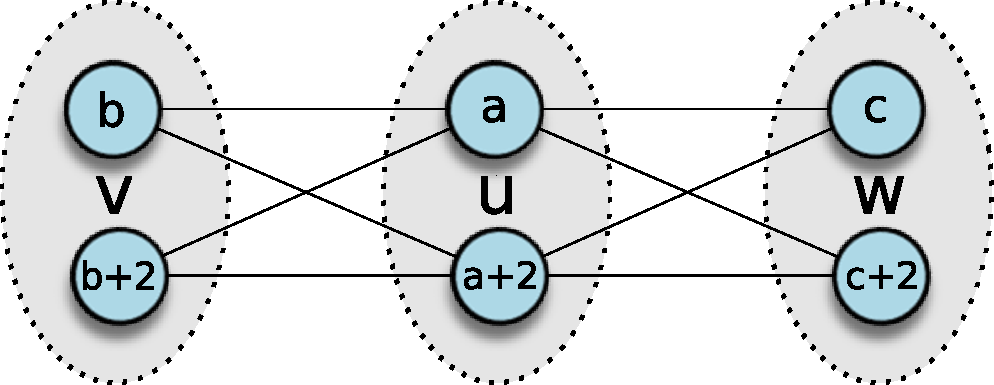
\includegraphics[height=.15\textheight]{pics/zig-zag-neighborhood}
  \caption{The neighborhood of $(u,a)$ in $K_5 \protect\zigzag C_4$.\label{fig:zz_nhbd}}
  \end{minipage}
\end{figure}

The next proposition establishes the connection between adjacency in $K_5 \zigzag C_4$ and parity in $K_5$. More specifically, for each chain of adjacent vertices $\left(w, c\right) \sim \left(u, a \right) \sim \left(v,b\right)$, the vertices $v$ and $w$ will have the same $u$-parity. 
 
 \begin{proposition}
 \label{prop:parity}
 With the same notation as Proposition~\ref{prop:zz_nhbd_formula},  $\enum_u(v) =  \enum_{u}(w) \bmod{2}$.
 \end{proposition}
 \begin{proof}

We have that $\enum_{u}(v) = a + 1 \bmod{4}$ and $\enum_{u}(w) = a -1 \bmod{4}$. Thus $\enum_{u}(v) - \enum_{u}(w) = 2 \bmod{4}$.
\end{proof}

\noindent
And finally we establish that adjacencies are shared amongst the pair of vertices $(u,a)$ and $(u,a+2\bmod{4})$. 

\begin{proposition}
\label{prop:slice}
$N_{\left(u,a \right)} = N_{\left(u,b\right)}$ if an only if either $a = b$ or $b = a + 2 \bmod{4}$. 
\end{proposition}
\begin{proof}

The case where $a=b$ is trivial, so suppose that $b = a +2\bmod{4}$. Then $b - 1 = a + 1 \bmod{4}$ and $b -1 = a + 1 \bmod{4}$. Thus by Proposition~\ref{prop:zz_nhbd_formula} we have that $N_{(u,a)} = N_{(u,b)}$. 

Now for the converse, suppose that $N_{\left(u,a \right)} = N_{\left(u,b\right)}$. For $\left(w,c\right) \in N_{\left(u,a\right)}$ we have that $(w,c) \sim (u,a)$ and $(w,c) \sim (u,b)$, which implies that \[ w = \enum_{u}^{-1}\left(a \pm 1 \bmod{4} \right) = \enum_{u}^{-1}(b \pm 1 \bmod{4}).\] Since $\enum_{u}$ is a bijection, this implies that $ a \pm 1 = b \pm 1 \bmod{4}$. Thus either $a=b$ or $a \neq b$ and $a = b + 2 \bmod{4}$.
\end{proof}

Recall from Section~\ref{sec:class-parity-circ}, that for an enumeration $\Enum$, $\left[u_1\ u_2\  \cdots u_k\right]$ is a parity circuit if for each triple $u_{i-1}$, $u_{i}$ and $u_{i+1}$, $u_{i-1}$ and $u_{i+1}$ have the same $u_{i}$-parity for all $i$ modulo $k$. However we just discarded this information once the parity circuit had been constructed. With that in mind, let $\left[u_1\ \cdots\ u_k\right]$ be a parity circuit of $K_5$ with enumeration $\Enum$. We will say that this circuit has parity $a_i \in \left\{0,1 \right\}$ at $u_i$ for each $i$ where \[ a_i = \enum_{u_i}(u_{i+1}) \bmod{2}.    \] With this additional information we are ready to present a theorem which demonstrates that there is a one-to-one correspondence between every parity circuit of $K_5$ with every $2$-trellis in $K_5 \zigzag C_4$. 

\begin{theorem}
\label{thm:zzcorrespondence}
$\left[u_1\  \cdots\  u_k\right]$ is a parity circuit with parity $a_i$ at $u_i$ if and only if $K_5 \zigzag C_4$ has a subgraph that is a  $2$-trellis over $C_k$ with $S_i = \left\{ (u_i, 1-a_i), (u_i, 3-a_i)\right\}$ for $i =1,\ldots,k$.
\end{theorem}

\begin{proof}

For all $i$, $u_i$, $u_{i+1}$ and $u_{i-1}$ are distinct and $\eta_{u_i}(u_{i-1}) = \eta_{u_i} ( u_{i+1}) = a_i \bmod{2}$ by construction. We would like to say that each element of $S_i$ is adjacent to each element of $S_{i+1}$ in the zig-zag product. From Proposition~\ref{prop:everything}, we just need to check that \[ \left(1-a_i\right) \equiv \eta_{u_i}(u_{i+1}) +1 \bmod{2} \qquad \textrm{and} \qquad \left(1-a_{i+1}\right) \equiv \eta_{u_{i+1}}(u_{i}) +1 \bmod{2}.\] The desired result follows immediately.

Conversely, suppose that the zig-zag product has a subgraph that is a  $2$-trellis over $C_k$ with \[S_i = { (u_i, 1-a_i), (u_i, 3-a_i)}\  \textrm{for}\  i =1,\ldots,k.\] Since elements of $S_i$ are adjacent to elements of $S_{i+1}$ in the zig-zag product, \[\left(1-a_i\right) \equiv \eta_{u_i}(u_{i+1}) +1 \bmod{2}\qquad \textrm{and}\qquad \left(1-a_{i+1}\right) \equiv \eta_{u_{i+1}}(u_{i}) +1 \bmod{2}.\] Then $a_i \equiv \eta_{u_i} (u_{i+1}) \bmod{2}$ and $a_{i+1} \equiv \eta_{u_{i+1}}(u_i) \bmod{2}$. Thus by shifting indices on the last equation, $a_{i} \equiv \eta_{u_{i}}(u_{i-1}) \bmod{2}$. So $\eta_{u_i}(u_{i+1}) \equiv  \eta_{u_i} (u_{i-1}) \bmod{2}$.
This shows $\left[u_1\ \cdots\  u_k\right]$ is a parity path in $K_5$
\end{proof}

With the correspondence between parity circuits and trellis subgraphs establish, we would like to show that these form a complete list of connected components of the zig-zag product. 
\begin{theorem}
\label{thm:final_theorem}
Each connected component of $K_5 \zigzag C_4$ is a $2$-trellis over a cycle $C_j$.
\end{theorem}

\begin{proof}

Let $\Enum$ be an enumeration of $K_5$. Then by Theorem~\ref{thm:unique_pcd} there exists a unique parity circuit decomposition $\pcd = \left( \ppath_1, \ldots, \ppath_m \right)$ which has signature $k_1,\ldots,k_m$. By \ref{thm:zzcorrespondence} there exists a sequence of disjoint subgraphs $\left\{ \trellis_{\ppath_1},\ldots, \trellis_{\ppath_m}\right\}$ where for each $i$,  $\trellis_{\ppath_i}$ is a $2$-trellis over $C_{k_i}$. It is fairly clear that each $2$-trellis is a connected component of $K_5 \zigzag C_4$.

 Conversely, we would like to show that this list is complete. By definition, each graph $\trellis_{\ppath_i}$ has $2k_i$ vertices. Since each is disjoint by construction, by Theorem~\ref{thm:K_5partition10} there exactly \[ 2k_1 + 2k_2 +\cdots+ 2k_m = 2(k_1 + \cdots + k_m) = 2 \cdot 10 = 20\] vertices in this collection of trellis graphs. Since there is a total of $20$ vertices in $K_5 \zigzag C_4$ all vertices have been exhausted and there are no other connected components of $K_5 \zigzag C_4$. 
\end{proof}

Therefore, since each connected component of $K_5 \zigzag C_4$ is a $2$-trellis associated with a unique parity circuit where the defining property is the length of the circuit, we have that the composition of the $2$-trellises is governed solely by the signature of the PCD. Thus by Theorem~\ref{thm:K_5partition10} we have the following theorem: 

\newpage
\begin{theorem}
  \label{thm:zigzag_cats}
$K_5 \zigzag C_4$ is equal to, modulo graph isomorphism,  either
\begin{itemize}
\item $\trellis_3 \sqcup \trellis_3 \sqcup \trellis_4$,
\item $\trellis_3 \sqcup \trellis_7$,
\item $\trellis_4 \sqcup \trellis_6$,
\item $\trellis_5 \sqcup \trellis_5$, or
\item $\trellis_{10}$.
\end{itemize}

\noindent
where $\trellis_n$ is a $2$-trellis on $2\cdot n$ vertices. All of which are depicted in Figure~\ref{fig:zzclass}. 
\end{theorem}

\begin{figure}[H]
\centering
\begin{minipage}{.88\textwidth}
$
\begin{array}[h]{ccc}
  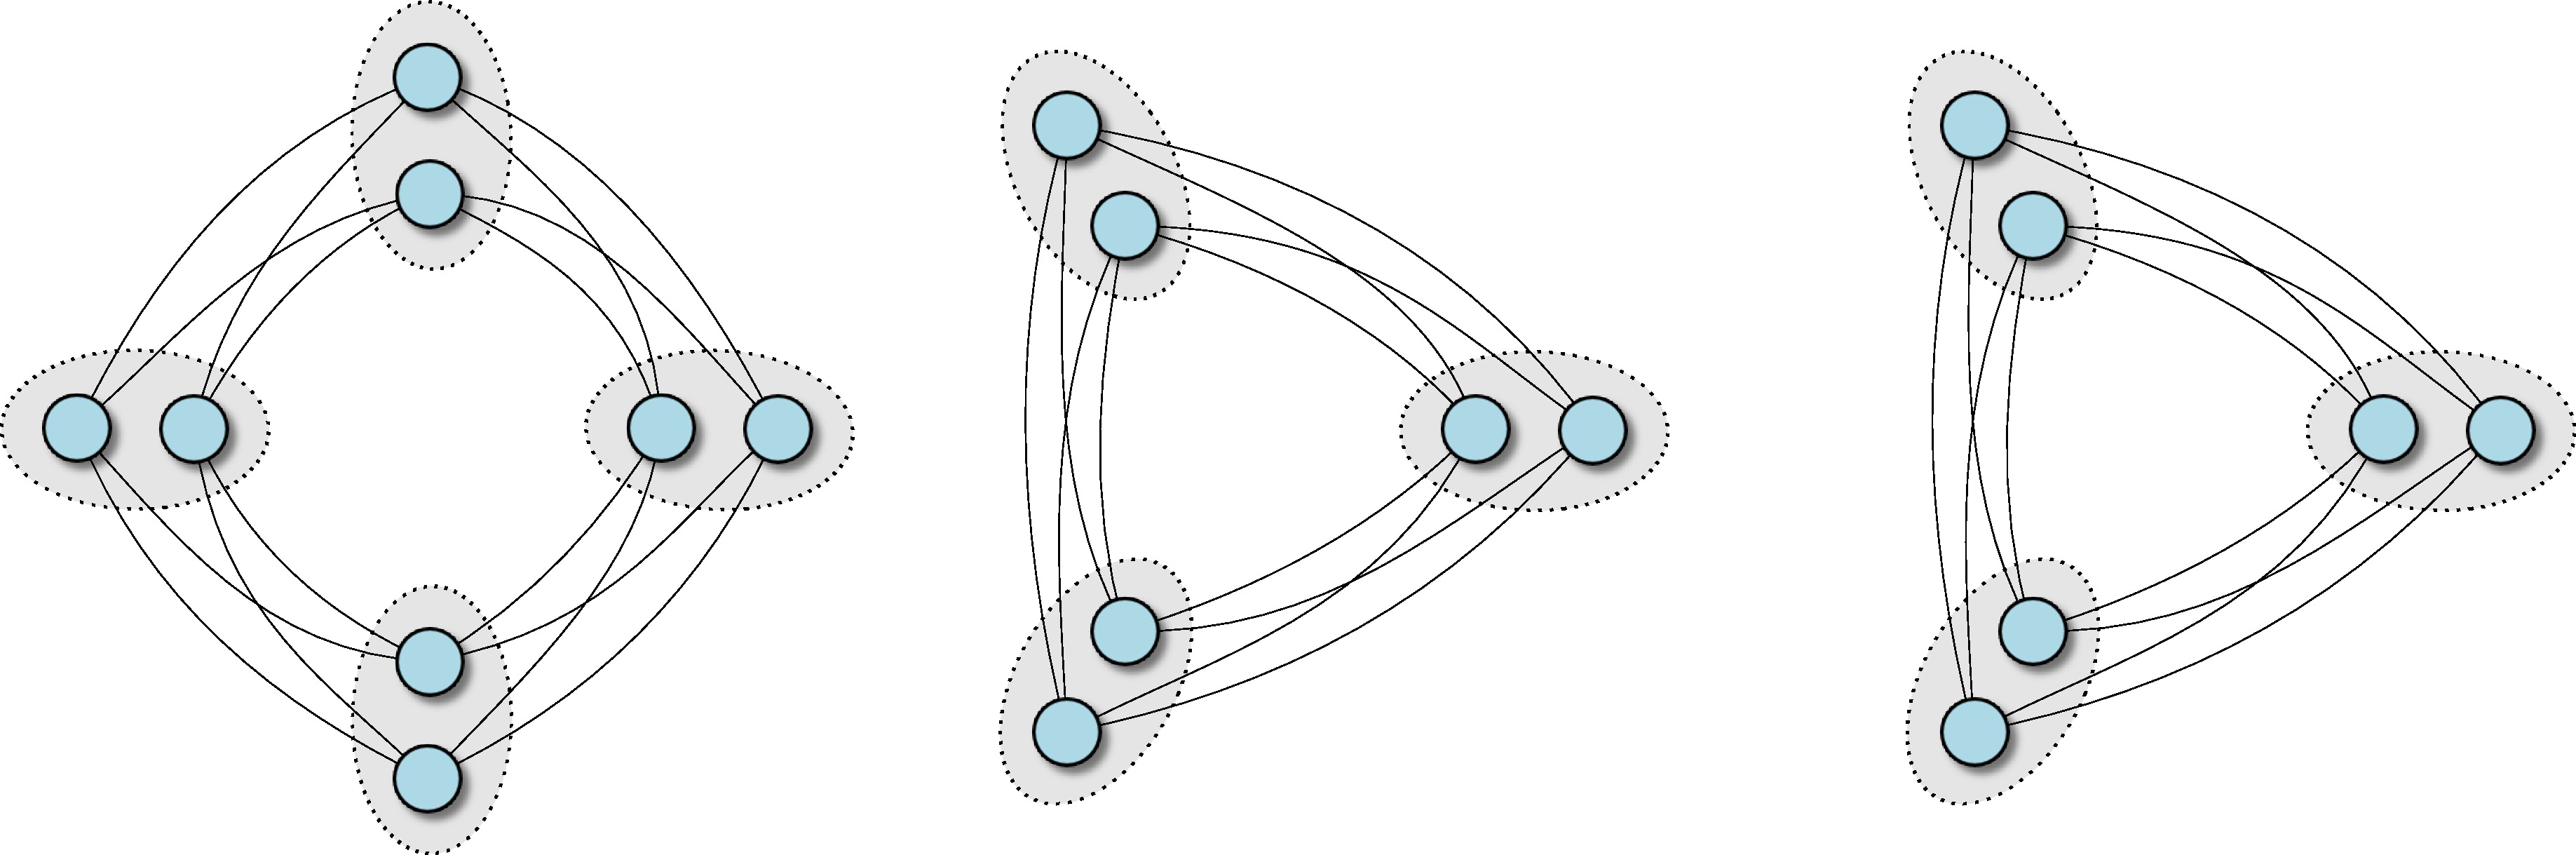
\includegraphics[width=.38\textwidth]{pics/3-3-4-zigzag}\label{fig:334zz} &
  &
  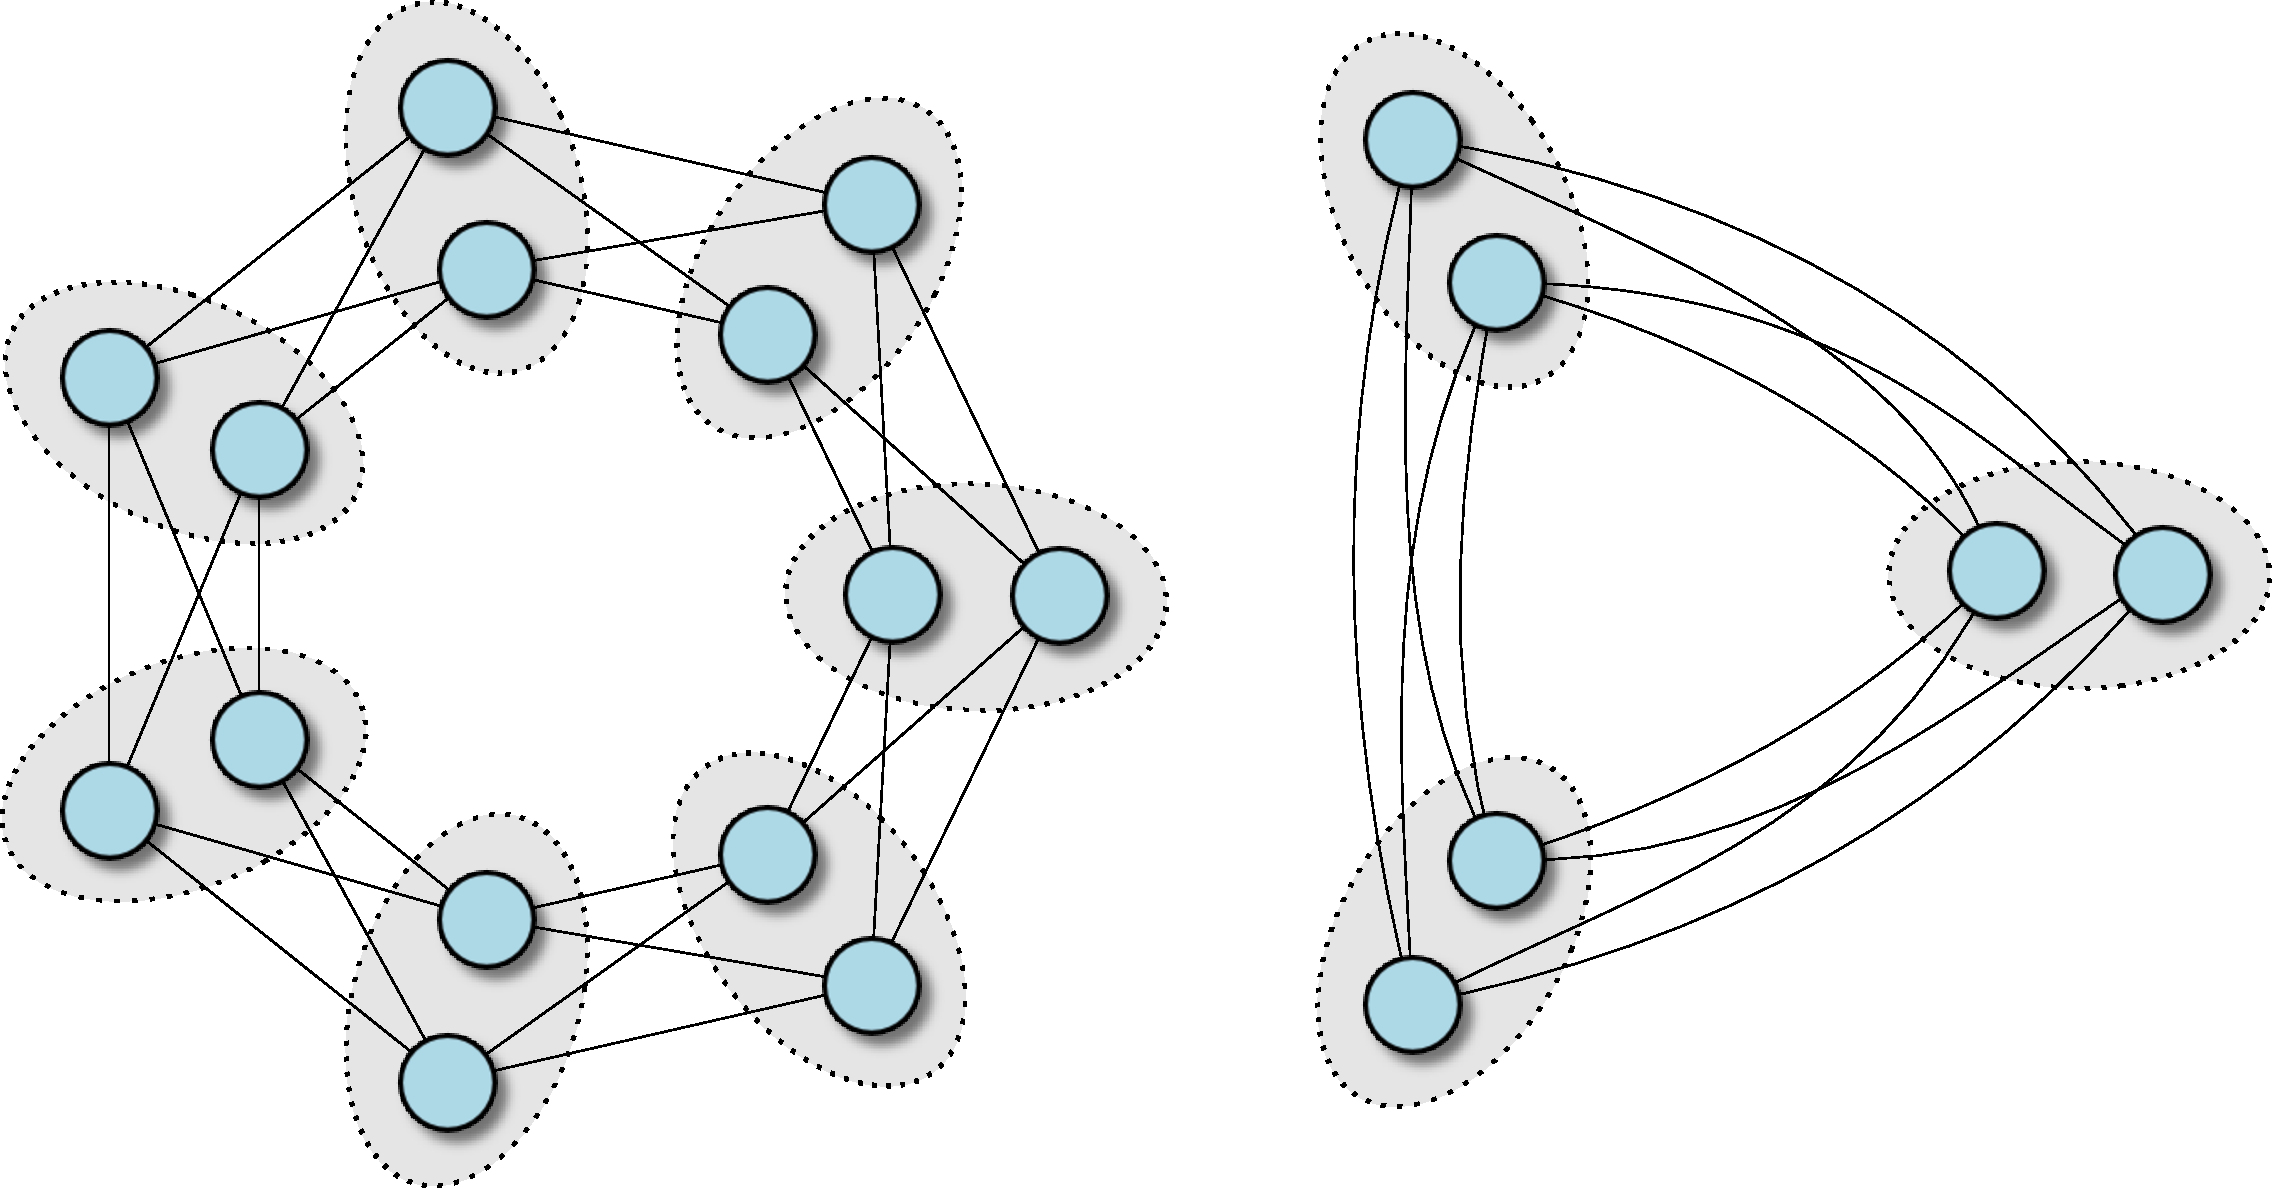
\includegraphics[width=.38\textwidth]{pics/3-7-zigzag}\label{fig:37zz} \\
  \vspace{.05\textheight}\\
  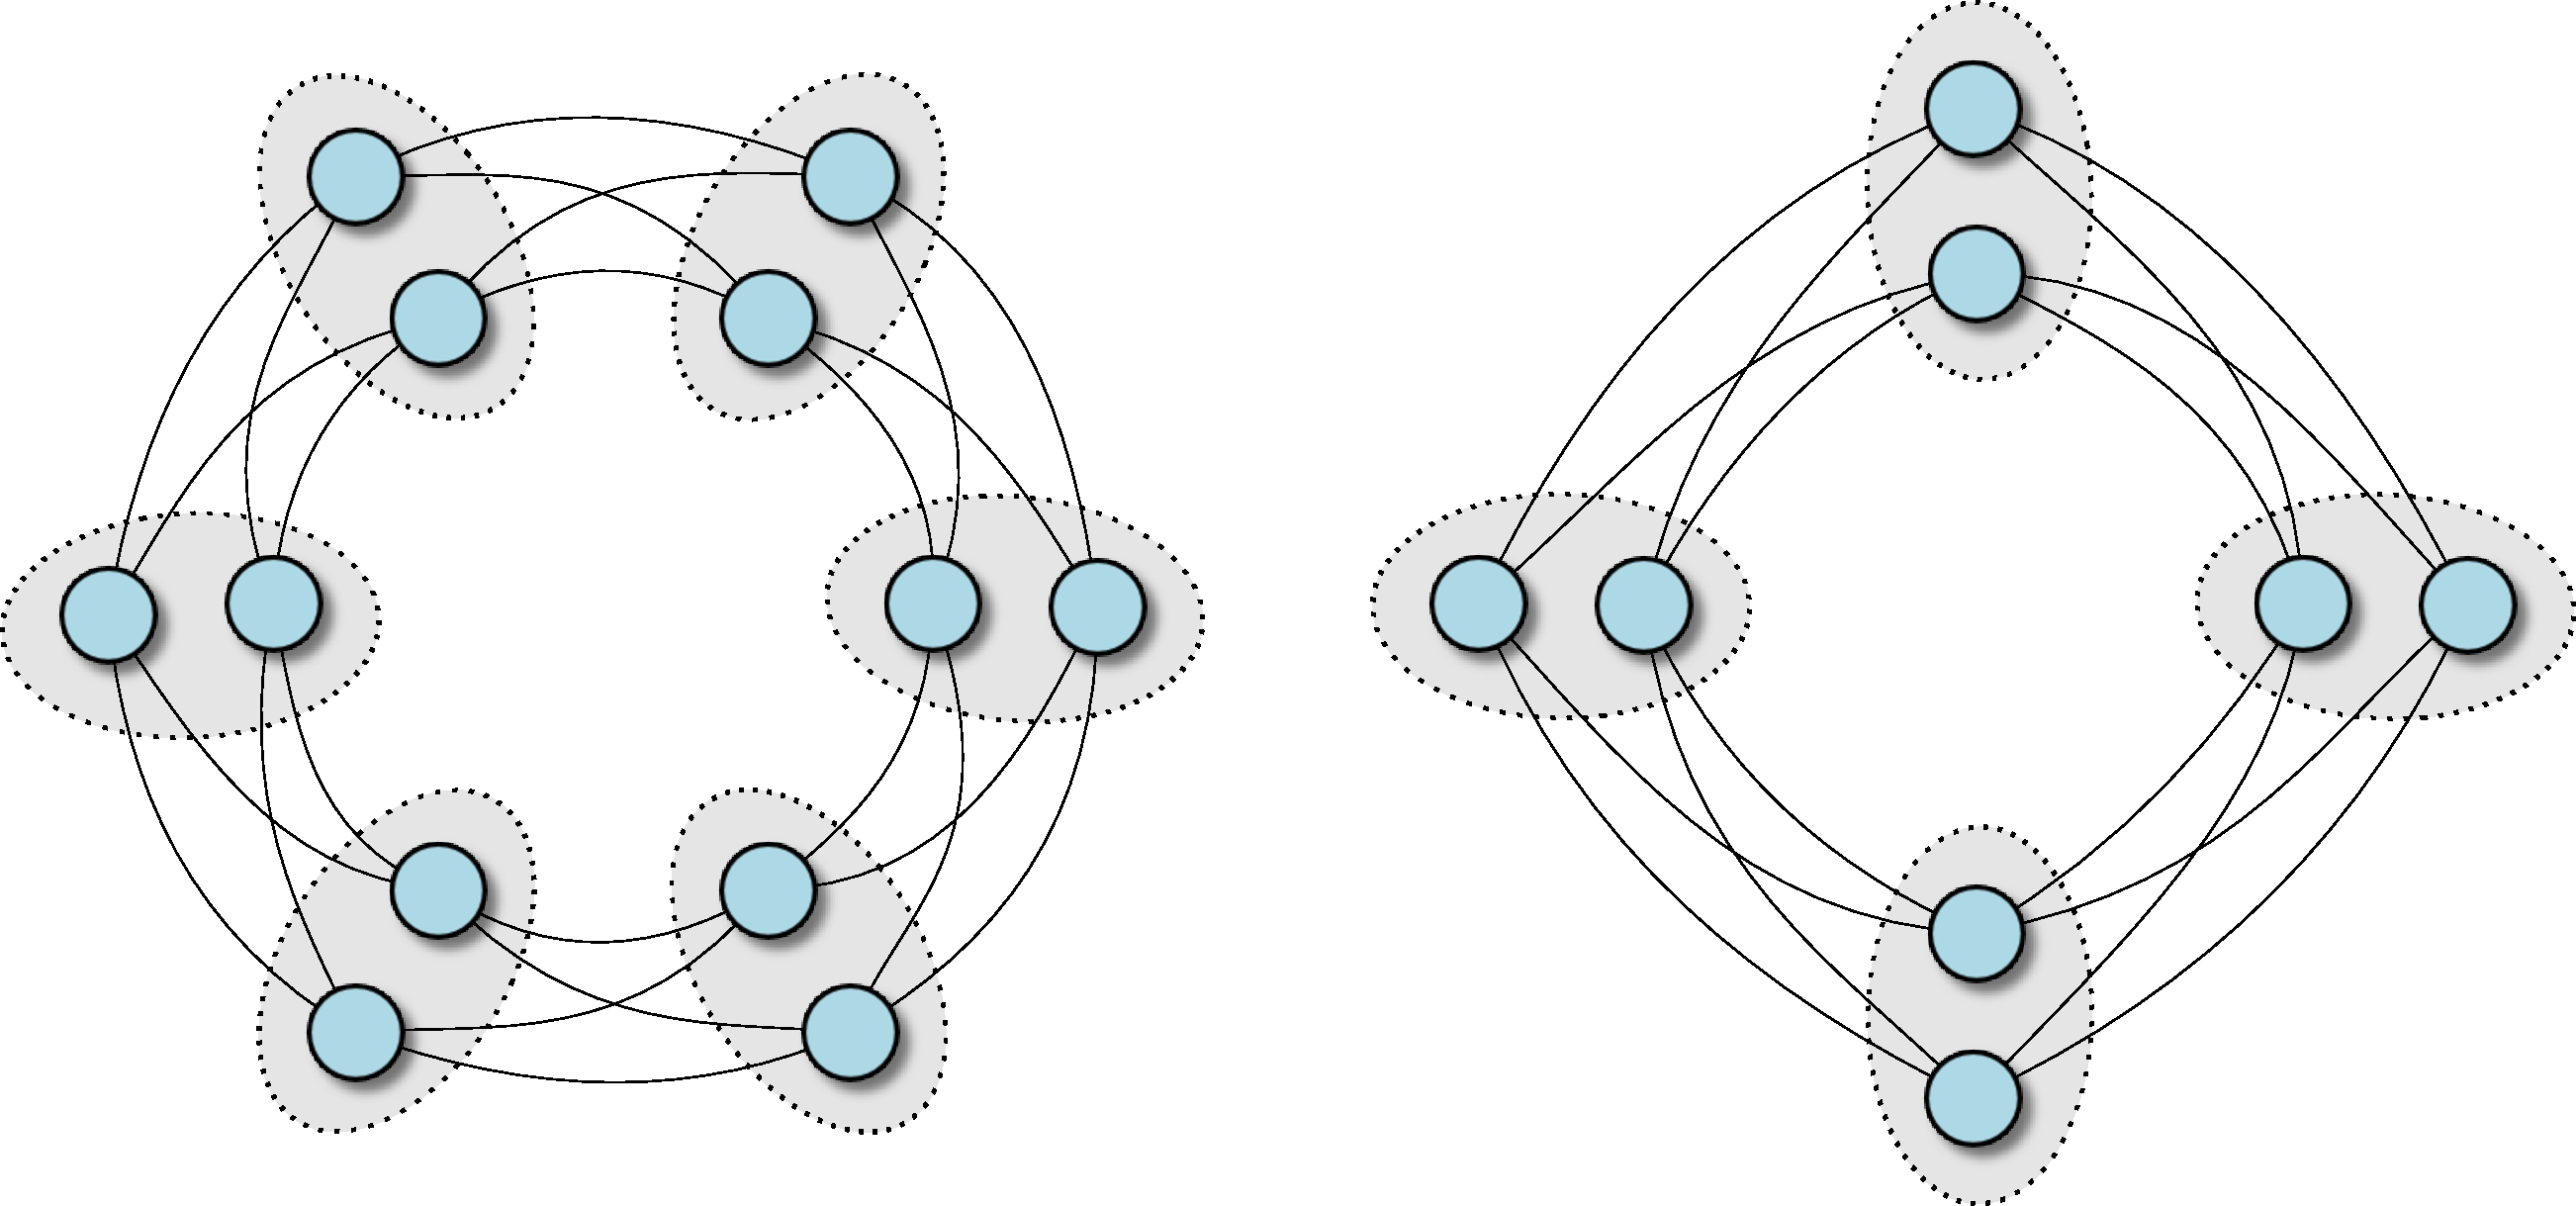
\includegraphics[width=.38\textwidth]{pics/4-6-zigzag}\label{fig:46zz} &
  &
  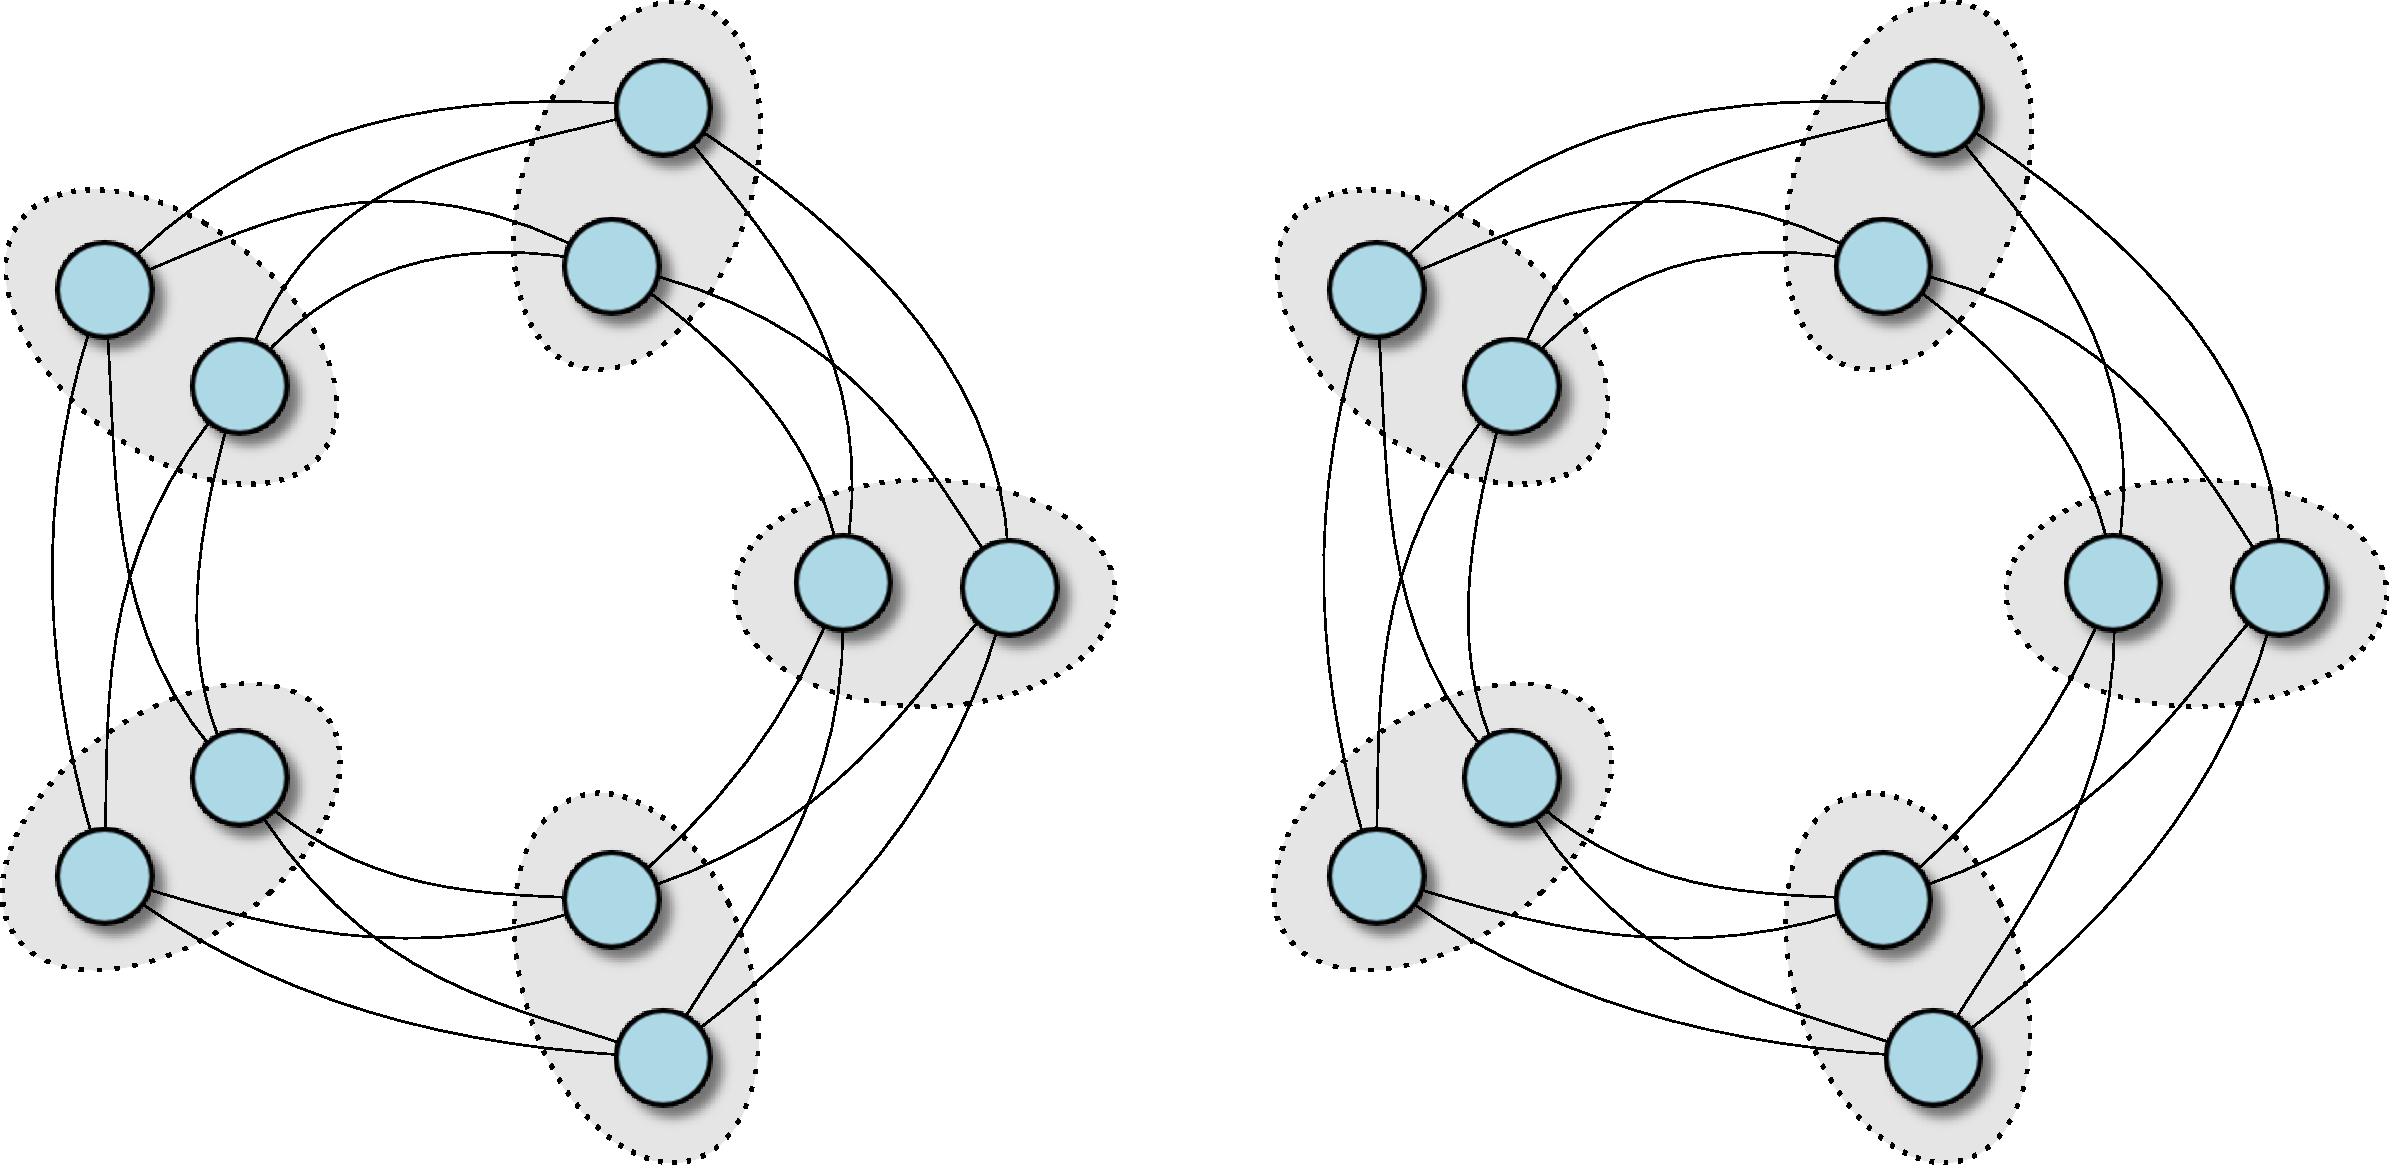
\includegraphics[width=.38\textwidth]{pics/5-5-zigzag}\label{fig:55zz} \\
  \vspace{.05\textheight} \\
  &
  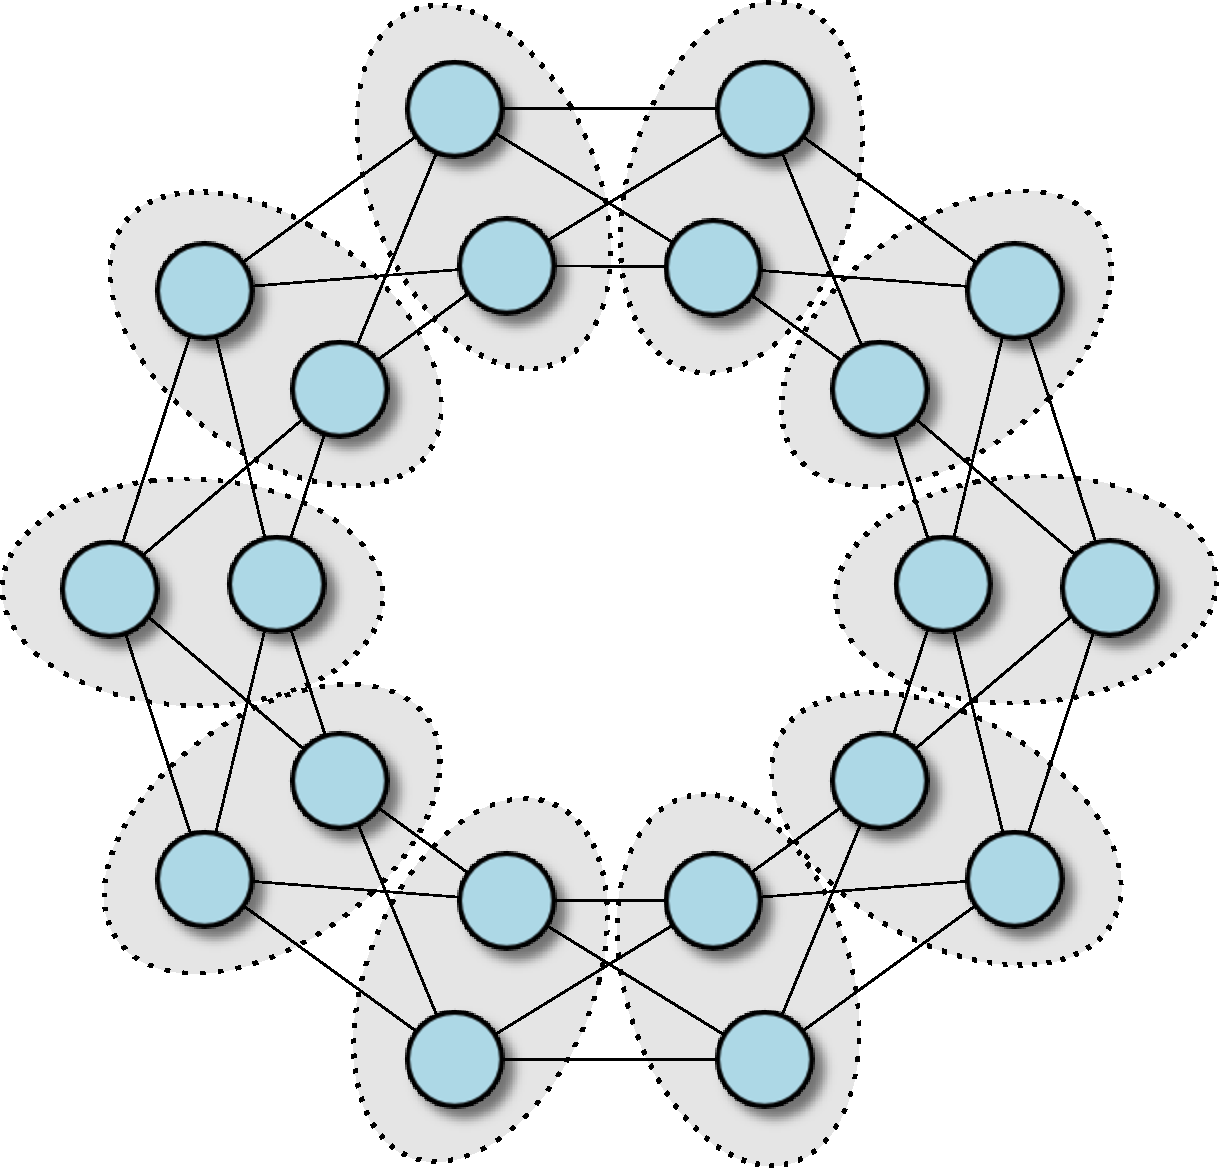
\includegraphics[width=.24\textwidth]{pics/10-zigzag}\label{fig:10zz} &
\end{array}
$
\caption{The $5$ isomorphism classes of $K_5 \protect\zigzag C_4$.\label{fig:zzclass}}
\end{minipage}
\end{figure}

% It should be noted that even though the three types of PCD with signature $10$ were not equivalent under the action provided by $S_5$, the structure of a $2$-trellis is so rigid that the images are still isomorphic.

\chapter{Further topics and generalizations}
\label{chapt:new}

In this section we will break down the zig-zag product into constituents that are simple and relatively easy to understand. Our approach does not require the regularity of the first graph to be equal to the number of edges in the second graph, moreover, neither graph needs to be regular. We use  definitions of digraph and of graph that  allow for loops and parallel edges. The definition is perhaps not standard but can be found in Harary~\cite{Harary:1966} (where the term {\it net} is used instead of digraph) and is close to definitions used by {Mac Lane}~\cite{Lane:1971ys}, and Serre~\cite{Serre:1980}.We  introduce the {\em concatenation} and the {\em sandwich product} of graphs and we demonstrated that the zig-zag product of graphs may be concisely presented as the sandwich product of two relatively simple graphs.

\section{Directed and Undirected Graphs} 
\label{sec:direct-undir-graphs}
In the following definitions, a graph is a digraph with additional structure.

\begin{definition}
\label{def:digraph}
A {\bf directed graph} (or {\bf digraph}), denoted by the letter $G$, is a collection of two sets $\edgeG$ and $\vertG$ together with two functions $\Source_G$ and $\Term_G$ from $\edgeG$ to $\vertG$ where  
\begin{itemize}
\item $\edgeG$ and $\vertG$ are known as the {\bf edge} and {\bf vertex} sets of the digraph $G$.
\item $\Source_G$ and $\Term_G$ are known as the {\bf source} and {\bf terminus} functions of the digraph $G$.
\end{itemize}
\end{definition}

\begin{definition} 
An \textbf{undirected graph}, or just \textbf{graph},  is a digraph $G$ in which there exists a unique involution $\Rot_{G}:E \mapsto E$ such that $\Term_G = \sigma_G \circ \Rot_G$. We call the function $\Rot_G$ the {\bf rotation mapping} of the graph $G$.
\end{definition}

The term rotation map was first used in Reingold {et al.}~\cite{Reingold:2002ys} though our definition is more general than that which was provided. In the usual depiction of a graph an edge between two vertices represents two edges according to  the preceding definition: one going each direction, and  the two are images of each other under the rotation map $\Rot_G$. Also we consider two vertices $u, v \in \vertG$ as {\em adjacent} in $G$ if there exists and $e \in \edgeS{G}$ such that $\source{e} = u$ and $\source{\Rot\left(e \right)} = v$.

We will often depict the sets and mappings of our digraphs and graphs with the use of the diagrams
\[
\xymatrix{ \edgeS{G} \ar@<-.5ex>[d]_{\Source_G} \ar@<+.5ex>[d]^{\Term_G} \\ \vertS{G} } \quad \quad \xymatrix{ \edgeS{G} \ar@(ul,ur)^{\Rot_G} \ar[d]^{\Source_G} \\ \vertS{G} }
\]
respectively.

If we have two graphs $G$ and $H$ we will say that they are equal, or equivalent if there exists a pair of bijections $f:\edgeS{G} \longleftrightarrow \edgeS{H}$ and $g:\edgeS{G} \longleftrightarrow \edgeS{H}$ such that the following diagrams commute.
\[
\xymatrix{ \edgeS{G}  \ar[d]_{\Source_G} \ar@{<->}[r]^{f} & \edgeS{H}  \ar[d]^{\Source_H}  \\  \vertS{G} \ar@{<->}[r]^{g} & \vertS{H} } \hspace{.10\textwidth}
\xymatrix{ \edgeS{G}  \ar[d]_{\Rot_G} \ar@{<->}[r]^{f} & \edgeS{H}  \ar[d]^{\Rot_H}  \\  \edgeS{G} \ar@{<->}[r]^{g} & \edgeS{H} }
\]
Essentially all $f$ and $g$ are is edge and vertex re-labellings which preserve adjacency.  

The tip to tail concatenation of the graphs used in the definitions of the zig-zag and replacement products has a connection to a more general construct, the {\em pullback} of mappings of sets, that is defined as follows:

\begin{definition}
\label{definition:pullback:set}
Let $A$, $B$, and $C$ be sets and let $f:A \mapsto C$ and $g:B \mapsto C$ be functions. Then the {\bf pullback} of set  functions $f$ and $g$ is the set \[ A \times_{C} B = \left\{  \left( a, b \right) \in A \times B\  \vert\  f\left(a\right) = g\left(b\right) \right\}  \] together with the standard coordinate projections $\pi_{1}$ and $\pi_{2}$.
\end{definition}

We can look at the tip to tail traversing of the edges of two graphs in the zig-zag product as really just the pullback of the terminus of one graph with the others source mapping. The digraph that we get when we make adjacent the verticies at the endpoints of this traversal we call the {\em concatenation}, which is defined as follows:
\begin{definition}
Let $G$ and $H$ be directed graphs with a common vertex set $V$ and let $E(G) \times_{V} E(H)$ be the pullback of the mappings $\Term_{G}$ and $\Source_{H}$.  Then the \textbf{concatenation} of $G$ with $H$, denoted by $G \concat H$,  is the directed graph with vertex set $V$,
edge set $E(G) {\times_{V}} E(H)$ , source map $\Source = \Source_{G} \circ \pi_{1}$ and terminus map $\Term = \Term_{H} \circ \pi_2$ as depicted in the diagram 
\[
\xymatrix{
   & E(G) \times_{V} E(H) \ar@<-.25em>[dd]_{\Source} \ar@<+.25em>[dd]^{\Term} \ar[dr]^{\pi_2} \ar[dl]_{\pi_1} &  \\
 E(G) \ar[dr]_{\Source_G}  & &  E(H) \ar[dl]^{\Term_{H}}  \\
   & V & 
}
\]
\end{definition}

Note that the concatenation of two undirected graphs is not necessarily a graph, as can be seen in Figure~\ref{figure:example:concatenation}, which depicts a $3$-cycle. There are $6$ edges, $a,b,c,d,e,f$ each of which is labeled next to it's source. Edge $1$ has source $1$ and terminus $0$; it's rotation image is $b$, which has source $0$ and terminus $1$. 

\begin{figure}[h!]
\centering
\begin{minipage}{.85\textwidth}
$
\begin{array}[h]{ccc}
  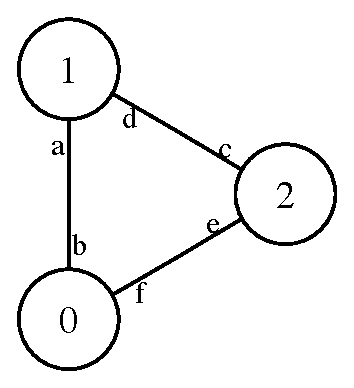
\includegraphics[scale=.50]{three_cycle} & 
  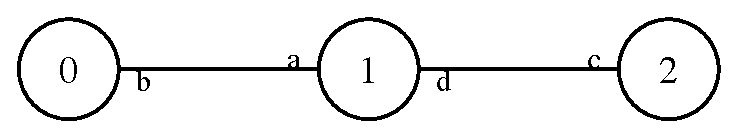
\includegraphics[scale=.50]{line} & 
  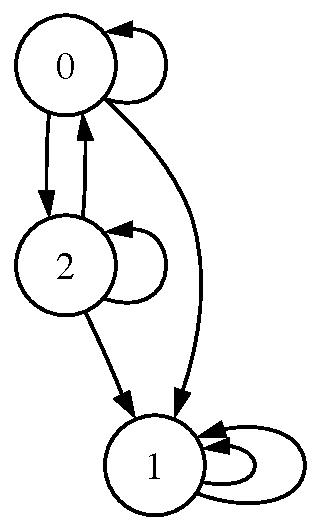
\includegraphics[scale=.50]{concatination}
\end{array}
$
\caption{Three-cycle, three-chain (with indicated source and terminus labeling) and their concatenation.\label{figure:example:concatenation}}
\end{minipage}
\end{figure}

While  $G \concat H$ is not guaranteed to be a graph, the double concatenation of the form $G \circ H \circ G$ always is. We will call this type of concatenation  the {\em sandwich product}, an example of which is illustrated in Figure~\ref{fig:sandwich}.

\begin{definition}
Let $G$ and $H$ be graphs with common vertex set $V$. Then the {\bf sandwich product} of $G$ with $H$, denoted $G \sandwich H$, is the graph with vertex set $V$, edge set 
\[
\edgeS{G \sandwich H} = \left\{ ( f,e,f^{\prime} ) \in \edgeS{H} \times \edgeS{G} \times \edgeS{H}  \ \vert \ \Term_{H}\left(f \right) = \Source_{G}\left(e \right)  \ {\rm and} \ \Term_{G}\left(e \right) = \Source_{H}\left(f^{\prime} \right) \right\}
\] with source map which takes $(e,f,e^{\prime}) \mapsto (\Source_{G}(e) , \Source_{H}(f))$ and rotation map \[\Rot((f,e,f^{\prime})) = \left(\Rot_{H}(f) , \Rot_{G}(e) ,\Rot_{H}(f^{\prime})\right)\]  
\end{definition}

\begin{figure}[h!]
\centering
\begin{minipage}{.85\textwidth}
\[
\begin{array}{ccc}
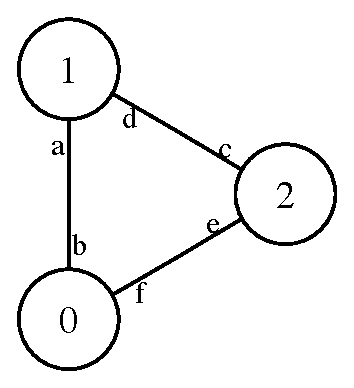
\includegraphics[scale=.50]{three_cycle} &  
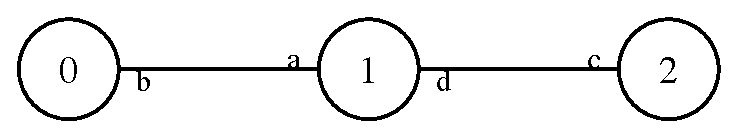
\includegraphics[scale=.50]{line} & 
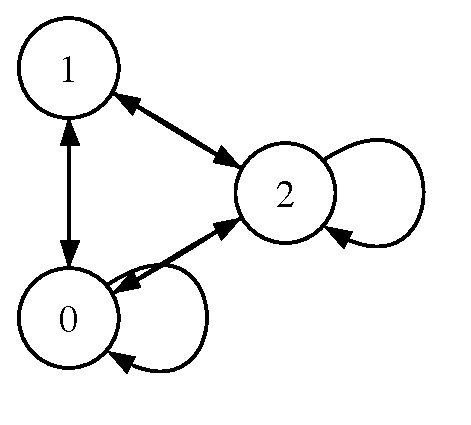
\includegraphics[scale=.50]{sandwich} 
\end{array}
\]
\caption{The Sandwich Product of a three cycle and a three chain (with indicated source and terminus labeling). \label{fig:sandwich}}
\end{minipage}
\end{figure}

The sandwich product is a ``zig-zag'' like product but with little more required of $G$ and $H$ than they have the same vertex set. It is still left to be shown what properties, expansion or otherwise, that this products has. 


\section{A Zig-Zag Sandwich}
\label{sec:zig-zag-sandwich}
We now can display the zig-zag product of two graphs as the sandwich product of two simple graphs. 
The first factor we call the zig product and the second factor the zag product.  

\begin{definition}
\label{def:graph:zig} 
Let $G$ and $H$ be graphs. The the \textbf{zig product} of $G$ with $H$, denoted $G \zig H$,  is the graph depicted in the diagram
\[ 
\xymatrix{
  {V(G) \times E(H)} \ar[d]_{id_{V(G)} \times \Source_{H}}  \ar@(ul,ur)^{id_{V(G)} \times \Rot_{H}}  \\
     {V(G) \times V(H)}
}
\]
\end{definition}
The zig product graph will lie at the beginning and end of our product much like how we start and end in a ``cloud'' when we traverse the replacement product graph in a ``zig-zag'' fashion. In fact the graph is exactly just $\card{\vertS{G}}$ disjoint copies of $H$. We now need to define our analog to the bridges between the ``clouds'' in the zig-zag. We will call this graph the {\em zag product}
\begin{definition} 
\label{def:symnet:zag}
Let $G$ and $H$ be graphs and let $\phi:\edgeS{G} \mapsto \vertS{H}$ be an onto mapping. The {\bf zag product} of $G$ and $H$, denoted $G \zag H$, is the graph with  vertex set $V(G) \times V(H)$, 
edge set $\edgeS{G \zag H} = \edgeS{G}$, source mapping $\Source_{\rm zag} = \Source_{g} \times \phi$ and rotation mapping $\Rot_{\rm zag} = \Rot_{G}$ as depicted the diagram 
\[
\xymatrix{
  {E(G)} \ar[d]_{\Source_{G} \times \phi} \ar@(ul,ur)^{\Rot_{G}}  \\
  V(G) \times V(H)
}
\]
\end{definition}

The definition above requires only a mapping from the edges set of $G$ to the vertex set of $H$. It is more general then the one in the paper by Reingold {et al.}~\cite{Reingold:2002ys} in which $G$ must be regular of degree equal to the number of vertices in $H$.

We are now ready to define the {\em zig-zag} product using the language developed in this section.

 \begin{definition}
 \label{def:cat_zigzag}
Let $G$ and $H$ be graphs with $\phi:\edgeS{G} \mapsto \vertS{H}$. Then the {\bf zig-zag} product of $G$ with $H$, denoted $G \zigzag H$, is the graph with vertex set $V(G) \times V(H)$,  edge set
\[ E(G \zigzag H) = \left\{  \left( f, e, f^{\prime} \right) \ \vert \ \Term_H\left(f\right) = \phi\left(e\right)\ \textrm{and} \  \phi\left( \Rot\left(e \right)  \right) = \Source_{H}\left(f^{\prime}\right)  \right\}, \] source mapping given by $\Source\left( \left(f, e, f^{\prime}\right)\right) = \left( \Source_G \left(e \right), \Source_{H}\left( f \right) \right)$ and rotation mapping $\Rot$ given by  \[ \Rot(e,f,e^{\prime}) = \left( \Rot_{H}\left( f^{\prime} \right) , \Rot_{G} \left( e \right), \Rot_{H } \left( f \right) \right)  \]
\end{definition}

Next we will present a small theorem that connects the zig-zag to the sandwich product. 
\begin{theorem}
\[ G \zigzag H = \left( G \zag H \right) \sandwich \left( G \zig H \right)
                   \]
\label{thm:zigzagsandwich} 
\end{theorem}

\begin{proof}

Let $f: \edgeS{ \left( G \zag H\right) \sandwich \left(G \zig H \right) } \mapsto \edgeS{G \zigzag H}$ be the mapping that sends the edge $\left(\left(v,f\right), e, \left(v^{\prime}, f^{\prime}\right)\right)$ to the edge $\left(f, e, f^{\prime} \right)$ and let $g$ be the identity mapping from $\vertS{G} \times \vertS{H}$ to itself. First we will show that the source is preserved through this mapping. Let $\Source_s$, $\Rot_s$ be the source and rotation mappings for the sandwich product and let $\Source_z$, $\Rot_z$ be the source and rotation mappings for the zig-zag product. We have that \[ 
\Source_{s}\left( ((v,f),e,(v^{\prime},f^{\prime} )) \right) =   (v, \Source_H\left(f\right) )
\] and \[ 
\Source_{z}\left((f,e,f^{\prime})\right) = \left(\Source_{G}(e), \Source_{H}(f) \right)
\] Since $((v,f),e,(v^{\prime},f^{\prime} )$ is an edge in $ \left( G \zig H\right) \sandwich \left(G \zag H \right)$ we have that \[ (v, (\Source_H \circ \Rot)(f))  = (\Source_{G}(e), \phi(e)   ) \qquad \textrm{and} \qquad (  (\Source_G \circ \Rot)(e), (\phi \circ \Rot)(e)) = ( v^{\prime}, \Source_{H}(f^{\prime}))   \] which implies that $\Source_{G}(e) = v$. Therefore we can conclude that images under their source mappings are identical. Now consider the terminus mapping $\Term = \Source \circ \Rot$ \[
 (\Source_s \circ \Rot_s)((v,f),e,(v^{\prime},f^{\prime} )) = (v^{\prime}, (\Source_H \circ \Rot_h)(f^{\prime}))  
\] and \[
 (\Source_z \circ \Rot_z)(f,e,f^{\prime}) = ( (\Source_G \circ \Rot_G)(e), (\Source_H \circ \Rot_h)(f^{\prime} )) 
\] Which since $(\Source_G \circ \Rot_G)(e) = v^{\prime}$ implies that the terminus is also preserved. Moreover since both $v$ and $v^{\prime}$ are uniquely determined by $e$ we have that the mapping $f$ is a bijection. Thus since $f$ and $g$ are bijections which preserve the graphs source and terminus mappings we have that th two graphs must be equivalent per the criteria previously discussed. 
\end{proof}

The final theorem of this section will show that our old definition of the zig-zag product is a special case of the one presented in this section. To prevent confusion, just for this theorem we will call the more general graph object defined in this chapter a {\em net}, a term borrowed from Harary~\cite{Harary:1966},  whereas we will use the more tradition definition when we use the term graph.

\begin{theorem}
\label{thm:old_new}
Let $G$ be a $d$-regular graph on $n$ vertices and $H$ be a $m$-regular graph on $d$ vertices. Also let $\Enum$ be an enumeration of $G$ with respect to $H$ per the definition provided in Chapter~\ref{chapt:old_zz}. Also define a net $\mathcal{G}$ with edge set $\edgeS{G}$, vertex set $\vertS{G}$, source mapping $\Source\left( \left(u,v\right)\right) = u$ and rotation mapping $\Rot\left(\left(u,v\right)\right) = \left(v,u\right)$. Define $\mathcal{H}$ similarly for $H$. And consider $\phi:\edgeS{\mathcal{G}} \mapsto \vertS{\mathcal{H}}$ given by $\phi\left((u,v)\right) = \enum_u\left(v\right)$. Then for each $\left(u,a\right), \left(v,b\right) \in \vertS{G} \times \vertS{H}$, $(u,a)$ is adjacent to $(v,b)$ in $\mathcal{G} \zigzag \mathcal{H}$ if an only if $\left(u,a\right)$ is adjacent to $(v,b)$ in $G \zigzag H$ (per Definition~\ref{def:zig_zag:old}).  
\end{theorem}

\begin{proof}
Suppose that $\left(u, a\right)$ is adjacent to $\left(v, b \right)$ in $\mathcal{G} \zigzag \mathcal{H}$ This means that there exists $e \in \edgeS{G}$ and $f,f^{\prime} \in \edgeS{H}$ such that $\Source_G(e) = u$, $\Source_{H}(f) = a$, $(\Source_H \circ \Rot_H)(f^{\prime}) = b$ and $(\Source_G \circ \Rot_G)(e) = v$. So let $c = \phi(e) = \enum_u(v) $ and $d = (\phi \circ \Rot)(e) = \enum_v(u)$. Then since $\left(a, \phi(e)\right)$ and $\left((\phi \circ \Rot)(e)), b\right)$ are in  $\edgeS{H}$ we can conclude that $\left(u, a\right)$ is adjacent to $\left(v, b\right)$ in $G\zigzag H$.

For the converse implication let $\left(u, a\right)$ is adjacent to $\left(v, b\right)$ in $G\zigzag H$. Then we know that there exists $c,d$ such that $\left(a,c\right), \left(d,b\right) \in \edgeS{H}$. and $c = \enum_{u}(v)$ and $d = \enum_{v}(u)$.  Let $e = \left(u,v\right)$, $f = \left(a, c \right)$ and $f^{\prime} = \left(d,b\right)$. Then it can be easily shown that $\left(f, e, f^{\prime}\right)$ is an edge in $\mathcal{G} \zigzag \mathcal{H}$ with source image $\left(u,a \right)$ and terminus image of $\left(v,b\right)$. 
\end{proof}
 
\chapter{Conclusion}

Constructing graphs with good expansion properties is an important problem in
applied mathematics and the creation of the zig-zag product of graphs by Reingold {et al.}~\cite{Reingold:2002ys} in 2000 was an important step toward making the use of expander graphs practical. In this thesis we expand on the fact that there are many zig-zag products, which was not emphasized in the original work, and that it makes sense to look into their classifications. We accomplished this by fully examining the replacement and zig-zag products for the complete graph $K_5$ and the cycle graph $C_4$. Recall that the zig-zag and replacement products are defined by two graphs and a correspondence between the edges of one with the vertices of
the other, which we called the enumeration. By examining this small, but non-trivial, example we were able to highlight the relationship between the enumeration and the automorphism groups of $K_5$ and $C_4$. It is our hope that many of the tools developed in this classification have broader applications to more general cases.
We generalized the definition of graph in a manner inspired by Serre~\cite{Serre:1980} and Harary~\cite{Harary:1966}. By looking at graphs as just a vertex set, an edge set and a pair of mappings we were able to construct an elegant description of the zig-zag product, via the more general sandwich product, in this more general setting. In doing so we remove the regularity required in the original definition.

The original paper \cite{Reingold:2002ys} has assisted both in application and as the starting point for numerous advances in research. We hope that this thesis serves as a new perspective on this important work which others will be able to branch out from and develop more fully. By placing the emphasis on the enumerations and how these give rise to differences in the many
zig-zag and replacement products we feel as if we have drawn attention to a significant gap in the current literature. There are many directions in which the work here can be taken,including the following:

\vspace{2ex}
\noindent
{\bf The classification of $G \replacement C_4$ and $G \zigzag C_4$ for any $4$-regular graph}
\vspace{2ex}

The most obvious next step would be to use the notion of parity to extend the
definitions and theorems in Chapter~\ref{chapt:K5zzC4} when $G$ is any $4$-regular graph and not just the complete graph on $5$ vertices. For notions like parity circuit decomposition little work needs to be done to extend the concepts as they almost depend completely on the properties of $C_4$ . Though much is not known about how $\Aut(G)$ being more general affects the classes of PCDs, it is suspected that when $G$ has a small automorphism group there will likely be many classes of
replacement and zig-zag products.

\vspace{2ex}
\noindent
{\bf The Classification of $G \replacement C_n$ and $G \zigzag C_n$ for a general cycle}
\vspace{2ex}

It can be shown that the zig-zag product when taken over $C_4$ is always a $2$-trellis, which is known to have bad expansion properties. It is suspected that the zig-zag product over larger cycles will yield a richer class of graphs with possibly better expansion properties, while still being simple enough that a full classification is practical.

\vspace{2ex}
\noindent
{\bf The Sandwich Product and the generalization to non-regular graphs}
\vspace{2ex}

By considering a graph just a collection of functions which satisfy certain properties, we have opened up an intriguing and, some would say, elegant method for describing the zig-zag product in a more general setting. As it stands today, the definitions are too broad to be useful for analysis, but by placing additional restrictions on the mappings involved there is
hope for further development.

\vspace{2ex}
\noindent
{\bf The Zig-Zag Product and it’s connection with the semi-direct product of groups} \vspace{2ex}

A paper by Alon {et al.}~\cite{Alon:2001xy} presented an interesting connection between the semi-direct product and the zig-zag product of graphs. That with suitably chosen generating sets, the Cayley graphs of the semi-direct product of two groups can be seen as the zig-zag product of the constituent Cayley graphs. If we let $G = \mathbb{Z}_5$ with Cayley generating set $S_G = \mathbb{Z}_5 \setminus \{0\}$
and $H = \mathbb{Z}_4$ with generating set $S_H = \{\pm1\}$, then we have Cayley graphs which mirror $K_5$ and $C_4$ . Obvious questions are how does the structure of the groups effect the enumeration which would be generated by these Cayley graphs. We are still very early in this process.

So in conclusion, as with most mathematical work, we are left with as many questions as we have answers. The hope of the author is that this thesis will be seen as a good first step.

% \section{THE SEMI-DIRECT PRODUCT OF GROUPS}
% \label{sec:semi-direct-product}

% The semi-direct product is, as the name suggests, a generalization of the more commonly discussed {\em direct product} of groups. Central to this generalization is the notion of how a group ``acts'' on another group. The notion of group action we define as follows, 

% \begin{definition}
%   \label{def:group_action}
% Let $H$ and $N$ be groups. The group $H$ {\bf acts} on $N$ if there exists a homomorphism $\Act: H \mapsto \Aut\left(N\right)$. Where the image of $h$ under $\Act$ is the automorphism denoted by $\Act_h$. Also for each $n \in N$ and $h \in H$ we call the {\bf action} of $h$ on $n$ to be the image of $n$ under the automorphism $\Act_h$. For convenience we denote this image $\acts{h}{n}$. 
% \end{definition}
% \noindent

% \begin{definition}
%   \label{def:semi_directproduct}
% Let $H$ and $N$ be groups where $H$ acts on $N$. Then the {\bf semi-direct product} $N \rtimes_{\Act} H$ is a group with elements that are pairs  $\left( n, h\right) \in N \times H$ with the product defined as \[  \left( n_1 , h_1 \right) \left( n_2, h_2 \right) = \left( n_1\left(\acts{h_1}{n_2}\right) , h_1 h_2 \right) \]
% \end{definition}
% \noindent


% \noindent
% For the reader who is unfamiliar with group actions we provide the following examples that we will use in later constructions.


% \begin{example}
%   \label{ex:ga:trivial}
% Let $H$ and $N$ be any two groups and consider the mapping $\Act: H \mapsto \Aut\left( N \right)$ which sends $h \mapsto \id_N$ for all $h \in H$. This action fixes all elements and is called the {\em trivial} group action. The semi-direct product $N \rtimes H$ with the trivial action is isomorphic to the {\em direct product}, $N \times H$. Since \[ (n_1, h_1)(n_2,h_1) = (n_1 \left(\acts{h_1}{n_2}\right), h_1 h_2) = (n_1 n_2, h_1 h_2 )     \] 
% \end{example}

% \begin{example}
%   \label{ex:ga:cyclic}
% Let $N = \left( \mathbb{Z}_{n}^d, +\right)$ be the additive group of the $d$ dimensional vector space over $\mathbb{Z}_n$  and $H = \mathbb{Z}_d$, the cyclic group of order $d$. Let $c_k:N \mapsto N$ be the coordinate-wise {\em cyclic shift} operator. The mapping $\Act: k \mapsto c_k$ constitutes a group action. The semi-direct product $N \rtimes H$ under this group action with a product (written additively) 
% \[
% \left( (i_1, i_2,\ldots,i_d ),l\right) + \left((j_1,j_2,\ldots,j_d),m\right) = \left((i_1 + j_{1+l},i_2 + j_{2+l},\ldots,i_d + j_{d+l}),l + m\right)
% \] where the subscripts are computed modulo $d$. 
% \end{example}

% \begin{example}
%   \label{ex:ga:exp}
% Let $N$ be an abelian group and let $H = \mathbb{Z}_{2k}$. The mapping that takes $a \mapsto \inv$ for $a$ odd and $a \mapsto \mathrm{id}$ for $a$ even is a group action, which is nontrivial when $N$ has an element of order greater than $2$. 

% If we let $H = \mathbb{Z}_2$ and $N = \mathbb{Z}_4$. Then let us examine the semi direct product in which$\Act$ is the action which sends $0 \mapsto id_N$ and $1 \mapsto \inv$ . The resultant $N \rtimes_{\Act} H$ is a group isomorphic to the {\em dihedral} group $D_{4}$ or the collection of symmetries on a square. To see this let $D_4 = \left<(0\ 1)(2\ 3), (0\ 1\ 2\ 3) \right>$ and map $\left(0,1\right) \mapsto \left(0\ 1\right)\left(2\ 3\right)$ and $\left(1,0\right) \mapsto \left(0\ 1\ 2\ 3\right)$. We will show that under this mapping our generators satisfy the formal relations of $D_4$. We have \[ \left(0,1\right) + \left(0,1\right) = \left(0,0\right),\] and \[4*\left(1,0\right) = \left(4 \bmod{4}, 0\right) = \left(0,0\right),\] and \[ \left(\left(1,0\right) + \left(0,1\right)\right) + \left((0,1) + (1,0)\right) = (1,1) + (1,1) = (1+3 , 0) = (0,0).\] 
% \end{example}

% It should be noted that the groups $H$ and $N$ are naturally embedded in the semi-direct product by the mappings $n \mapsto \left(n, 1\right)$ and $h \mapsto \left(1, h\right)$.

% Once a group action exists and is defined, we would like to talk about how a collection of elements of one group act on an element of the other. The collection of the images of these automorphisms we will call the {\em orbit} of that element. This is precisely stated as follows,

% \begin{definition}
%  \label{def:absorbit}
% Let $H$ and $N$ be groups with group action $\Act: H \mapsto \Aut\left(N\right)$. Then for $S \subset H$ and $n \in N$ we define the {\bf orbit} of $n$ under $S$ to be the set \[ \orbit{S}{n} := \left\{ \acts{s}{n}\ \vert \ s \in S  \right\}  \] Similarly we can define for $T \subset N$ the orbit of an entire set as \[ \orbit{S}{T} = \left\{ \acts{s}{t} \ \vert \ s \in S \quad t \in T \right\}  \]
% \end{definition}
% \noindent

% \section{CONNECTIONS TO THE ZIG-ZAG PRODUCT}
% \label{sec:cayleygraph:sdp}

% \begin{definition}
% \label{def:generating_set} 
% We say that a subset  $S$ of a group $H$ is a {\bf generating set} if for each $h \in H$ there exists $s_1, s_2, \ldots, s_k \in S$ (finite)  such that $h = s_1 s_2 \ldots s_k$. If $s^{-1} \in S$ whenever $s \in S$ then we say that $S$ is a {\bf symmetric generating set}
% \end{definition}


% \begin{definition}
%   \label{def:cayleygraph}
% Let $G$ be a non-empty group and $S$ be a generating set. We say that the {\em Cayley graph} of the group $G$, denoted $\cn{G}{S}$, is the digraph  
% \[
% \xymatrix{ 
% G \times S \ar@<-.5ex>_{\pi}[d] \ar@<+.5ex>^{\Term}[d]  \\
% G
% }
% \] with source mapping given by $\Source((g,s)  ) = g$ and terminus mapping given by the  $\Term\left(g,s \right) = gs$ (or equivalently by left multiplication $sg$) If $S$ is symmetric then we can define a graph on the same edge and vertex set where the rotation mapping is given by the $\Rot\left( g,s \right) = \left(gs, s^{-1}\right)$.
% \end{definition}
% \noindent

% \begin{lemma}
%   \label{lem:gen:paths}
% Consider the non empty Cayley graph $\cn{G}{S}$ and let $g, g^{\prime} \in G$. Then there exists a path from $g$ to $g^{\prime}$ if and only if there exists $s_1, s_2, \ldots s_k \in S$ such that $g^{\prime}  = g s_1 s_2 \ldots s_k$. 
% \end{lemma}
% \begin{proof}
%   \label{pf:gen:paths}
% Consider $g, g^{\prime} \in g$ and suppose that there exists $s_1 , s_2 , \ldots s_k \in S$ such that $g^{\prime} = g s_1 s_2 \ldots s_k$. Then consider $e_1 = \left(g,  s_1 \right), e_2 = \left( g s_1, s_2 \right), \ldots , e_k = \left(g s_1 \cdots s_{k-1}, s_{k} \right)$.  Then by definition, the sequence $\left\{ e_1 , \ldots , e_k \right\}$ clearly satisfies 
% \begin{itemize}
% \item $\left\{e_1, \ldots, e_k  \right\} \subseteq G \times S = \edgeS{\cn{G}{S}}$.
% \item $ \Term\left( e_i  \right) = g s_1 \cdots s_{i+1} = \Source\left( e_{i+1} \right)$.
% \item $\Source\left( e_1 \right) = g$ and $\Term\left( e_k \right) = g s_1 s_2 \cdots s_k = g^{\prime}$.
% \end{itemize}
% Which demonstrates that a path exists. 

% To see that the converse does indeed hold, suppose that a path $\left( g = g_1, s_1 \right), \left(g_2, s_2 \right), \ldots, \left(g^{\prime} = g_k, s_k \right)$ exists. Then since $\Term\left( \left( g_i, s_i \right) \right) = \Source\left(  \left(g_{i+1}, s_{i+1}  \right) \right)$ that $g_{i+1} = g_{i} s_{i}$ for $1 \leq i \leq k$. Which then implies that $g^{\prime} = g s_1 s_2 \ldots s_k $ 
% \end{proof}

% \begin{theorem}
%   \label{thm:cayley:connected}
% Let $\cn{G}{S}$ be a Cayley graph as defined in definition~\ref{def:cayleygraph}. Then $\cn{G}{S}$ is a totally connected graph.
% \end{theorem}
% \begin{proof}
%   \label{pf:cayley:connected}
% Let $g$ and $g^{\prime}$ be elements of $G$. Since $G$ is a group $g^{-1} g^{\prime} \in G$. Since $S$ is a generating set, we have that there exists $s_1, s_2, \ldots, s_k \in S$ such that $g^{-1} g^{\prime} = s_1 s_2 \cdots s_k$. Thus we can conclude that \[  g^{\prime} = g \left(g^{-1} g^{\prime} \right) = g  s_1 s_2 \cdots s_k   \] which by Lemma~\ref{lem:gen:paths} implies that there exists a path from $g$ to $g^{\prime}$. 
% \end{proof}

% For the connections between the semi-direct product and the zig-zag/replacement products outlined in Alon {et al.}~\cite{Alon:2001xy} to hold the generating sets of the Cayley graph must be properly chosen and a very specific relation between the two groups must hold. We will prove that one of these is indeed a generating set, we will later show that the connection to replacement product.

% \begin{theorem}
%   \label{thm:sdp:replacement:generating}
% Let $N$ and $H$ be group and $S$ and $T$ be symmetric generating sets with $\card{T} = \card{H}$ and suppose that $H$ acts on $N$ in such a way that $T = \Orb_{H}(n_0)$ for some fixed $n_0 \in N$.  Then the set $U := \left\{ \left(1, s \right)\ \vert  \ s \in S \right\}\cup \left\{ n_0, 1  \right\}$ is a symmetric generating set for $N \rtimes H$. 
% \end{theorem}

% \begin{proof}
%   \label{pf:sdp:replacement:generating}
% Let $\left(n ,h \right) \in N \rtimes H$. Since $\left(n,h\right) = \left( n, 1\right) \left(1, h\right)$, the claim can be established by demonstrating that elements $\left(1,h\right)$ and $\left(n,1 \right)$ can be generated by $U$ independently. We will first consider $\left(1, h\right)$. Since $S$ generates $H$ we have that there exists $s_1 s_2 \ldots s_k \in S$ such that $h = s_1 s_2 \cdots s_k$ which implies that \[
% \begin{array}[h]{rcl}
%   \left(1, h\right) & = & \left(1, s_1 s_2 \cdots s_k \right) \\
%  & = & \left(1, s_1 \right) \left(1, s_2 \right) \cdots \left(1, s_k \right) 
% \end{array}
% \]
% Now consider  $\left(n,1 \right)$. Since $T$ generates $N$ we have that there exists $t_1, t_2, \ldots, t_m \in T$ such that $n = t_1 t_2 \cdots t_m$. Since $T = \acts{H}{n_0}$  there exists $h_1 , h_2, \ldots h_m$ such that $t_i = \acts{h_i}{n_0}$. This implies that \[
% \begin{array}[h]{rcl}
%   \left(n,1\right) & = & \left(t_1 t_2 \cdots t_m, 1 \right) \\
% &= &  \left( t_1, 1 \right) \left(t_2, 1 \right) \cdots \left( t_m , 1 \right) \\
% & = & \left( \acts{h_1}{n_0} ,1 \right) \left( \acts{h_2}{n_0}, 1 \right) \cdots \left( \acts{h_m}{n_0} \right) \\
% & = & \left(1, h_1\right)\left(n_0, 1 \right) \left(1,h_2 \right)\left(n_0,1\right) \cdots \left(1, h_m\right)\left(n_0, 1\right) 
% \end{array}
% \] 
% which estblishes the claim. 
% \end{proof}



% \begin{theorem}
%   \label{thm:sdp:zigzag}
% Let $H$ and $N$ be two groups with symmetric generating sets $S$ and $T$. Let $H$ act on $N$ in such a way that $T = \acts{H}{n_0}$ for a fixed element $n_0 \in N$. Furthermore let $b \in S$ be such that $n_{0}^{-1} = \acts{b}{n_0}$.  Then the set $U := \left\{ \left( 1, s \right)\left(n_0, b \right)\left(1, s^{\prime} \right)\ \  \vert \ \  s,s^{\prime} \in S  \right\}$ generates $N \rtimes H$. 
% \end{theorem}
% \begin{proof}
%   \label{prf:sdp:zigzag}

% \end{proof}

%%% Local Variables: 
%%% mode: latex
%%% TeX-master: "thesis"
%%% End: 

%
% The bibliography page, must be between main body and appendices
%
% You must have thbib.bib file in the current directory 
%
\bibliographystyle{ieeetr}
\bibliography{thesis}

% This includes append.tex
%\appendices
%
% If you only have one appendix, you should change the above to:
%\appendix
%

\chapter{Sage implementations of Zig-Zag and Replacement Products}
\section{Tools for working with Enumerations and the Zig-Zag and Replacement Products}
\label{app:enum}
\begin{sageblock}

# Take a given digraph G and label the edges using the 
# enumeration provided
def enumerate_graph(G,enum):
     for source_vert in enum.iterkeys():
         for term_vert in enum[source_vert].iterkeys():
             G.set_edge_label(source_vert,term_vert,\
             enum[source_vert][term_vert])
# Generate a random enumeration from a given digraph G
def random_enumeration(G):
    import random

    enum = dict()

    for v in G.vertex_iterator():
        nhbd = G[v]
        deg = len(nhbd)
        random.shuffle(nhbd)
        enum[v] = dict(zip(range(0,deg), nhbd))

    return enum

# Compute the inverse of a one-to-one dictionary
def inverse_dict(d):

    return dict( [ [v,k] for k,v in d.iteritems()])

# Starting with an enumeration and an initial edge, 
# compute the unique parity circuit
def parity_circuit(enum, init_edge):
    
    inv_enum = dict([[v, inverse_dict(d)] for v,d \
    in enum.iteritems()])
    
    init_vert = init_edge[0]
    next_vert = init_edge[1]
    init_enum = inv_enum[init_vert][next_vert]

    circ = [init_vert, next_vert]
    cur_vert = init_vert


    out_enum = inv_enum[init_edge[0]][init_edge[1]]
    in_enum = inv_enum[next_vert][cur_vert]
    out_enum = (in_enum + 2)%4
    cur_vert = next_vert

    
    while ( (cur_vert, out_enum) != (init_vert, init_enum) ):
        next_vert = enum[cur_vert][out_enum]
        circ.append(next_vert)
        in_enum = inv_enum[next_vert][cur_vert]
        out_enum = (in_enum + 2)%4
        cur_vert = next_vert
        
    return circ[:-1]
#Given two digraphs G and H with enumeration of G  and return the
# zig-zag product GzzH
def zig_zag(G,H, enum):
    ZZ = DiGraph()
    
    inv_enum = dict([[v, inverse_dict(d)] for v,d \
    in enum.iteritems()])
     
    for e in G.edge_iterator():
        [ ZZ.add_edge((e[0],a) ,(e[1],b) ) \ 
        for a in H[inv_enum[e[0]][e[1]]] \
        for b in H[inv_enum[e[1]][e[0]] ] ]
    return ZZ

# Computes the replacement product of two
# digraphs G and H with enumeration

def replacement(G,H,enum):
    RR = DiGraph()
    inv_enum = dict([[v, inverse_dict(d)] for v,d\
    in enum.iteritems()])

    for v in G.vertex_iterator():
        [ RR.add_edge((v,e[0]), (v,e[1])) for e in \
        H.edge_iterator() ]
    for e in G.edge_iterator():
        RR.add_edge( (e[0], inv_enum[e[0]][e[1]] ),\
        (e[1],inv_enum[e[1]][e[0]] )) 

    return RR
\end{sageblock}

\section{Sage implementation of Generalized Graph Object with Zig-Zag Product}
\label{app:nets}
\begin{sageblock}
#***********************************************************
#  Copyright (C) 2008 David Monarres <dmmonarres@gmail.com>
#
#  Distributed under the terms of the GNU General Public \
#  License version 2 (GPLv2)
#
#  This code is distributed in the hope that it will be useful,
#  but WITHOUT ANY WARRANTY; without even the implied 
#  warranty of MERCHANTABILITY or FITNESS FOR A PARTICULAR PURPOSE.  
#  See the GNU General Public License for more details.
#
#  The full text of the GPL is available at:
#
#                  http://www.gnu.org/licenses/
#************************************************************

from sage.graphs.graph import DiGraph
from sage.sets.set import Set
from mapping import Mapping
from mapping import Involution

class GeneralGraph(DiGraph):
    r"""
    General Graph: Is a tuple (E,V,s,t) where:
        E is a set representing the "Edges" of the 
        General Graph
        V is a set representing the "Vertices" of the 
        General Graph
        s is a maping from E into V, where s(e) = v 
        denotes that vertex
        v is the source of edge e.
        t is a mapping from E into V, where t(e) = v 
        denotes that vertex c is the terminus of edge e.

    Usage: G = GeneralGraph(E, s, t)
    Input: Edge Set E, source mapping s, and a 
    terminus mapping t
    Output: A General Graph G
    References: TODO
    Examples:
        sage: E = [ 'a','b','c','d']
        sage: s = Mapping({ 'a':1, 'b':2, 'c':2, 'd':3 })
        sage: t = Mapping({ 'a':2, 'b':1, 'c':3, 'd':2 })
        sage: G = GeneralGraph(E, s,t)
        sage: G
    
        A GeneralGraph on 3 verticies with edge set:
            {'a', 'c', 'b', 'd'}
        and source map:
            [('a', 1), ('c', 2), ('b', 2), ('d', 3)]
        and terminus map:
            [('a', 2), ('c', 3), ('b', 1), ('d', 2)]
        sage: G.edges()
            [(1, 2, '(a:1)'), (2, 1, '(b:2)'), (2, 3,\
            '(c:2)'), (3, 2, '(d:3)')]
        sage: G.edge_set()
            {'a', 'c', 'b', 'd'}
    """

    _s = None
    _t = None
    _E = None

    def __init__(self, E, s,t):
        self._E = E
        self._s = s
        self._t = t

        DiGraph.__init__(self, multiedges=True, \
        loops=True, weighted=False)
        
        for e in E:
            DiGraph.add_vertex(self,s(e))
        for e in E:
            DiGraph.add_edge(self, s(e),t(e), \
            '(%s:%s)'%(e,s(e)))
    def edge_set(self):
        r"""
        The domain of the source and terminus mappings 
        of the GeneralGraph

        Usage: G.edge_set()
        Input: None
        Output: The edge set of the General Graph G
        Examples:
            sage: E = [ 'a','b','c','d']
            sage: s = Mapping({ 'a':1, 'b':2, 'c':2, 'd':3 })
            sage: t = Mapping({ 'a':2, 'b':1, 'c':3, 'd':2 })
            sage: G = GeneralGraph(E, s,t)
            sage: G.edge_set()
                {'a', 'c', 'b', 'd'}
        """
        return Set(self._E)
    def _repr_(self):
        return \
        "A GeneralGraph on %s verticies with edge set:\ 
        "%self.num_verts() \
        +'\n' + \
             '\t' + "%s" %self.edge_set() + '\n' + \
            "and source map:" + '\n' \
            '\t' + "%s"%self._s.list_relation() + '\n' + \
            "and terminus map:" + '\n' + \
            '\t' + "%s"%self._t.list_relation()
    def source_mapping(self):
        r"""
        Usage: G.source_mapping()
        Input: None
        Output: Returns the source mapping of the 
        General Graph G
        Examples: TODO
        """
        return self._s
    def source(self, e):
        r"""
        Usage: G.source(e)
        Input: An member of the edge set of 
        the General Graph G
        Output: A member of the vertex set of 
        the General Graph G
        where the edge is meant to originate from
        Examples: TODO
        """
        return self._s(e)
    def terminus_mapping(self):
        r"""
        Usage: G.terminus_mapping()
        Input: None
        Output: Returns the terminus mapping of 
        the General Graph G
        Examples: TODO
        """
        return self._t
    def terminus(self, e):
        r"""
        Usage: G.terminus(e)
        Input: An member of the edge set of 
        the General Graph G
        Output: A member of the vertex set of 
        the General Graph G
        where the edge is meant to terminate
        Examples: TODO

        """
        return self._t(e)
    def concatination(self, H):
        r"""
        Usage: K = G.concatination(H)
        Input: A General Graph H
        Output: A General Graph K that is the graph 
        concatenation of
        G with H
        Examples: TODO
        """
        E = self.terminus_mapping().fiber_product(\
        H.source_mapping())
        s = Mapping( E, lambda x: self.source(x[0]))
        t = Mapping( E, lambda x: H.terminus(x[1]))
        return GeneralGraph(E, s,t)
class InvolutiveGeneralGraph(GeneralGraph):
    r"""
    Involutive General Graph: Is a tuple (E,V,s,r) where:
     E is the set of "edges" of the Involutive General Graph
     V is the set of "verticies" of the Involutive General Graph
     s is a mapping from E into V where s(e)=v denotes that the 
     vertex v is the source of edge e
     r is an involution from E into E where s(e) = e' denoted 
     that edge e is "connected" to edge e'.
    An Involutive General Graph is a General Graph with the
    terminus mapping being given by t(e) = s(r(e))

    Usage: G = InvolutiveGeneralGraph(E,s,r)
    Input: Edge Set E, source Mapping s and 
    Involution r
    Output: A Involutive General Graph G
    Refrences: TODO
    Examples: TODO

    """
    _E = None
    _s = None
    _r = None
    _t = None

    def __init__(self, E, s,r):
        t = s.composition(r)

        self._E = E
        self._s = s
        self._r = r
        self._t = t

        GeneralGraph.__init__(self, E, s, t)
        
    def _repr_(self):
        return GeneralGraph._repr_(self) + '\n' + \
        'With involution:' + '\n'  + \
        '\t' + '%s'%self._r.list_relation()

    def involution_mapping(self):
        r"""
        Usage: r = G.involution_mapping()
        Input: None
        Output: An involution on the Edges of G 
        that defines the connections 
        between the edges of G
        Examples: TODO
        """
        return self._r
    def adjacent_edge(self,e):
        r"""
        Usage: G.adjacent_edge()
        Input: An edge of the Involutive General Graph G
        Output: An edge of the Involutive General Graph G, 
        that is "adjacent" as defined by the 
        involution mapping.
        Examples: TODO

        """
        return self._r(e)
    def zig(self, H):
        r"""
        The "zig" product of Involutive General Graph G with the 
        Involutive General Graph H

        Usage: K = G.zig(H)         
        Input: An Involutive General Graph H
        Output: An Involutive General Graph 
        K that is the "zig" 
        product of G with H
        References: TODO
        Examples: TODO

        """
        E = [ (v,e) for v in self.vertices()\
        for e in H.edge_set() ]
        s = Mapping(E, lambda x:\
        (x[0],H.source(x[1])))
        r = Involution(E, lambda x:\
        ( x[0], H.adjacent_edge(x[1])))

        return InvolutiveGeneralGraph(E,s,r)
    def zag(self,H,f):
        r"""
        The "zag" product of the Involutive 
        General Graph G with the 
        Involutive General Graph H

        Usage: K = G.zag(H)
        Input: An Involutive General Graph H 
        and mapping from the edge set 
        of G onto the vertex set of H
        Output: An Involutive General Graph K 
        that is the "zag" product of 
        G with H
        References: TODO
        Examples: TODO
        """
        E = self.edge_set()
        
        r = self.involution_mapping()
        s = Mapping(E, lambda e: (self.source(e), f(e)))
        return InvolutiveGeneralGraph(E, s,r)
        
    def zig_zag(self,H,f):
        r"""
        The "zig-zag" product of the Involutive 
        General Graph G with the Involutive General Graph H

        Usage: K = G.zig_zag(H,f)
        Input: An Involutive General Graph H 
        and a mapping from the edge set of G onto 
        the vertex set of H
        Output: An Involutive General Graph K 
        that is the "zig-zag" product 
        of G with H
        References: TODO
        Examples: TODO 
        """

        K_zig = self.zig(H)
        K_zag = self.zag(H,f)


        # Extract all mappings/Sets needed from zig
        t_zig = K_zig.terminus_mapping()
        s_zig_inv = (K_zig.source_mapping()).inverse()
        r_zig = K_zig.involution_mapping()
        E = K_zig.edge_set()

        # Extract all mappings needed from zag
        t_zag = K_zag.terminus_mapping()
        s_zag_inv = (K_zag.source_mapping()).inverse()

        s = K_zig.source_mapping()
        r = Mapping(E, lambda e: \
        r_zig(s_zig_inv(t_zag(s_zag_inv(t_zig(e))))))

        return InvolutiveGeneralGraph(E,s,r)
\end{sageblock}

\section{General Set Function Object with Involution}
\begin{sageblock}
#****************************************************************
#  Copyright (C) 2008 David Monarres <dmmonarres@gmail.com>
#
#  Distributed under the terms of the 
#  GNU General Public License version 2 (GPLv2)
#
#  This code is distributed in the hope that it will be useful,
#  but WITHOUT ANY WARRANTY; without even the implied warranty of
#  MERCHANTABILITY or FITNESS FOR A PARTICULAR PURPOSE.  
#  See the GNU General Public License for more details.
#
#  The full text of the GPL is available at:
#
#  http://www.gnu.org/licenses/
#****************************************************************
from sage.structure.sage_object import SageObject
from sage.sets.set import Set

class Mapping(SageObject):
        r"""
        Basic finite function class
        USAGE: Mapping(*args, **kwds)
        INPUT:
               args - can be either of the following:
                      * A list of tuples or python dictinary
                      * A finite Set (or list) and a function 
                        to apply to the set 
        OUTPUT: A callable function object

        Examples:
        You can define the relation as a list of tuples
        
               sage: f = Mapping( [ (1,2), (2,3), (4,5) ] )
               sage: f(4)
               5
               sage: f(2)
               3
        Or as a python dictionary
               
               sage: f = Mapping( { 1:2, 4:5, 6:7} )
               sage: f(6)
               7
               sage: f(4)
               5
        Or as a set and a function
               sage: G = GF(11)
               sage: H = GF(7)
               sage: f = Mapping( Set(G), lambda x: H(x))
               sage: f(10)
               3
               sage: f(10)
               3
               sage: f
               A Mapping from {0, 1, 2, 3, 4, 5, 6, 7, 8, 9, 10} 
               to {0, 1, 2, 3, 4, 5, 6}
        """
        _f = None
        _domain = None
        _range = None
        _d = dict()
        def __init__(self, *args):
                if args == None:
                        pass
                elif len(args) == 1:
                        # Explicit definition of mapping
                        self._d = dict(args[0])
                        self._domain = Set( self._d.keys())
                        self._range = Set( self._d.values())
                elif len(args) == 2:
                        self._domain = Set(args[0])
                        self._f = args[1]
                        self._d = dict(  [(x, self._f(x)) \
                        for x in self._domain] )
                        self._range = Set(self._d.values())
                else:
                        raise NotImplementedError,\
                        "Mapping not implimented for \
                        that combination of arguments"

        def __call__(self,x):
                try: 
                        return self._d[x]
                except KeyError:
                        raise ValueError, \
                        "%s not in the domain of the mapping"%x
        def domain(self):
                r"""
                Domain of self mapping

                Input: None
                Output: The domain of the Mapping

                Examples:
                       sage: f = Mapping({ 1:2, 5:6, 8:10})
                       sage: f.domain()
                       {8, 1, 5}        
                """
                return self._domain

        def range(self):
                r"""
                Range of self mapping

                Input: None
                Output: The range of the Mapping

                Examples:
                       sage: f = Mapping({ 1:2, 5:6, 8:10})
                       sage: f.range()
                       {2, 6, 10}
                """
                return self._range

        def composition(self, g):
                r"""
                Compose two mappings

                Input: A mapping g
                Output: The composition mapping of self and g

                Examples:
                       sage: f = Mapping({ 1:2, 5:6, 8:10})
                       sage: g = Mapping( {  1:1, 2:5 } )
                       sage: h = f.composition(g)
                       sage: h
                       A Mapping from {1, 2} to {2, 6}
                       sage: h(1)
                       2
                       sage: h(2)
                       6
                """
                d = dict( [ (x, self(g(x)) ) for x in g.domain()])
                return Mapping(d)

        def pre_image(self,y):
                r"""
                The pre-image of an element
                
                Usage: m.preimage(y)
                Input: An element in the range of the mapping
                Output: The set x in the domain of f such that 
                f(x) == y and the empty set if none exists
                
                Examples:
                       sage: f = Mapping( {1:2, 2:2, 3:2})
                       sage: f.pre_image(2)
                       {1, 2, 3}
                       sage: f.pre_image(1)
                       {}
                """
                return Set( [ x for x in self.domain() if self(x) == y])

        def inverse(self):
                r"""
                Computes the inverse of the mapping f if one exists, 
                if not it raises a NotImplemented Error
                
                Usage: m.inverse()
                Input: None
                Output: 
                A Mapping g such that g(f(x)) = x\
                for all x in domain of f
                Examples: TODO
                """
                d = dict()
                for x in self.domain():
                        if d.has_key(self(x)):
                                raise NotImplementedError, \
                                "Mapping is not one -to -one"
                        else:
                                d[self(x)] = x
                return Mapping(d)

        def fiber_product(self,g):
                r"""
                The fibre porduct of two mappings
                INPUT: A Mapping g
                OUTPUT: (c, c') such that self(c) == g(c')
                REFRENCES: 
                EXAMPLES:
                  sage: f = Mapping( GF(9,'a'), lambda x: x^2 ) 
                  sage: g = Mapping(Gf(9,'a'), lambda x: x^3)
                  sage: f.fiber_product(g)
                  {(a, 2*a + 2), (a + 2, a + 1), (0, 0), (2*a + 2, 2),\
                   (2, 1), (2*a + 1, a + 1), (a + 1, 2),\
                   (1, 1), (2*a, 2*a + 2)}
                """
                A = self.range().intersection(g.range())
                ret = []
                for x in A:
                        [ ret.append( (y,z) ) for 
                        y in self.pre_image(x)\ 
                        for z in g.pre_image(x)]
                return Set(ret)
        def list_relation(self):
                r"""
                Returns the Mapping as a list of 
                tuples describing the relation
                Usage: m.list_relation()
                Input: None
                Output: List of tuples of the form 
                [ (x, f(x) for x in f.domain()]
                Examples: TODO
                """
                return [ (x, self(x)) for x in self.domain() ]
        def _repr_(self):
                return "A Mapping from 
                % s to %s"%(self.domain(),self.range())
        def _str_(self):
                return "%s"%self.list_relation()
class Involution(Mapping):
    r"""
    Involution: TODO
    Usage: m = Involution(list)
    Input: A list of one or two item lists that describe the disjoint 
    transpositions of the involution m
    Output: A callable mapping, m , such that m(m(x)) = x for all x in 
    the domain of the mapping
    Examples: 
        sage: m = Involution( [  [1,2], [4,5], [3]] )
        sage: m
        A Mapping from {1, 2, 3, 4, 5} to {1, 2, 3, 4, 5}
        sage: m(3)
        3
        sage: m(1)
        2
        sage: [ m(m(x)) for x in m.domain() ]
        [1, 2, 3, 4, 5]
    """
    def __init__(self, *args):
        if len(args) == 1:
            d = dict()
            # make sure that we are only dealing with transpositions
            for x in args[0]:
                if len(x) == 1:
                    # fixed value
                    if d.has_key(x[0]):
                        raise TypeError,\
                        "%s not disjoint from %s"%(x, [ x[0], d[x[0]]])
                    else:
                        d[x[0]] = x[0]
                elif len(x) == 2:
                    if x[0] == x[1]:
                        # Handle special case where fixed transposition 
                        # is given as [1,1]
                        d[x[0]] = x[1]
                    elif d.has_key(x[0]):
                        # allow a repeated transposition
                        if set(x) == set( [x[0], d[x[0]]]):
                            pass
                        else:
                            raise TypeError, \
                            "%s not disjoint from %s"%(x, [ x[0], d[x[0]]])
                    elif d.has_key(x[1]):
                        if set(x) == set( [x[1],d[x[1]]]):
                            pass
                        else:
                            raise TypeError, \
                            "%s not disjoint from %s"%(x, [ x[1], d[x[1]]])
                    else:
                        d[x[0]] = x[1]
                        d[x[1]] = x[0]
                else:
                    raise TypeError, "%s is not a transposition"%x
            Mapping.__init__(self, d)
        elif len(args) == 2:
            domain = args[0]
            f = args[1]

            for x in domain:
                if (f(f(x)) != x):
                    raise TypeError,\
                    'f does not define an involution on the given domain'
            Mapping.__init__(self, domain, f)
        else: 
            raise TypeError
\end{sageblock}
%%% Local Variables: 
%%% mode: latex
%%% TeX-master: "thesis"
%%% End: 

%
% Make the library abstract page
%

\end{document}